%%%%%%%%%%%%%%%%%%%%%%%%%%%%%%%%%%%%%%%%%%%%%%%%%%%%%%%%%%%%%%%
%
%     filename  = "YourName-Dissertation.tex",
%     version   = "1.2.2",
%     date      = "2006/06/29",
%     authors   = "Gary L. Gray & Francesco Costanzo",
%     copyright = "Gary L. Gray & Francesco Costanzo",
%     address   = "Engineering Science and Mechanics,
%                  212 Earth & Engineering Sciences Bldg.,
%                  Penn State University,
%                  University Park, PA 16802,
%                  USA",
%     telephone = "814-863-1778 (GLG) or
%                  814-863-2030 (FC)",
%     email     = "gray@engr.psu.edu (GLG) or
%                  costanzo@engr.psu.edu (FC)",
%
%%%%%%%%%%%%%%%%%%%%%%%%%%%%%%%%%%%%%%%%%%%%%%%%%%%%%%%%%%%%%%%
%
% Change History:
%
% 1.2.2: * Added some information to the main driver file (this
%          file) regarding the use of hyperref with the
%          psuthesis class. Thanks to Nathan Urban for pointing
%          out the included workaround.
%
% 1.2.1: * Finally reproduced and fixed the problem where the
%          page number listed in the TOC for the Bibliography
%          was the last page number of the Bibliography.
%
%        * Added 10pt and 11pt options to the document class,
%          though we have no idea why anyone would want to use
%          such insanely small font sizes since it will lead to
%          line lengths that are much too long.
%
% 1.2.0: * Two additional class options have been added to
%          support honors theses submitted to the Schreyer
%          Honors College. These options are:
%             - honors
%             - honorsdepthead
%          See below for details.
%
%        * We have also added the commands:
%             - honorsdegreeinfo
%             - honorsadviser
%             - honorsdepthead
%          Again, see below for details.
%
% 1.1.2: * If you want to use the subfigure package with our
%          psuthesis class file, then you must must find the 
%          following line in the psuthesis.cls file:
%
%          \RequirePackage{tocloft}
%
%          and add the subfigure option. We have already set
%          this up for you in the psuthesis.cls file to make
%          this easy to do.
%
% 1.1.1: * Added the fncychap package to the distribution.
%
% 1.1.0: * The way that the thesis frontmatter and backmatter
%          is generated has been completely re-done in order
%          to be more intuitive.
%        * We have added the ability to change the title of
%          the Dedication/Epigraph to anything you please.
%        * In the process of changing the format of the Table
%          of Contents to conform to the inflexible rules of
%          the Grad School (the word ``Chapter'' and
%          ``Appendix'' need to appear before the number and
%          letter, respectively), we have added an option to
%          the class called inlinechaptertoc that changes the
%          format of the Chapter/Appendix entries in the TOC.
%          Note that the tocloft package is now required.
%        * Appendices should now start with the
%          \Appendix command rather than \chapter. See the
%          accompanying files for examples.
%        * Added information regarding the Nontechnical
%          Abstract that is required of ESM students.
%        * Added the fncychap package for those of you who like
%          the nice Chapter headings it provides. We like
%          Lenny, but you don't have to use it if you don't
%          want to. In addition, the other options are: Sonny,
%          Glenn, Conny, Rejne, and Bjarne
%
% 1.0.4: * fixed the \addcontentsline entry for BibTeX within
%          the commented out text in the Bibliography section
%
% 1.0.3: * added a sigpage option to conform to new Grad School
%          requirements
%
% 1.0.2: * issued the \appendix command to start the appendices
%        * moved the \addcontentsline for the bibliography so
%          that the bibliography now shows up on the right page
%          in the TOC
%        * added some info if you use bibtex
%
% 1.0.1: * eqlist and eqparbox are now included in the archive
%
%%%%%%%%%%%%%%%%%%%%%%%%%%%%%%%%%%%%%%%%%%%%%%%%%%%%%%%%%%%%%%%
%
% This is a template file to help get you started using the
% psuthesis.cls for theses and dissertations at Penn State
% University. You will, of course, need to put the
% psuthesis.cls file someplace that LaTeX will find it.
%
% We have set up a directory structure that we find to be clean
% and convenient. You can readjust it to suit your tastes. In
% fact, the structure used by our students is even a little
% more involved and commands are defined to point to the
% various directories.
%
% This document has been set up to be typeset using pdflatex.
% About the only thing you will need to change if typesetting
% using latex is the \DeclareGraphicsExtensions command.
%
% The psuthesis document class uses the same options as the
% book class. In addition, it requires that you have the
% ifthen, calc, setspace, and tocloft packages.
%
% The first additional option specifies the degree type. You
% can choose from:
%     Ph.D. using class option <phd>
%     M.S. using class option <ms>
%     M.Eng. using class option <meng>
%     M.A. using class option <ma>
%     B.S. using class option <bs>
%     B.A. using class option <ba>
%     Honors Baccalaureate using the option <honors>
%
% If you specify either ba or bs in addition to honors, it will
% just use the honors option and ignore the ba or bs option.
%
% The second additional option <inlinechaptertoc> determines
% the formatting of the Chapter entries in the Table of
% Contents. The default sets them as two-line entries (try it).
% If you want them as one-line entries, issue the
% inlinechaptertoc option.
%
% The class option ``honors'' should be used for theses
% submitted to the Schreyer Honors College. This option
% changes the formatting on the Title page so that the
% signatures appear on the Title page. Be sure and comment
% out the command \psusigpage when using this option since it
% is not needed and it messes up the vertical spacing on the
% Title page.
%
% The class option ``honorsdepthead'' adds the signature of the
% department head on the Title page for those baccalaureate
% theses that require this.
%
% The class option ``secondthesissupervisor'' should be used
% for baccalaureate honors degrees if you have a second
% Thesis Supervisor.
%
% The vita is only included with the phd option and it is
% placed at the end of the thesis. The permissions page is only
% included with the ms, meng, and ma options.
%%%%%%%%%%%%%%%%%%%%%%%%%%%%%%%%%%%%%%%%%%%%%%%%%%%%%%%%%%%%%%%
% Only one of the following lines should be used at a time.
\documentclass[phd,12pt]{psuthesis}
%\documentclass[draft,phd,inlinechaptertoc]{psuthesis}
%\documentclass[draft,ms]{psuthesis}
%\documentclass[draft,honorsdepthead,honors]{psuthesis}
%\documentclass[draft,honors]{psuthesis}
%\documentclass[draft,secondthesissupervisor,honors]{psuthesis}
%\documentclass[draft,bs]{psuthesis}


%%%%%%%%%%%%%%%%%%%%%%%%%%%%
% Packages we like to use. %
%%%%%%%%%%%%%%%%%%%%%%%%%%%%
\usepackage{amsmath}
\usepackage{amssymb}
\usepackage{amsthm}
\usepackage{exscale}
\usepackage[mathscr]{eucal}
\usepackage{bm}
\usepackage{eqlist} % Makes for a nice list of symbols.
\usepackage[final]{graphicx}
%\usepackage[dvipsnames]{color}
\usepackage{xcolor}
\usepackage{rotating}
\usepackage{longtable}
\usepackage{mdframed}
%\usepackage[pdftex]{eforms}
\usepackage{todo}
\usepackage{fancybox}

\DeclareGraphicsExtensions{.pdf, .jpg}


\newenvironment{scenario}%
{
	\begin{mdframed}[backgroundcolor=gray!20,linecolor=black!70,linewidth=1,leftmargin=10pt,rightmargin=10pt, innertopmargin=\topskip,splittopskip=\topskip,skipbelow=\baselineskip,skipabove=\baselineskip]
}%
{
	\end{mdframed}
}

\newenvironment{algorithm}
{\begin{mdframed}[margin=10,backgroundcolor=gray!30,linecolor=black!70,linewidth=1,rightmargin=0cm,leftmargin=0cm,roundcorner=5pt,leftmargin=10pt,rightmargin=10pt]}
{\end{mdframed}
}

%%%%%%%%%%%%%%%%%%%%%%%%
% Setting for fncychap %
%%%%%%%%%%%%%%%%%%%%%%%%
% Comment out or remove the next two lines and you will get
% the standard LaTeX chapter titles. We like these A LOT
% better.
\usepackage[Lenny]{fncychap}
\ChTitleVar{\Huge\sffamily\bfseries}


%%%%%%%%%%%%%%%%%%%%%%%%%%%%%%%
% Use of the hyperref package %
%%%%%%%%%%%%%%%%%%%%%%%%%%%%%%%
%
% This is optional and is included only for those students
% who want to use it.
%
% To the hyperref package, uncomment the following line:
\usepackage{hyperref}
%
% Note that you should also uncomment the following line:
\renewcommand{\theHchapter}{\thepart.\thechapter}
%
% to work around some a problem hyperref has with the fact
% the psuthesis class has unnumbered pages after which page
% counters are reset.


%%%%%%%%%%%%%%%%%%%%%%%%%%%%%%%%%%%%
% SPECIAL SYMBOLS AND NEW COMMANDS %
%%%%%%%%%%%%%%%%%%%%%%%%%%%%%%%%%%%%
% Place user-defined commands below.
\newenvironment{scenario}%
{
	\begin{minipage}{5.5in}
	\begin{mdframed}[backgroundcolor=gray!20,linecolor=black!70,linewidth=1,leftmargin=10pt,rightmargin=10pt, innertopmargin=\topskip,splittopskip=\topskip,skipbelow=\baselineskip,skipabove=\baselineskip]
	\footnotesize
}%
{
	\end{mdframed}
	\end{minipage}
}


\newenvironment{algorithm}
{
	\begin{minipage}{5.5in}
	\begin{mdframed}[backgroundcolor=gray!20,linecolor=black!70,linewidth=1,leftmargin=10pt,rightmargin=10pt, innertopmargin=\topskip,splittopskip=\topskip,skipbelow=\baselineskip,skipabove=\baselineskip]
}
{
	\end{mdframed}
	\end{minipage}
}




%%%%%%%%%%%%%%%%%%%%%%%%%%%%%%%%%%%%%%%%%
% Renewed Float Parameters              %
% (Makes floats fit better on the page) %
%%%%%%%%%%%%%%%%%%%%%%%%%%%%%%%%%%%%%%%%%
\renewcommand{\floatpagefraction}{0.85}
\renewcommand{\topfraction}      {0.85}
\renewcommand{\bottomfraction}   {0.85}
\renewcommand{\textfraction}     {0.15}

% ----------------------------------------------------------- %

%%%%%%%%%%%%%%%%
% FRONT-MATTER %
%%%%%%%%%%%%%%%%
% Title
% \title{Supporting Adaptive Cartographic Visualization in Visually Mediated Geo-Collaboration}
% \title{Awareness Support for Managing Dependencies in Distributed Geo-Collaborative Activities}
\title{Awareness Support for Coordinating Distributed Geo-Collaborative Activities}

% Author and Department
\author{Bo Yu}
\dept{Information Sciences and Technology}
% the degree will be conferred on this date
\degreedate{Fall 2010}
% year of your copyright
\copyrightyear{2010}

% This command is used for students submitting a thesis to the
% Schreyer Honors College. The argument of this command should
% contain every after the word ``requirements'' that appears on
% the title page. This provides the needed flexibility for
% all the degree types.
%\honorsdegreeinfo{for a baccalaureate degree \\ in Engineering Science \\ with honors in Engineering Science}

% This is the document type. For example, this could also be:
%     Comprehensive Document
%     Thesis Proposal
\documenttype{Thesis}

% This will generally be The Graduate School, though you can
% put anything in here to suit your needs.
\submittedto{The Graduate School\\
College of Information Sciences and Technology}


%%%%%%%%%%%%%%%%%%
% Signatory Page %
%%%%%%%%%%%%%%%%%%
% You can have up to 7 committee members, i.e., one advisor
% and up to 6 readers.
%
% Begin by specifying the number of readers.
\numberofreaders{3}

% For baccalaureate honors degrees, enter the name of your
% honors adviser below.
%\honorsadviser{Honors P. Adviser}

% For baccalaureate honors degrees, if you have a second
% Thesis Supervisor, enter his or her name below.
%\secondthesissupervisor{Second T. Supervisor}

% For baccalaureate honors degrees, certain departments
% (e.g., Engineering Science and Mechanics) require the
% signature of the department head. In that case, enter the
% name of your department head below.
%\honorsdepthead{Department Q. Head}

% Input reader information below. The optional argument, which
% comes first, goes on the second line before the name.
\advisor[Thesis Advisor, Chair of Committee]
        {Guoray Cai}
        {Associate Professor of Information Sciences and Technology}

\readerone[]
          {Alan M. MacEachren}
          {Professor of Geography}

\readertwo[]
          {Mary Beth Rosson}
          {Professor of Information Sciences and Technology}

\readerthree[]
            {Xiaolong Zhang}
            {Assistant Professor of Information Sciences and Technology}



% Makes use of LaTeX's include facility. Add as many chapters
% and appendices as you like.
\includeonly{%
Chapter-1/main,%
Chapter-2/main,%
Chapter-3/main,%
Chapter-4/main,%
Chapter-5/main,%
Chapter-6/main,%
Chapter-7/main,%
Chapter-8/main,%
Chapter-9/main,%
Chapter-10/main,%
Chapter-11/main,%
%Appendix-A/Appendix-A,%
%Appendix-B/Appendix-B%
}

%%%%%%%%%%%%%%%%%
% THE BEGINNING %
%%%%%%%%%%%%%%%%%
\begin{document}
	
%%%%%%%%%%%%%%%%%%%%%%%%
% Preliminary Material %
%%%%%%%%%%%%%%%%%%%%%%%%
% This command is needed to properly set up the frontmatter.
\frontmatter

%%%%%%%%%%%%%%%%%%%%%%%%%%%%%%%%%%%%%%%%%%%%%%%%%%%%%%%%%%%%%%
% IMPORTANT
%
% The following commands allow you to include all the
% frontmatter in your thesis. If you don't need one or more of
% these items, you can comment it out. Most of these items are
% actually required by the Grad School -- see the Thesis Guide
% for details regarding what is and what is not required for
% your particular degree.
%%%%%%%%%%%%%%%%%%%%%%%%%%%%%%%%%%%%%%%%%%%%%%%%%%%%%%%%%%%%%%
% !!! DO NOT CHANGE THE SEQUENCE OF THESE ITEMS !!!
%%%%%%%%%%%%%%%%%%%%%%%%%%%%%%%%%%%%%%%%%%%%%%%%%%%%%%%%%%%%%%

% Generates the signature page. This is not bound with your
% thesis.
%\psusigpage

% Generates the title page based on info you have provided
% above.
\psutitlepage

% Generates the committee page -- this is bound with your
% thesis. If this is an baccalaureate honors thesis, then
% comment out this line.
\psucommitteepage

% Generates the abstract. The argument should point to the
% file containing your abstract. 
\thesisabstract{SupplementaryMaterial/Abstract}

% Generates the Table of Contents
\thesistableofcontents

% Generates the List of Figures
\thesislistoffigures

% Generates the List of Tables
\thesislistoftables

% Generates the List of Symbols. The argument should point to
% the file containing your List of Symbols. 
%\thesislistofsymbols{SupplementaryMaterial/ListOfSymbols}

% Generates the Acknowledgments. The argument should point to
% the file containing your Acknowledgments. 
%\thesisacknowledgments{SupplementaryMaterial/Acknowledgments}

% Generates the Epigraph/Dedication. The first argument should
% point to the file containing your Epigraph/Dedication and
% the second argument should be the title of this page. 
%\thesisdedication{SupplementaryMaterial/Dedication}{Dedication}



%%%%%%%%%%%%%%%%%%%%%%%%%%%%%%%%%%%%%%%%%%%%%%%%%%%%%%
% This command is needed to get the main part of the %
% document going.                                    %
%%%%%%%%%%%%%%%%%%%%%%%%%%%%%%%%%%%%%%%%%%%%%%%%%%%%%%
\thesismainmatter

%%%%%%%%%%%%%%%%%%%%%%%%%%%%%%%%%%%%%%%%%%%%%%%%%%
% This is an AMS-LaTeX command to allow breaking %
% of displayed equations across pages. Note the  %
% closing the "}" just before the bibliography.  %
%%%%%%%%%%%%%%%%%%%%%%%%%%%%%%%%%%%%%%%%%%%%%%%%%%
\allowdisplaybreaks{
%
%%%%%%%%%%%%%%%%%%%%%%
% THE ACTUAL CONTENT %
%%%%%%%%%%%%%%%%%%%%%%
% Chapters
%!TEX root = ../BoYu-Dissertation.tex
\graphicspath{{Figures/}}

\chapter{Introduction} 
\label{chapter1:introduction}

\section{Problem scope}
\label{sec:problem_scope}
Awareness is one of the most active research areas in computer supported cooperative work (CSCW) \cite{dourish1992awareness,schmidt2002a,rittenbruch2009a}. At its essence, awareness refers to the ability of collaborators to understand each others' activities and relate them to a joint context \cite{rittenbruch2009a}. This context is essential for collaboration as it is used to ensure that individual contributions are relevant to the group’s activity as a whole, and allow groups to coordinate the process of collaborative working \cite{dourish1992awareness}. 

Awareness falls into the category of `articulation work' that is required for collaborative work but not its primary goals \cite{schmidt1992taking}. People want to maintain the awareness of one another to ensure their joint effort is coordinated and integrated, but at the same time they want to do it effortlessly so that it does not interrupt their current line of work \cite{fussell1998coordination}. This is unproblematic in ordinary face-to-face environment where the mechanics of collaboration are natural, spontaneous, and unforced \cite{Gutwin2002}. However, it becomes a significant task in distributed collaboration because of the limited interaction resources available to the actors \cite{carroll2003a}. As a result, a large number of computer-supported awareness mechanisms and tools have been proposed in the literature, aiming to support awareness in distributed collaboration with minimal attention and effort from the participants of teamwork \cite{rittenbruch2009a,markopoulos2009design}.

Although much progress has been made in designing awareness mechanisms to support distributed collaboration at relatively small and medium scales \cite{antunes2010a}, it becomes a much more difficult task to support awareness in complex and highly distributed activities \cite{cabitza2009promoting}. The collaborative activities of interest in this study are these large-scale distributed collaborative settings, where awareness is unlikely to be achieved effortlessly, and hence it becomes even more important to design computational artifacts to support awareness. In the rest of this section, we first describe the characteristics of the large-scale collaborative environments that we consider in this study, and then present the challenges for supporting awareness in these environments that motivate this work.

\subsection{Large-scale collaboration} % (fold)
\label{sub:complex_collaboration}
In general, the collaborative activities we consider in this study are a subset of synchronous and distributed collaborative settings \cite{Ellis1991}, with a higher level of complexity and dynamics.

\begin{enumerate}
\item \emph{Higher level of complexity}: The collaborative activities in this study usually include a large number of team workers that engage in a variety of distributed, yet interdependent actions. On one hand, the collaborators play specialized roles, possess distinct knowledge, and perform different actions in the course of joint endeavors. On the other hand, their actions are inter-connected because of a variety of dependencies that may occur. 

\item \emph{Higher level of dynamics}: The actors work in dynamic setting that entails rapid and frequent changes in environment and activities. As a result, plans of the collaborative activities are under continuous development and the tasks and roles of team members cannot be precisely specified in advance.
\end{enumerate}

Examples of complex collaboration within these boundaries abound in practical applications such as emergency response \cite{Turoff2004}, medical systems \cite{Blandford2004}, and military training \cite{mathieu2000influence}. Our interest in supporting awareness is motivated by the need for supporting large-scale distributed collaboration in geo-collaborative crisis management \cite{Cai2005b,Cai2005a}. An example of the complex collaborative environments under discussion can be illustrated in the following scenario.

\begin{scenario}
\textbf{An Emergency Response Scenario.} A chemical factory near an urban area was exploded and caused a major pollution. To respond to this critical incident, task force is formed that includes search and rescue teams, decontamination teams, medical treatment teams, and transportation teams. Teams are dispatched and configured geographically to cover the impacted area. Each team cover a functional area of the overall mission.  Search and rescue teams patrol the incident area to search for victims and report their locations and status. Discovered victims are first decontaminated (by one of the Decontamination teams) before they can be moved to other facilities.  If a victim is wounded, he or she will be scheduled and transported to a medical station for treatment. All transportation needs for moving victims to treatment stations and shelters are handled by the transportation team. Although teams are working autonomously on their local tasks, they must coordinate their capacity, schedule, and priority to deal with emerging and unexpected situations in order to save and protect all the victims in an efficient fashion.
\end{scenario}

Such an emergency situation usually involves multiple individuals and organizations that are distributed in different geographic locations (emergency operation center, mobile command-and-control posts, medical stations, etc.). The different actors have complementary knowledge and skills, and hence divide the work so that they can work relatively autonomously within their local environment and responsibilities. In the same time, the actions of different actors are interleaved with each other due to different types of dependencies \cite{shen2004managing}. For example, the decontamination action can only be performed after the victim is transported to the station, and the medical treatment can only be performed after the victim is decontaminated.

Furthermore, exceptions to the planned responses are a common and critical factor in these activities \cite{Turoff2004}. Re-planning of actions and re-allocation of resources go on as a continuous unpredictable process. When a rescue vehicle breaks down, it creates a limitation on the use of the vehicle to transport the victim, which leads to the assignment of another vehicle to the action, or even re-planning of the whole activity to rescue the victim. In such dynamic environment, what specific information is of concern and interest to a given individual is changing rapidly.
% subsection complex_collaboration (end)

\subsection{Challenges in awareness support} % (fold)
\label{sub:challenges_in_awareness_support}
Existing awareness systems are usually designed to support collaborative activities at relatively small and medium scales, it becomes a much more difficult task to support awareness in large-scale collaborative activities as we are interested in this study. The increased level of complexity and dynamics in these collaborative environments poses major design challenges for awareness support. 

\paragraph*{Managing increased level of complexity} % (fold)
\label{par:managing_increased_level_of_complexity}
With low level of complexity, the awareness can be achieved by means of presenting `shared spaces' among collaborators. This can be `shared media spaces' that provide continually audio-video links between distributed actors \cite{Dourish1992}, or `shared virtual spaces' that provide various types of virtual spaces to support awareness, such as virtual meeting rooms \cite{Berlage1999}, or more popularly, `shared workspaces' where people can see and manipulate artifacts related to their activities \cite{Gutwin2002}. Despite the different forms a `shared space' can take, these systems have the same goal to make the shared work settings visible, so that people can keep an eye on what the rest of the group is doing while doing their individual work, to develop the shared awareness of the group situation \cite{schmidt2002a}.

However, when the complexity of the collaborative activities scales up, the goal to maintain a shared understanding of the whole situation becomes less feasible and desired for the team members. First, the magnitude of the collaborative work can grow significantly as hundreds or thousands of actors engaged in myriads of interdependent activities. It becomes impractical to share all the aspects in the field of the collaborative work with every actor. Furthermore, these complex activities are usually highly distributed as team members play specialized roles and are engaged in different actions. Team members experience the situation in different ways, as defined by their own personal goals, roles, tasks, skills, and so on. Each team member has their own awareness, related to the goals that they are working towards. Even though different team members may have access to the same information, differences in goals, roles, the tasks being performed make them view it differently \cite{Salmon2010}. As a result, it becomes more important for the awareness systems to understand and support team members' distinct awareness requirements, rather than merely making the shared context visible.
% paragraph managing_increased_level_of_complexity (end)

\paragraph*{Handling increased level of dynamics} % (fold)
\label{par:handling_increased_level_of_dynamics}
Developing appropriate awareness mechanisms must be based on a solid understanding of the team members' awareness requirements, e.g. what kinds of awareness information is relevant to each team member, or how the information should be presented. In relatively static work domains, the set of awareness requirements can be identified in advance so that the awareness system can be designed to support them. However, in these dynamic environments characterized by the rapid and frequent changes in environment and activities, the team members' awareness requirements are quite fleeting. In order to adapt to the changes in environment or in the collaborative activities, the actors may be engaged in different actions, assigned with different resources, or change their ways to perform their actions. In the process, the actors are likely to modify their awareness requirements accordingly to achieve their changing goals. As a result, it would be highly desirable for the awareness systems to be able to keep track of these dynamics over time and assess the actors' changing awareness requirements as they emerge in the evolving collaborative activities.
% paragraph handling_increased_level_of_dynamics (end)
% subsection challenges_in_awareness_support (end)
% section problem_scope (end)

\section{Research approach and contributions} % (fold)
\label{sec:research_approach_and_contributions}
By setting the scene in the previous section, the overall objective of this dissertation is to addresses the major challenges of awareness support in complex, dynamic, and distributed collaborative activities. To achieve the research objective, this study follows the design science paradigm in information systems research \cite{Hevner2004}. Knowledge and understanding of the aforementioned awareness problems in large-scale collaboration and their solutions are achieved through a set of design activities to develop useful and usable awareness systems. Figure \ref{fig:research_overview} provides the overview of the research approach in this study.

\begin{figure}[htbp] %  figure placement: here, top, bottom, or page
   \centering
   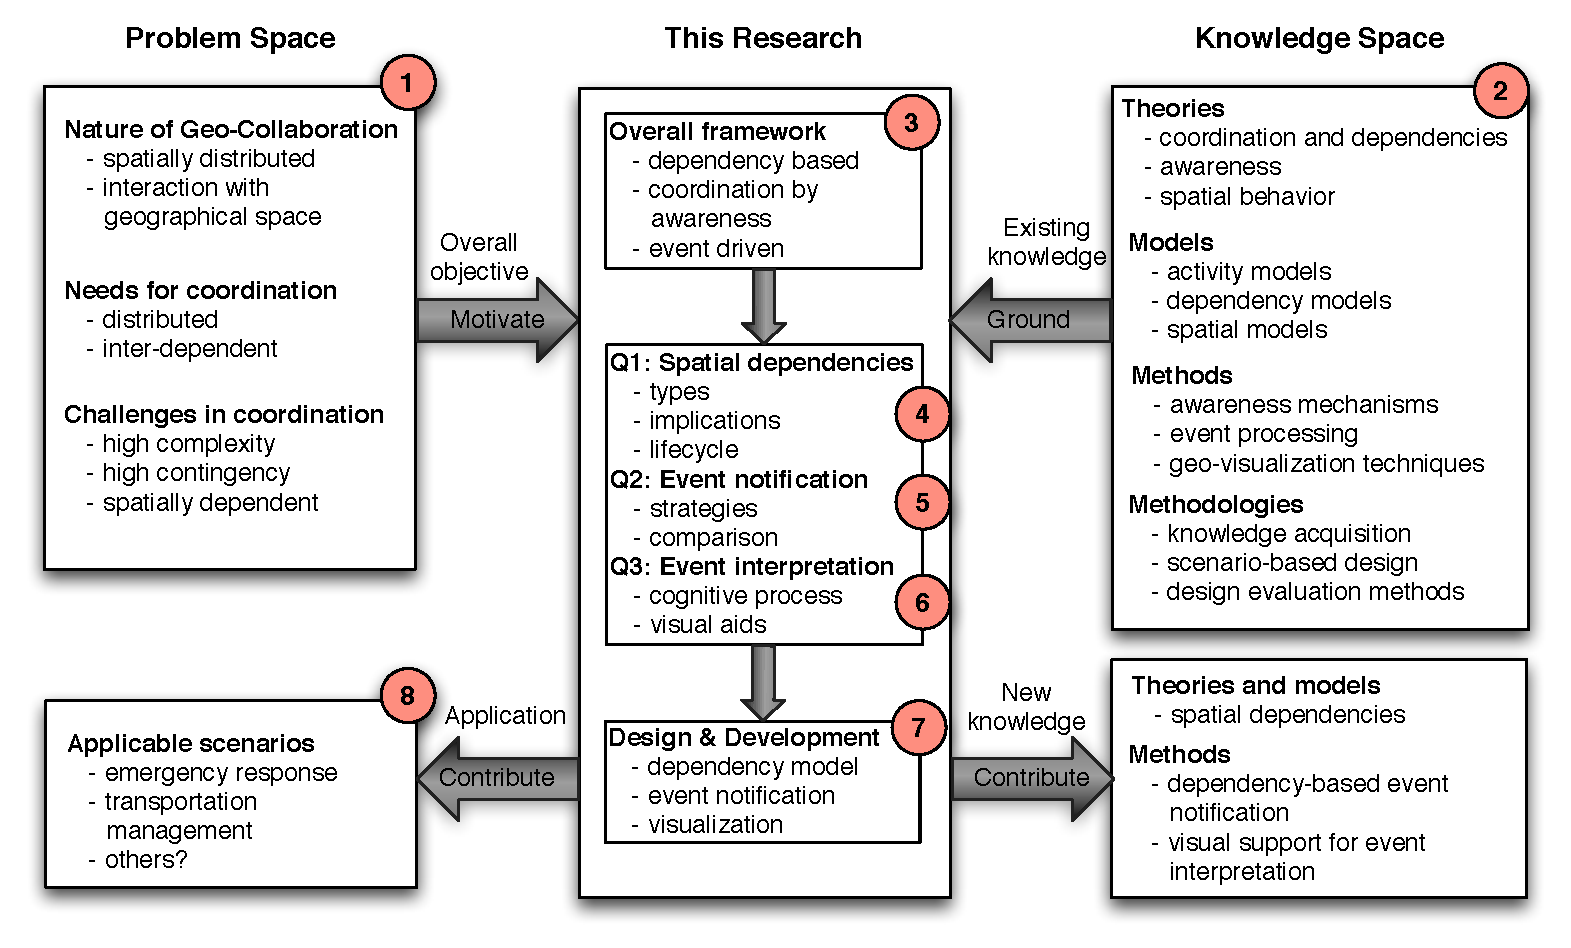
\includegraphics[width=5.8in]{research_overview.pdf} 
   \caption{Overview of the research approach}
   \label{fig:research_overview}
\end{figure}

The research starts with defining the problem scope and specifying the design challenges in the problem scope (Chapter \ref{chapter1:introduction}). Then the existing knowledge about theories and models to understand the awareness phenomena is reviewed to provide the theoretical foundation of this study (Chapter \ref{cha:understanding_awareness}). Based on the grounding work in the literature, we develop the conceptual framework to understand the awareness phenomena in large-scale distributed collaboration (Chapter \ref{cha:the_conceptual_framework}). Such a conceptual framework help us to develop concrete design issues that need to be addressed, identify knowledge gaps in existing studies, and guide our design of the awareness promotion approach (Chapter \ref{cha:awareness_promotion}, \ref{cha:knowledge_reprsentation_and_updating}, and \ref{cha:promoting_event_driven_awareness}). Following the computational approach, we develop the prototype system to prove the feasibility of the approach (Chapter \ref{cha:system_implementation}). Then we perform the case study in a concrete emergency response scenario to demonstrate the utility of our approach in support awareness in large-scale distributed collaboration (Chapter \ref{cha:case_studies}). 

Following the design-research paradigm, the contributions of this research include (1) the development of conceptual models that extend and improve the understanding of the design problem, (2) and the development of methods or tools that enable solutions to the design problem (Chapter \ref{cha:conclusion}).

\begin{enumerate}
	\item The first major contribution of this research is the integrated conceptual model for understand the awareness phenomena in large-scale distributed collaborations. Our conceptual model is built on top of existing theories and models, and in turn contribute to existing knowledge foundations in two aspects: (1) Beyond the knowledge sharing perspective, we emphasize the distributed nature of the awareness phenomena. Because of the differences in local scopes, each team member’s awareness is partial, but at the same time is compatible for the team to perform collaborative activities successfully. (2) Comparing with existing models, our framework provides a better explanation of how the compatibility of different collaborators’ awareness is achieved through the integration of individual cognitive processes and social processes.
	\item The second major contribution of this study is the awareness promotion approach that aims to design a knowledge-based awareness system that maintains a collective knowledge representation of the collaborative work, and utilizes it to support the various awareness processes. With the help of the formal knowledge representation, the awareness promotion approach shows several advantages to handle the scaled up complexity and dynamics in collaborative activities, and provides integrated awareness support.
\end{enumerate}
% section research_approach_and_contributions (end)
%!TEX root = ../BoYu-Dissertation.tex
\graphicspath{{Figures/}}
\chapter{Understanding Awareness} % (fold)
\label{cha:understanding_awareness}

\fxfatal{Add a general diagram to layout the framework, discuss existing work in the framework, add a table to compare and summarize the literature}

The concept of awareness has come to play a central role in both social and technical research in CSCW. However, what in CSCW labeled as `awareness' has little in common, besides the fact that it represents some aspect of human interaction that is important for successful collaboration \cite{schmidt2002a}. In a broad sense, two types of awareness can be distinguished in the CSCW research area: \emph{social awareness} and \emph{task-oriented awareness} \cite{prinz1999a,schmidt2002a}.

\emph{Social awareness} addresses the availability of different kinds of information about the social context of the team members, e.g. awareness about what they are doing, if they are talking to someone, if they can be disturbed etc. \emph{Social awareness} thus is conceived of as something that engenders ``informal serendipitous interactions'' \cite{hudson1996a} and ``a shared space for community building'' \cite{Dourish1992}. Awareness of the general social context is an important aspect of collaborative work, especially in domains where the the actors are engaged in cooperative work in a loose and broad sense, or domains where socialization is crucial \cite{schmidt2002a}.

However, when the tasks of collaborating actors become closely interdependent on each other, more urgent concerns need to be given to the aspect of \emph{task-oriented awareness}. The \emph{task-oriented awareness} focuses on practices through which actors seamlessly align and integrate their distributed and yet interdependent activities, e.g. awareness of things being done or in need of being done, of developments within the joint effort that may be advantageous or detrimental for one’s own work, of occurrence that makes one’s work more urgent or leads to changes to the intended course of actions, etc. \cite{schmidt2002a}. The major difference of \emph{task-oriented awareness} from \emph{social awareness} is that it focuses on activities performed to achieve a specific shared goal \cite{carroll2003a} and the actor’s being interdependent in their work \cite{schmidt2002a}, which lead to the unavoidable requirement for coordination.

In this study, we focuses on the \textbf{task-oriented aspect of awareness}, because the primary goal of supporting awareness in this study is motivated by the actors' being interdependent in their work and hence by the unavoidable requirements of coordinating and integrating their various actions in distributed geo-collaborative activities.

Within the scientific investigation into task-oriented awareness phenomena in collaboration, two lines of research can be identified. On one hand is the research aiming to establish conceptual understanding of the awareness phenomena from the cognitive and social aspects \cite{Salmon2008}, and on the other hand is an increasing bearing on system design and development in particular technologies to promote awareness \cite{rittenbruch2009a}. Although our work has an emphasis on the second aspect, i.e. the supportive technologies to promote awareness, we believe that a solid conceptualization of awareness phenomena in collaboration is extremely important for awareness promotion. System designers need to know what awareness might comprise and also how it is built and maintained in order to identify the specific awareness features they want to support \cite{Stanton2006}. 

As a result, before we move to the computational issues for awareness promotion, this chapter attempts to identify which of the existing theories and conceptualization of awareness in the literature is the most suitable for understanding the awareness phenomena in real world complex collaborative activities. A review and critique of what is currently known on the concept of awareness at both individual and team levels is presented, following which an integrated conceptual framework of awareness phenomena in complex collaborative activities is presented. In next chapter, we will show how such a conceptual framework helps us to evaluate existing computational awareness models and systems, and informs our design of the computational framework for awareness promotion.

\section{Situation Awareness}
\label{sec:awareness_in_individuals}
Research into awareness at the individual level originated from the study of situation awareness (SA) in the human factors research community. Situation awareness is considered as knowledge created through interaction between a person and his/her environment, i.e. ``knowing what is going on'' in the situation \cite{Endsley1995}. A good general definition of situation awareness is as ``the up-to-the minute cognizance required to operate or maintain a system'' \cite{Adams1995}. Although most of the situation awareness models in the literature are individual focused theories \cite{Salmon2008}, it has also been well recognized as an important element in collaborative environments. For example, Gutwin and Greeenberg \cite{Gutwin2002} view their workspace awareness as a specialization of situation awareness tied to the specific setting of the shared workspace. The concept of activity awareness proposed by Carroll et al. also subsumes situation awareness with an emphasis on aspects of the situation that have consequences for group work towards shared goals \cite{carroll2003a}. Hence, to understand the awareness phenomena in collaboration, it is important to start with understanding the practice of how individuals maintain and develop the situation awareness.

The human factors community has not settled on a common explanation of situation awareness, but we still can summarize some of the important characteristics that are well recognized in the literature, and also applicable to collaborative environments:

\begin{enumerate}
	\item The products of awareness is the knowledge about the elements of the environment that is hierarchically structured \cite{Endsley1995}.
	\item The awareness phenomena should be seen as both product and process. As product, it is the knowledge that an actor can make use of. As process, it includes the cognitive processes through which the knowledge is achieved and developed) \cite{Adams1995}.
	\item The process of achieving and developing awareness revolves around internally held, mental models, which contain activated information regarding current situations \cite{Smith1995}. The activation of awareness information into the mental models are directed by the actor's activity \cite{Bedny1999}.
\end{enumerate}

We elaborate these three characteristics in the following of this section.

\subsection{Hierarchically Structured Awareness Knowledge} % (fold)
\label{sub:awareness_as_product}
Among the numerous attempts at specifying the products of situation awareness, i.e. what must be known to solve a class of problems posed when interacting with a dynamic environment \cite{Salmon2008}, Endsley's three-level model \cite{Endsley1995} has undoubtedly received the most attention. The three-level model describes situation awareness as the operator's internal model of the state of the environment, comprising three hierarchical levels that is separate to the process used to achieve it \cite{Smith1995}:

\begin{enumerate}
	\item Level 1: \emph{perception of relevant elements in the environment}. An actor must first be able gather perceptual information in the surrounding environment, and be able to selectively attend to those elements that are most relevant for the task at hand. At this stage, the information is merely perceived and no further processing takes place. 
	\item Level 2: \emph{Comprehension of task-related elements in Level 1}. Level 2 involves the interpretation of the perceptual information from Level 1 in a way that allows an actor to comprehend or understand its relevance in relation to their tasks and goals.
	\item Level 3: \emph{Projection of the states in the near future}. Using a combination of Level 1 and Level 2 awareness-related knowledge and experience in the form of mental models, actors forecast likely future states in the situation.
\end{enumerate}

Endsley's three-level model presents an intuitive description of situation awareness and has been applied in a plethora of different domains \cite{Wickens2008}. Its simplicity and the division of SA into three hierarchical levels allows the construct to be measured easily and effectively \cite{endsley1995measurement}, and also supports the abstraction of situation awareness requirements and the development of design guidelines \cite{Salmon2008}. Furthermore, it has been extended in order to describe team situation awareness \cite{endsley2001model}, and the three levels of awareness information are applicable in many collaborative situations \cite{Gutwin2002}.

Despite its popularity, the three-level mode has some important flaws. One of the key assumptions of the three-level model is the separation between depicting situation awareness as a product and the cognitive processes used to achieve it \cite{Salmon2008}, which leads to the inability to cope with the dynamic nature of situation awareness \cite{Smith1995}. For example, Uhlarik and Comerford \cite{uhlarik2002review} suggest that the process of achieving situation awareness presented by the three-level model is both static and finite. Nevertheless, the model is also criticized by the ill-defined concept of mental models. Although Endsley's model emphasizes the critical roles of mental models in directing attention to critical elements in the environment (Level 1), integrating the elements to aid understanding of their meanings (Level 2), and generating possible future states (Level 3), the definition only includes the long-term knowledge that is formed by training and experiences, more important factors, such as the actor's goals, conceptual model of the current situation, are neglected \cite{Bedny1999}.
% subsection awareness_as_product (end)

\subsection{The Development of Awareness} % (fold)
\label{sub:awareness_as_process}
To address the dynamic nature of situation awareness, many researchers have used Niesser's perceptual cycle model \cite{neisser1976cognition} to clarify the cognitive components involved in the acquisition and development of situation awareness \cite{Smith1995,Adams1995,Gutwin2002,Stanton2009}. According to the perceptual cycle model (Figure. \ref{fig:perceptual_cycle}), an actor's interaction with the world continues in an infinite cyclical nature. By perceiving the available information in the environment, the actor modifies its knowledge. Knowledge directs the agent's activity in the environment. That activity samples and perhaps anticipates or alters the environment, which in turn informs the agent. The informed, directed sampling and/or anticipation capture the essence of behavior characteristic of situation awareness.

\begin{figure}[htbp] %  figure placement: here, top, bottom, or page
   \centering
   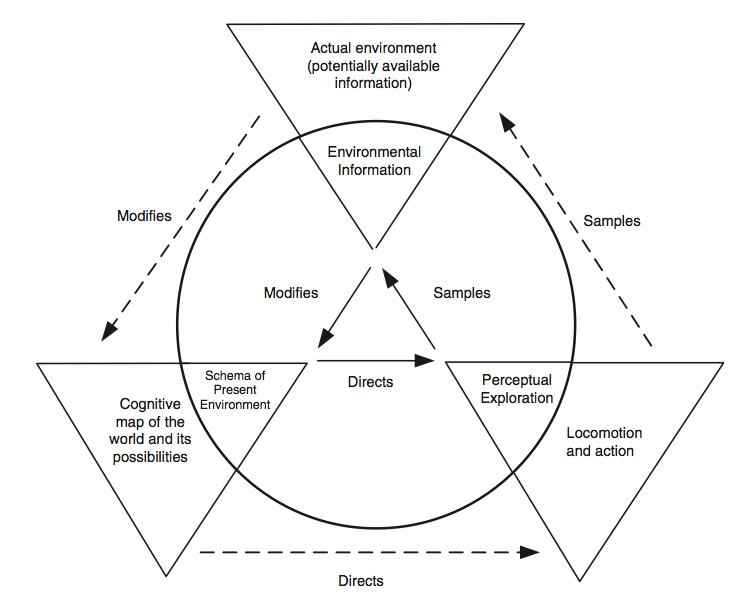
\includegraphics[width=5in]{perceptual_cycle.jpg} 
   \caption{Niesser's Perceptual Cycle Model \cite{Salmon2008}}
   \label{fig:perceptual_cycle}
\end{figure}

Based upon Niesser’s perceptual cycle model, Smith and Hancock suggest that situation awareness is neither resident in the world nor in the person, but resides through the interaction of the person with the world \cite{Smith1995}. Thus they viewing situation awareness as a generative process in `an adaptive cycle of knowledge, action and information' \cite{Smith1995}. In a similar fashion, Adams et al. \cite{Adams1995} used a modified version of Niesser’s perceptual cycle model to describe how situation awareness works. They argue that the process of achieving and maintaining situation awareness revolves around internally held mental models, which facilitate the anticipation of situational events, directing an actor's attention to cues in the environment and directing their eventual course of action. An actor then conducts checks to confirm that the evolving situation conforms to their expectations. Any unexpected events serve to prompt further search and explanation, which in turn modifies the actor's existing model. Gutwin and Greeenberg used the perception-action cycle to explain how the awareness is maintained in a shared workspace, in which awareness knowledge both directs and is updated by perceptual exploration of the workspace environment \cite{Gutwin2002}.

Unlike the three-level model that depicts SA as a product separate from the processes used to achieve it, models based on the perceptual cycle view situation awareness as both process and product, offering an explanation of the cognitive activity involved in the development of situation awareness, and also a judgment as to what the product of SA comprises \cite{Salmon2008}. One of the key assumptions of these models is the interplay between the awareness information and the internal mental model of current situation. In the process of awareness development, some knowledge is activated and integrated into the mental model, while some becomes inactive or removed from the mental model. Although Smith and Hancock suggested that the adaptation of awareness information into the mental model should be goal-directed, i.e. it must reside in the task environment rather than in the actor's head \cite{Smith1995}, little detail has been given about the cognitive processes that guide the selection and interpretation of awareness information into the mental models.
% subsection awareness_as_process (end)

\subsection{Activity Directed Awareness Process} % (fold)
\label{sub:activity_directed_awareness_process}
Bedny and Meister propose a description of situation awareness based on the activity theory in an attempt to clarify the cognitive processes involved in the interpretation of awareness information \cite{Bedny1999}. Based on the activity theory, they purport that individuals possess goals that represent an ideal image or desired end state of activity, which direct them towards the end state or methods of activity (or actions) that permit the achievement of these goals. It is the difference between the goals and the current situation that motivates an individual to engage in the awareness process and take action towards achieving the goal. They conceptualize activity in three stages: the orientational stage, the executive stage, and the evaluative stage. The orientational stage involves the development of an internal representation or picture of the world or current situation. The executive stage involves proceeding towards a desired goal via decision-making and action execution. Finally, the evaluative stage involves assessing the situation via information feedback, which in turn influences the executive and orientational components.

Instead of considering the actor's internal mental model as a whole, they suggest that the mental model is comprised of several functional blocks as presented in Figure \ref{fig:activity_sa}. Each functional block has a specific role to play in the development and maintenance of situation awareness and that the blocks orientate themselves towards the achievement of situation awareness. The interpretation of incoming information (function block 1) is influenced by an individual’s goals (function block 2), conceptual model of the current situation (function block 8), and past experience (function block 7). This interpretation then modifies an individual’s goals and experience and conceptual model of the current situation. Critical environmental features are then identified (function block 3) based upon their significance to the task goals and the individual’s motivation towards the task goal (function block 4), which directs their interaction with the world (function block 5). The extent to which the individual proceeds to engage the task goals is determined by their goals (function block 2) and their evaluation of the current situation (function block 6). The resultant experience derived from the individual’s interaction with the world is stored as experience (function block 7), which in turn informs their conceptual model (function block 8).

\begin{figure}[htbp] %  figure placement: here, top, bottom, or page
   \centering
   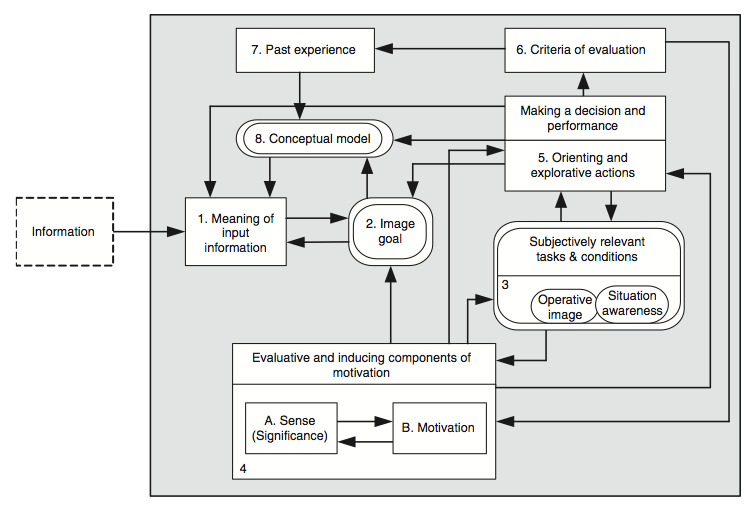
\includegraphics[width=5.5in]{activity_sa.jpg} 
   \caption{Bedny and Meister's Activity-Directed Awareness Process \cite{Bedny1999}}
   \label{fig:activity_sa}
\end{figure}

Based on the activity theory, Bedny and Meister clearly elucidate the functional blocks within the actor's mental model and their roles in the development of situation awareness \cite{Bedny1999}. Their model clearly shows how the actor's goals and activities play a central role to drive the process of awareness development. However, like most other situation awareness-related models, Bedny and Meister's activity theory model does not attempt to cater for, or explain the awareness phenomena in collaborative settings.
% subsection activity_directed_awareness_process (end)

\section{Awareness In Collaboration} % (fold)
\label{sec:awareness_in_collaboration}
The awareness phenomena in collaborative environments is indubitably more complex than situation awareness at the individual level. Salas et al. \cite{salas1995situation} point out that there is a lot more to team level awareness than merely combining individual team member's situation awareness. Beyond knowing what is going on in the environment, in their tasks, team members also need to develop an understanding of the activities of others, which provides a context of their own activities. This context is used to ensure that individual contributions are relevant to the group's shared goal as a whole \cite{dourish1992awareness}. This section reviews three prominent conceptualizations of awareness in collaboration that informs this study: team situation awareness, activity awareness, and distributed team awareness.

\subsection{Team Situation Awareness} % (fold)
\label{sub:team_situation_awareness}
The research on team situation awareness (TSA) attempts to extend the theories and models of situation awareness to collaborative settings. Endsley et al. \cite{endsley2001model} suggest that, during team activities, situation awareness can overlap between team members, in that individuals need to perceive, comprehend and project awareness elements that are specifically related to their specific role in the team, but also elements that are required by themselves and by members of the team. Successful team performance therefore requires that individual team members have good situation awareness on their specific elements and also the same awareness for those elements that are shared. It is therefore argued that, at a simple level, team situation awareness comprises three separate but related components: individual team member's situation awareness; situation awareness of other team members; and situation awareness of the overall team (Figure \ref{fig:tsa}). 

\begin{figure}[htbp] %  figure placement: here, top, bottom, or page
   \centering
   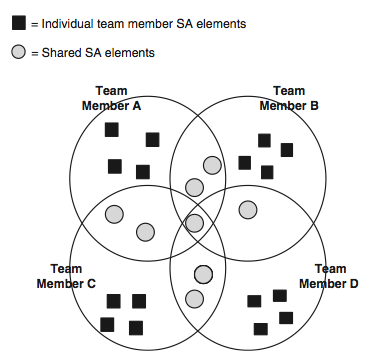
\includegraphics[width=3.5in]{TSA.jpg} 
   \caption{Team Situation Awareness (adapted from Endsley 1995 \cite{Endsley1995})}
   \label{fig:tsa}
\end{figure}

Similar to individual situation awareness, team situation awareness should be considered as a dynamic process. Salas et al. \cite{salas1995situation} propose a framework of team situation awareness that comprises two critical processes, individual situation awareness and team processes. According to them, team situation awareness depends on communications at various levels. The perception of SA elements is influenced by the communication of mission objectives, individual tasks and roles, team capability and other team performance factors. The comprehension of awareness information (i.e. Level 2) is impacted by the interpretations made by other team members, so it is evident that SA leads to SA and also modifies SA, in that individual SA is developed and then shared with other team members, which then develops and modifies team member SA. Thus, a cyclical nature of developing individual SA, sharing SA with other team members and then modifying SA based on other team members’ SA is apparent. 

Most attempts to understand team SA have centered on a `shared understanding' of the same situation. Nofi \cite{nofi2000defining}, for example, defines team SA as: `a shared awareness of a particular situation' and Perla et al. \cite{perla2000gaming} suggest that `when used in the sense of ``shared awareness of a situation'', shared SA implies that we all understand a given situation in the same way'. Shu and Furuta sugggested that TSA comprises both individual SA and mutual awareness and can be defined as `two or more individuals share the common environment, up-to-moment understanding of situation of the environment, and another person's interaction with the cooperative task' \cite{shu2005inference}.

Team situation awareness has been broadly recognized as a critical factor to understand awareness in collaborative environment, because its compatibility to individual situation awareness, and the abstraction of individual awareness process from team processes \cite{shu2005inference,Salmon2008}. However, TSA also has many limitations.

\begin{enumerate}
 	\item First, a critical factor of team situation awareness is to define the configuration of shared situation awareness requirements, i.e. the degree to which team members understand which information is needed by which team member, or by the whole team. The identification of such shared awareness requirements is feasible in simple, small-scale collaborative scenarios However, for complex, real world collaborative scenarios, such a task becomes more intricate. In complex scenarios that involve numerous agents and artifacts working both collaboratively and dispersed geographically, viewing and assessing team situation awareness is actually too complex \cite{Salmon2008}. 
 	\item Second, the role of team processes, such as communication, mutual monitoring, in maintenance and development of team situation awareness, is only barely touched. It is recognized that an increased level of team processes will lead to enhanced levels of team situation awareness. However, the specific relationships between team situation awareness and team processes remains largely unexplained \cite{Salmon2008}.
 	\item Last, the team situation awareness adopts the knowledge-in-common view of shared mental models \cite{Mohammed2001}, i.e. it focuses on how the shared understanding of the same situation is developed. However, as argued by Mohammed and Dumville, the knowledge-in-common view may be appropriate for only certain task domains and types of groups \cite{Mohammed2001}. For example, in teams with high level of division of work, the distribution of knowledge and skills across the team typically is not uniform, as a result, a high level of overlapping knowledge in such teams might be inefficient.
 \end{enumerate} 

% subsection team_situation_awareness (end)

\subsection{Activity Awareness} % (fold)
\label{sub:activity_awareness}
To address the problem of team situation awareness that posits `knowledge in common' as a basis for awareness, Carroll et al. proposes a new framework for understanding awareness in collaborative environment, based on the concept of `activity awareness' \cite{carroll2003a,carroll2006a}. The major distinction between team situation awareness and activity awareness is that, in realistically complex circumstances, instead of merely sharing relatively static and stable constructs such as knowledge in common, people share their activities \cite{carroll2006a}. In framing activity awareness, they appropriate the concept of \emph{activity} from Activity Theory to emphasize that collaborators need to be aware of a whole, shared activity as complex, socially embedded endeavor, organized in dynamic hierarchies, and not merely aware of the synchronous and easily noticeable aspects of the activity \cite{Carroll2009}. 

Similar to the activity-directed SA model proposed by Bedny and Meister \cite{Bedny1999}, activity awareness emphasizes the importance of using the concept of activity to structure the products and processes of awareness phenomena. The ultimate motivation of human actors to acquire and maintain awareness in the collaborative environment is to achieve their shared goals by performing their activities. As a result, the context surrounding a collaborative activity (e.g. the manner in which a shared activity is decomposed into smaller inter-related tasks, how these subtasks are assigned or adopted by collaborators, and when and how distributed subtasks are interdependent on each other), becomes the most important aspects of the situation that the team members need to be aware of \cite{carroll2003a}.

By shifting the focus from shared knowledge to shared activity, activity awareness aligns the development of awareness with the development of collaborative activities. Most basically, activity awareness is achieved and developed through the join construction of common ground - shared knowledge and beliefs, mutually identified and agreed upon by members through a rich variety of communication protocols \cite{carroll2006a}. In long-term, open-ended activities over significant spans of time, the construction of shared practices, social capital, and human development become also important to enhance team member's activity awareness.

Activity awareness with its basis on Activity Theory, primarily focuses on the social aspect of the awareness phenomena, i.e. how the team members' awareness of the social context of collaborative activities is developed through common grounding, construction of shared practices, social capital, and human development. Although the authors claim that activity awareness subsumes situation awareness \cite{carroll2003a}, little discussion has been given to how these higher-level social processes are connected to the cognitive processes to maintain situation awareness. Issues, such as how the state change in the external environment can lead to a team member's internal goal change, which could furthers lead to re-planning of their activities, cannot be explained. 

Furthermore, the activity awareness focuses on the sharing of activities, i.e. the importance of a common picture of the shared collaborative activities. However, such a common picture is usually distributed in the whole group, instead of in any single actor's mind \cite{Stanton2009}. Each actor in the group has their own awareness, related to the goals they are working towards. However, this seldom includes the whole picture of the collaborative activity, and only when all the actors' awareness knowledge is meshed up together, the common picture emerges. Activity awareness framework provides little support to explain how the activity knowledge is distributed across multiple actors.
% subsection activity_awareness (end)

\subsection{Distributed Team Awareness} % (fold)
\label{sub:distributed_team_awareness}
A more recent theme to conceptualize awareness in collaboration is the concept of distributed or systemic team awareness \cite{Stanton2009,artman1998situation}. Distributed team awareness approaches are borne out of distributed cognition theory \cite{hutchins1995cognition}, which describes the notion of joint cognitive systems comprising the people in the system and the artifacts that they use. Within such systems, cognition is achieved through coordination between the system units \cite{artman1998situation} and is therefore viewed as an emergent property (i.e. relationship between systemic elements) of the system rather than an individual endeavor. Distributed team awareness approaches therefore view awareness in collaboration not as a shared understanding of the situation, but rather as a characteristic of the socio-technical system itself \cite{artman1998situation}. Whilst recognizing that team members possess their individual SA for a particular situation and that they may share their understanding of the situation, distributed team awareness assume that awareness is distributed across the different human and technological agents involved in collaborative systems \cite{Stanton2009}.

The main difference between distributed team awareness and other TSA and activity awareness models relates to the concepts of \emph{compatible} and \emph{shared} awareness. \emph{Shared} awareness accounts suggest that efficient team performance is dependent upon team members having the same awareness knowledge. Distributed team awareness, on the other hand, postulates that, within collaborative systems, different team members have unique, but \emph{compatible} awareness, regardless of whether the information that they have access to is the same or different \cite{Stanton2009}. Team members experience a situation in different ways, as defined by their own personal experience, goals, roles, tasks, training, skills, and so on. So whilst some of the information required by two different team members may be `shared' in the sense that they both need to attend to it as part of their job, their resultant understanding and use of it is different \cite{Salmon2010}. Ultimately, the picture developed by each team member is unique for themselves. \emph{Compatible} awareness is therefore the phenomenon that holds distributed systems together. Each team member has their own awareness, related to the goals that they are working towards. Although different team members may have access to the same information, differences in goals, roles, the tasks being performed make them view it differently. In this way, each team member’s awareness is different in content, but is compatible in that it is all collectively required for the system to perform collaborative activities successfully.

While the distributed team awareness emphasizes the distribution of awareness, it does not discount the social interactions among different team members. The term `transactive' awareness is used to describe the notion that distributed team awareness is acquired and maintained through \emph{transactions} that arise from communications or other team processes \cite{Salmon2010}. A transaction in this case represents an exchange of awareness between one agent and another (where agent refers to humans and artifacts). Agents receive information, it is integrated with other information and acted on and then passed on to other agents. The interpretation on that information changes per team member. The exchange of information between team members leads to transactions in the SA being passed around. For example, an agent may perceive certain awareness element in the environment, interpret the meaning, and then pass it to another agent via a transaction. The second agent then builds its own interpretation upon the first agent's interpretation, and may start a new transaction to pass the awareness to other agents. Hence, it is the systemic transformation of awareness elements as they cross the system boundary from one team member to another that bestows upon awareness in collaboration an emergent behavior \cite{Stanton2009}.

The concept of distributed team awareness has been investigated by the authors in a number of domains, including naval warfare \cite{Stanton2006}, energy distribution \cite{Salmon2008a}, and air traffic control \cite{Stanton2009}. The major strength of the approach is related to the systemic approach that it advocates, which is more suitable to analyze the awareness phenomena in complex, real world collaborative activities \cite{Stanton2009}. However, the main weakness, as admitted by the authors, is also related to it complexity \cite{Salmon2010}. Similar to other team situation awareness models, it uses concepts as the basic unit to analyze awareness elements, which often leads to extremely large networks in order to represent all the concepts and their relationships. A possible remedy is to integrate the distributed team awareness with the activity-directed models and switch the focus from concepts to activities to understand the awareness phenomena.
% subsection distributed_team_awareness (end)

% section awareness_in_collaboration (end)

\section{An Integrated Conceptual Model of Awareness} % (fold)
\label{sec:discussion}
By reviewing the existing theories and conceptualizations of awareness, we believe that, instead of adopting one particular viewpoint, a suitable conceptual model for understanding the awareness phenomena in real world complex collaborative activities requires the integration of multiple constructs in the literature. Specifically, we identify the following requirements:

\begin{enumerate}
	\item \emph{The integration of individual cognitive processes and social processes.} As most theories and models of awareness in collaboration claim that individual situation awareness is still an important component in collaborative environment, the conceptual model should be able to account for both cognitive processes at the individual level and social processes at the team level, and emphasize on how these two aspects interplay with each other. 
	\item \emph{The integration of compatible and transactive aspects of awareness phenomena.} We agree with the distributed team awareness approaches \cite{Salmon2010} on that, because of the differences in goals, roles, the tasks being performed make, each team member’s awareness is different in content, but at the same time is compatible for the team to perform collaborative activities successfully. Hence, the conceptual model should be able to account for how the awareness is distributed across multiple team members, and meanwhile can interact with each other via transactions. 
	\item \emph{The integration of awareness and activity.} We resonate with the activity-directed SA model \cite{Bedny1999} and the activity awareness framework \cite{carroll2003a} to emphasizes the importance of using the concept of activity to structure the products and processes of awareness phenomena. As the purpose of human actors to acquire and maintain awareness in the collaborative environment is to achieve their shared goals by performing their activities, it is very natural to use the activities to structure their awareness requirements. 
\end{enumerate}

To satisfy these requirements, we propose an integrated conceptual model of awareness in complex collaborative activities, by combining multiple constructs in the literature. In general, the model has two major components: (1) an integrative model of activities, local scopes of work, and dependencies that form \textbf{the field of collaborative work}, (2) and \textbf{a set of awareness processes} built on top of it (Figure \ref{fig:conceptual_framework}). The goal of the former is to establish the necessary knowledge that is needed to understand the content of awareness, i.e. \emph{aware of what}, and the later focuses on the awareness processes, i.e. \emph{how awareness is achieved and developed}. In the following of this section, we elaborate each component in more details.

\begin{figure}[htbp] %  figure placement: here, top, bottom, or page
   \centering
   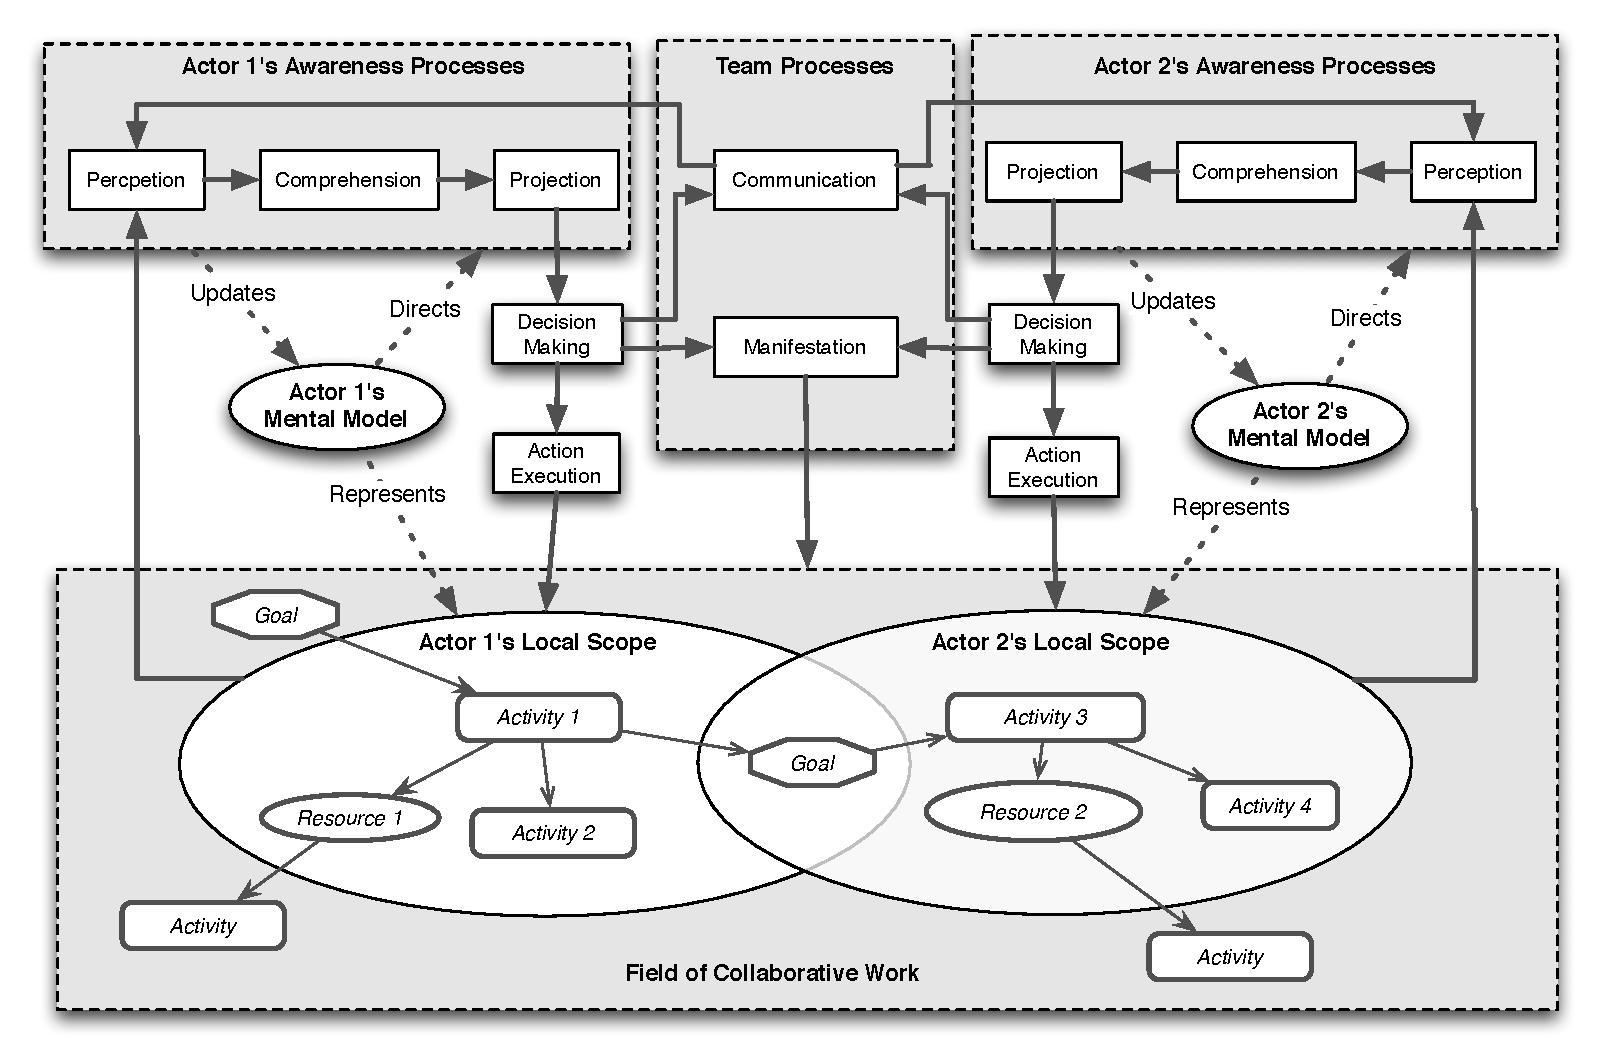
\includegraphics[width=5.5in]{conceptual_framework.pdf} 
   \caption{The Integrated Conceptual Model of Awareness}
   \label{fig:conceptual_framework}
\end{figure}

\subsection{The Field of Work} % (fold)
\label{sub:the_field_of_work}
Following the activity-directed SA model \cite{Bedny1999} and the activity awareness framework \cite{carroll2003a}, we focus on the concept of activity to structure the content of awareness, i.e. the field of collaboration work, built on top of three interrelated concepts:

\begin{enumerate}
	\item We consider \emph{activity} as the basic unit of analysis to support coordination in geo-collaboration.
	\item Due to the distributed nature of geo-collaboration, the various activities have different implications on different actors, and form their respective \emph{local scopes of work}.
	\item Activities in different local scopes of work are interdependent due to various types of \emph{dependencies} existing among them. Dependencies serve as the bridges between different local scopes of work to evaluate the implications of remote activities transcending multiple local scopes. 
	
\end{enumerate}

\subsubsection{Activity as the basic unit} % (fold)
\label{ssub:activity_basic_unit}
In our approach, we subscribe to Activity Theory to conceptualize human activities \cite{nardi1996context}. From this perspective, the basic structure of an activity can be defined as several basic elements and mutual relationships between them.

\begin{enumerate}
	\item \textbf{Actions} An action specifies a particular way of doing something. An action can be either basic or complex. A basic action can be directly executed by one or multiple actors. A complex action needs to be decomposed into subsidiary actions. When an action is specified as a sub-component of a higher action, this restricts the higher action to that particular course of doing. An action is assigned to a list of actors who are responsible to executing it.
    \item \textbf{Goals} A goal is a state of affairs in the world that the actors would like to achieve. How the condition is to be achieved is not specified, allowing alternatives to be considered. For example, a goal can only specify that a victim needs to be medically treated, but how it is achieved is not specified.
    \item \textbf{Actors} are defined as entities capable of performing actions and capable of making decisions on the performance of their actions. 
    \item \textbf{Resources} are anything that can be used in the transformation process of an action, including both material resource and resources for thinking. For example, in the case of response emergency, resources may include rescue vehicles, medical equipments, and information such as the locations of victims. 
\end{enumerate}
% paragraph relationships (end)
% subsubsection activity_basic_unit (end)

\subsubsection{Local scope of work} % (fold)
\label{ssub:local_scope_of_work}
Although various activities can be identified in a complex collaborative environment, each actor usually only engages in a small set of them. In fact, one of the fundamental motivations for team work is to decouple a complex problem into a set of smaller ones that are much easier to manage and tackle. One result of the decoupling is that the work of actors is distributed and each actor is only interested in the states of a small set of activities, resources, and conditions that are relevant to their roles, current goals and tasks. To characterize the distributed nature of team awareness, we define the local scope of work for each actor as the set of activities, resources, and conditions that have direct or potential impact on the actor’s work.

The concept of local scope of work have several characteristics of the distributed nature of emergency response activities:

\begin{enumerate}
	\item First, the local scope of work is a relative concept that changes with the actor’s current goals. Whenever an actor’s goal is changed, the local scope of work may also be changed.
	\item Second, the local scope of work may cover multiple portions of the collaborative activity as a single actor may focus on several activities at the same time. 
	\item Third, the local scopes of two actors can overlap with each other. It is common that the same activity, resource, or condition falls into the local scopes of different actors, even though it may have different impacts on these actors. Actually, these overlapping elements across multiple local scopes of work play an important role in supporting the transactive awareness process.
\end{enumerate}
% subsubsection local_scope_of_work (end)

\subsubsection{Dependencies} % (fold)
\label{ssub:dependencies}
Although activities are largely distributed and belong to local scopes of different actors, they cannot be performed without interacting with each other. Although an actor is only responsible for or interested in the activities within her/his local scope of work, the activities outside the local scope can still potentially impact her/his work through dependencies. 

Dependencies have been studied by many researchers with aspect to coordination, from organizational studies (\cite{yu1993actor,crowston1994taxonomy}), multi-agent systems (MAS) (\cite{sichman1998social,sikora1998a,sichman2002multi}), and computer-supported cooperative work (CSCW) (\cite{raposo2002coordination,cataldo2006a,de2007supporting}). Dependencies within a collaborative process can be of various forms. In general, we can summarize three types of dependency relationships that have been well recognized in the literature: temporal relationships, resource-related relationships, and goal-related relationships.

\begin{enumerate}
	\item \emph{Temporal dependencies.} The activities of the actors might be interdependent due to the constraint of ordering them in a certain order \cite{sikora1998a}. In some case, certain activities cannot be started until others are finished (the problem of sequencing) or a certain group of activities have to be performed at the same time (the problem of synchronization).
	\item \emph{Resource dependencies.} Resource dependencies can be analyzed in terms of common objects, i.e. resources, that are used by multiple actors or involved in multiple actions. An example is when two or more users simultaneously want to alter the same part of a document in a collaborative authoring system \cite{berlage1999a}. These common objects constrain how each activity is performed. Different patterns of use of the common objects by the activities will result in different kinds of dependency relationships \cite{malone1990coordination}: A \emph{fit dependency} occurs when multiple activities collectively produce the same resource. A \emph{flow dependency} arises whenever one activity produces a resource that is used by another activity. A \emph{sharing dependency} arises whenever multiple activities all use the same resource.
	\item \emph{Goal dependencies.} Goal dependencies involves the subsidiary goals that might be interdependent across various actors or their tasks \cite{sikora1998a}. A goal-related dependency reflects the fact that the depender depends on the dependee to bring about a certain state in the world. Unlike the temporal or resource-related dependencies in which the depender knows what tasks are involved in these relationships, the depender in a goal-related dependency does not care how the dependee goes about achieving the goal, i.e. the dependee is free to, and is expected to, make whatever decisions are necessary to achieve the goal \cite{yu1993actor}. A goal-related dependency is usually characterized by the structural relationship resulting from goal decomposition of the whole shared goal, i.e. task A depends on the other task B because B is a means to achieve a subsidiary goal that must be satisfied in order to perform A.
\end{enumerate}

\subsection{Awareness Processes} % (fold)
\label{sub:awareness_processes}
Built upon the field of work, a set of awareness processes can be identified to describe how the awareness is acquired and developed in a cyclical way (Figure \ref{fig:conceptual_framework}). In general, we can identify the awareness development cycles at both the individual and team levels.

\subsubsection{Individual Processes} % (fold)
\label{ssub:cognitive_processes}
At the individual level, each team member develops his/her own awareness in the similar way as described in the Neisser's perceptual cycle model \cite{neisser1976cognition}: the development of awareness starts with the perception of selective elements in the actor's local scope of work, which is then interpreted with the help of the actor's existing knowledge. The result of interpretation then help the actor to make certain decisions and perform actions, which then further update the actor's local scope of work. A important difference in our model from the original perceptual cycle model is that, instead of action directly stimulated by the acquired awareness knowledge, we emphasize the individual's planning process before the action performance, in which the individual needs to make decisions on what to do based on the interpretation of awareness information, such as whether he/she needs to change the goal, perform re-planning, or ask for help etc.

\begin{enumerate}
	\item \emph{Perception}. The process of perception is very similar to the concept in the perceptual cycle model. An actor must first be able gather perceptual information in the surrounding situation, and be able to selectively attend to those elements that are most relevant for the task at hand. The only difference is that the perception is constrained by the actor's local scope, i.e. he/she can only perceive the information about the environment, acitivities, or other objects defined in his/her local scope.
	\item \emph{Interpretation}. The process of interpretation includes generating the awareness knowledge at both the comprehension and projection levels in Endsley's three-level model \cite{Endsley1995}. The actor comprehends or understands the relevance of perceptual information in relation to their tasks and goals, and predicts likely future states in the situation.
	\item \emph{Planning}. The process of decision-making involves two major tasks. The first is to elaborate the actor's plan based on the interpretation. This involves decisions such as commitment to certain activity, focus switching, re-planning. The second task includes decisions about whether the actor wants to propagate the interpretation to other actors, which is important for initiating the awareness development cycle at the team level.
	\item \emph{Action}. Based on the result of decision-making process, the actor may perform some action to manipulate his/her local scope, which can lead to further changes that will start another round of perception.
\end{enumerate}

% subsubsection cognitive_processes (end)

\subsubsection{Team Processes} % (fold)
\label{ssub:interactive_processes}
Beyond the individual processes of awareness development, our conceptual model allows the transactive awareness development across multiple actors in a team. The development of awareness at team level can be performed explicitly or implicitly. Based on the interpretation of awareness information, an actor may decide to propagate the change to other actors by indicating how the other actor's activities can be impacted by his/her interpretation. The result of propagation is then perceivable by the other actor and may initiate the other actor's individual awareness development cycle. As the other actor develops his/her individual awareness, he/she may decide to propagate his/her interpretation back to the actor or other actors in the team, or he/she may perform actions that lead to changes in other actors' local scopes. In either way, new individual cycle may be initiated and the awareness development continues at the team level.

The development of awareness at the team level is guided by the dependencies among activities and the shared activities in overlapping local scopes. The dependencies allow the actors to cascade the awareness interpretation across multiple activities. The shared activities in overlapping local scopes enable the propagation process to cross the boundary of multiple local scopes.

\subsection{An Example} % (fold)
\label{sub:an_example}
We use the motivating emergency response scenario described in Chapter 1 to show an example of the conceptual framework. 

Figure \ref{fig:field_of_work} illustrates how the different activities are distributed into different local scopes of work (represented as dotted circles) and how they are connected by the various dependency relationships. As we can see from the example, the different actors in the scenario, the victim manager, the decontamination manager, and the transportation manager, have very different roles to play, and therefore their local scopes vary significantly. However, due to the dependencies among their activities (For example, the decontamination manager relies on the transportation manager to deliver the victim to the decontamination station; the victim manager relies on the decontamination manager to perform decontamination on the victim), their local scopes are overlapped with each other.

\begin{figure}[htbp] %  figure placement: here, top, bottom, or page
   \centering
   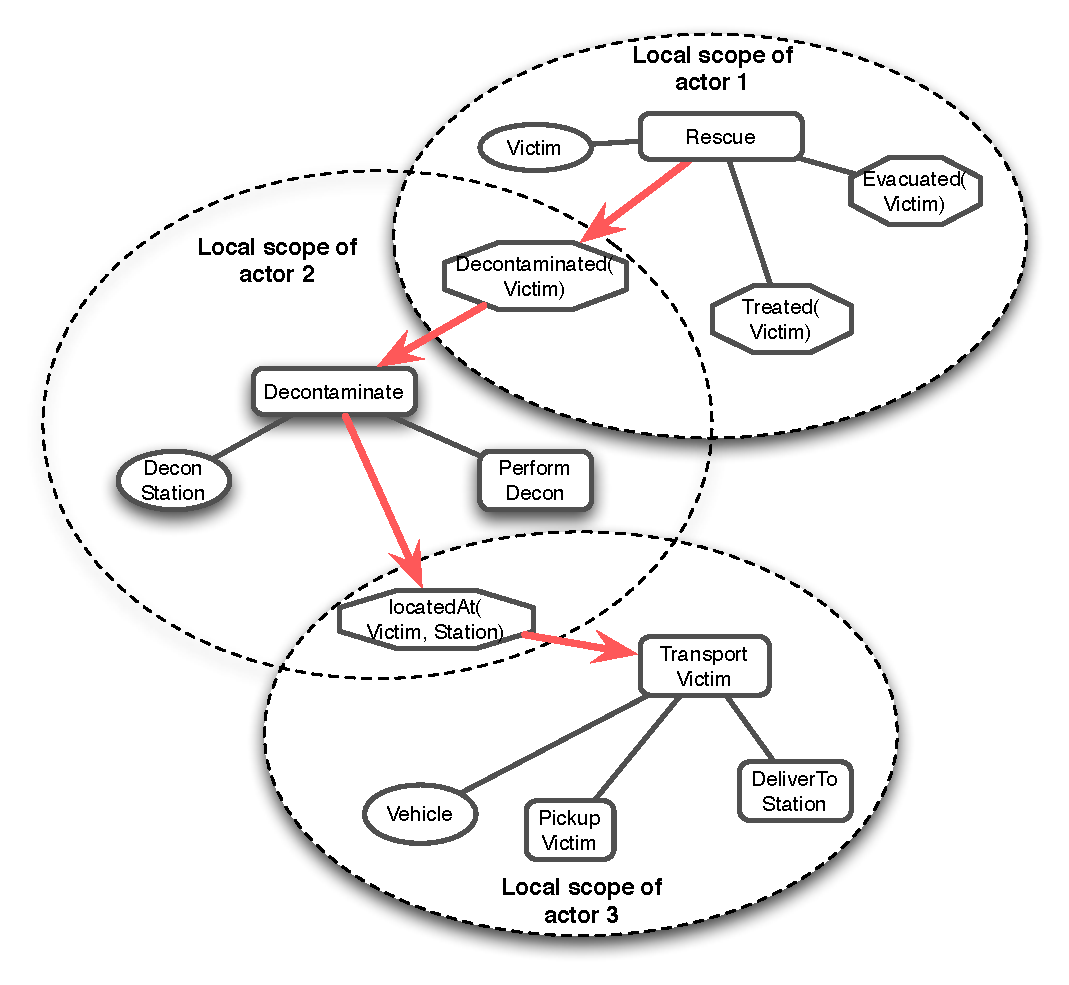
\includegraphics[width=4.5in]{field_of_work.pdf} 
   \caption{An Example: The Field of Work}
   \label{fig:field_of_work}
\end{figure}

Figure \ref{fig:awareness_process} demonstrates how the awareness processes work on top of the three constructs. In the beginning, Actor 1 perceives some unexpected event happening in the environment, and attempts to interpret it as whether and how it can impact the activities within her local scope of work. After understanding the event, she associates it with a state change of Activity 1. Furthermore, she predicts how the state change of this activity will impact other activities because of the dependencies among them. After Actor 1’s interpretation, the event is likely to impact another activity (Activity 2), and Actor 1 decides to propagate it. The propagated event falls into Actor 2’s local scope of work. Upon receiving this interpretation from Actor 1, Actor 2 first needs to understand where this event comes from by backtracking the interpretation, and evaluate how this event will impact his own line of work, which leads to a new projected state change of Activity 3. The similar process then is propagated to Actor 3’s local scope of work. In this way, the team’s awareness of the initial external event is collaborative developed as the relevant actors gradually attach their interpretations to it. 

\begin{figure}[htbp] %  figure placement: here, top, bottom, or page
   \centering
   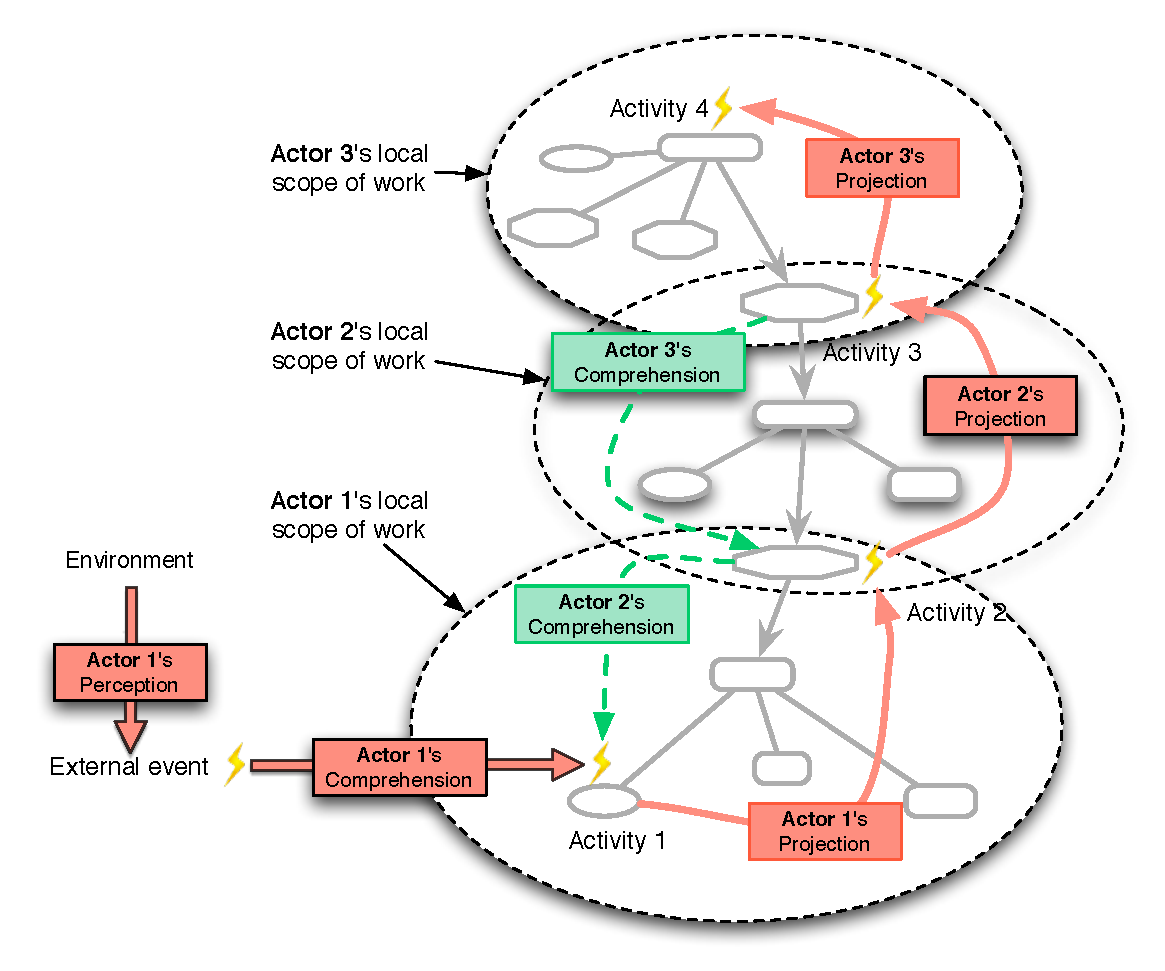
\includegraphics[width=4.5in]{awareness_process.pdf} 
   \caption{An Example: The Awareness Processes}
   \label{fig:awareness_process}
\end{figure}
% subsection an_example (end)
\subsection{Discussion} % (fold)
\label{sub:discussion}
The proposed conceptual framework shows the capabilities to satisfy the three requirements we presented in the beginning of this section.
\begin{enumerate}
	\item First, the conceptual model provides two ways to connect the individual cognitive processes and team processes. On one hand, the connection can be implicit as team members interact with the filed of work. The development of an actor's individual awareness can manipulate the field of work, which can then be perceived by other actors in their separate individual awareness processes. In addition, the actors can explicitly propagate their interpretations to other actors within their individual awareness processes.
	\item Second, the concept of local scope allows us to define how the awareness knowledge is distributed across multiple actors. The different actors often attend to different sets of activities as their local scopes. At the same time, the actors' local scopes are often overlapped due to the various dependency relationships that may occur between activities, this provides the mechanism to allow awareness transactions among multiple actors. In this way, the compatible and transactive aspects of awareness phenomena are integrated.
	\item Last, our structure of the field of work is based on the activity theory, which enables the integration of awareness and activity.  
\end{enumerate}
% subsection discussion (end)
% section discussion (end)

% chapter understanding_coordination (end)

%!TEX root = ../BoYu-Dissertation.tex
\graphicspath{{Figures/}}

\chapter{A Conceptual framework of Awareness in Large-Scale Distributed Collaboration} % (fold)
\label{cha:the_conceptual_framework}

% chapter the_conceptual_framework (end)




 


%!TEX root = ../BoYu-Dissertation.tex
\graphicspath{{Figures/}}

\chapter{Awareness Promotion} % (fold)
\label{cha:awareness_promotion}
The conceptual model of awareness presented in previous chapter clearly shows the complexity of the awareness phenomena in large-scale distributed collaborative activities:

\begin{enumerate}
   \item First, due to the highly distributed nature of the collaborative activities, team members play specialized roles and are engaged in different actions. As a result, each actor has distinct awareness requirement, related to the goals and actions that they are working towards.
   \item Second, in order to achieve the compatible awareness at the team level, each actor needs to be aware of more things than their individual awareness, and interact with each other.
   \item Last, because of the continuous development of the collaborative activities, the actors' awareness requirements are quite fleeting.
\end{enumerate}

Due to the increased complexity and dynamics, awareness can no longer be achieved effortlessly by the actors themselves, and computer support becomes an important component in awareness systems to augment and complement human capability. This chapter provides the overview of our computational approach to supporting awareness in large-scale distributed collaborative activities. The general design principle of our approach is to emphasize the active role of computer system to not merely support, but rather promote awareness in collaborative activities.

In this chapter, we first identify the major challenges for human actors to achieve and develop awareness in distributed, complex collaborative activities, which highlight the design aspects in which computer systems can provide support. Then we discuss how these design aspects have been addressed (or partially addressed) in existing awareness support systems. Last, we present our awareness promotion framework that has the potential to better address these challenges.

\section{Designing for awareness support} % (fold)
\label{sec:designing_for_awareness_support}
As described in Section \ref{sec:awareness_processes}, in order to achieve awareness, human actors have to engage in a variety of cognitive and social processes. In this section, we identify the major cognitive and interactive challenges for human actors in awareness processes at both the individual and team levels, and analyze how the system can provide support to augment and complement human capability correspondingly.

\subsection{Support for individual awareness} % (fold)
\label{sub:support_for_individual_awareness}
\paragraph*{Perception} % (fold)
\label{par:perception}
The achievement of individual awareness starts with the ability of individuals to perceive key awareness elements in the environment. As the complexity of the collaborative activities scales up, there are potentially a very large number of awareness elements that are available at any given time. However, due to the partiality of awareness, each actor is only interested in a small set of them that are relevant to his/her own task. As a result, human actors have to focus on filtering out a large number of irrelevant information, which may consume too much of the actor's attention resources. 

The computer can support the human actors in this process by reducing the number of awareness elements presented to the actors. If the system can predict the awareness needs of the actors, the effort of filtering out irrelevant information can be transferred to the computer systems, so that human actors can focus on processing only the relevant set of information to avoid information overload.
% paragraph perception (end)

\paragraph*{Comprehension} % (fold)
\label{par:comprehension}
Comprehension is to understand the meaning of perceived awareness information within the context of a user's current goals and activities \cite{oulasvirta2007a}. In the comprehension process, new awareness information must be combined with existing knowledge about the current collaborative activities, which provides the inferential framework \cite{carroll2003a} for the actor to evaluate which part of the collaborative activity will be impacted by the perceived awareness information. 

Without computer support, human actors have to maintain existing knowledge about the collaborative activities in their minds. However, in large-scale collaborative activities where the magnitude of the collaborative work can grow significantly as hundreds or thousands of actors engaged in myriads of interdependent activities, it becomes a challenging task for human actors to maintain such an inferential framework in the mind. Alternatively, there are two ways that the comprehension can be supported by computer systems: 

\begin{enumerate}
   \item First, the computer system can support human comprehension by providing external representations of the existing knowledge. Instead of merely relying on the internal representations of human users, the external representation can serve as the information store, so that the internal representation at a given time can be quite sparse, perhaps containing only detailed information about their current focus \cite{Hegarty2011}, or pointers to locations of other important information in the external representation \cite{M.1996}. In this way, the limited working memory resources of human users are freed up for other aspects of cognition \cite{M.1996}.
   \item Second, the computer system can directly aid the linking between new awareness information and existing knowledge by presenting the awareness information along with the contextual information that is potentially relevant to understand its meaning \cite{Tomaszewski2010}. Supporting comprehension by linking has its basis on the design principle of offloading cognitive processes onto perceptual processes \cite{M.1996}. By explicitly linking the awareness information to contextual information for interpretation, some complex cognitive processes, such as searching for and activating the relevant portion of existing knowledge, can be replaced by simple pattern recognition processes \cite{Hegarty2011}. 
\end{enumerate}
% paragraph comprehension (end)

\paragraph*{Projection} % (fold)
\label{par:projection}
Projection is the process that the individual predicts the future states of other activities based on the comprehension of awareness information. As argued by Endsley \cite{Endsley1995}, this is the most difficult and taxing part to achieve individual awareness because it requires a fairly well developed mental model of the activities and relationships among them, and the capabilities to perform reasoning. The analytical reasoning is central to the projection process, through which users identify possible alternative future scenarios and the signs that one or another of these scenarios is coming to pass \cite{Thomas2006}. Similar to the comprehension, when the complexity of collaborative activities scales up, it becomes a challenging cognitive task for human actors due to the large volume of knowledge that needs to be stored and managed during the reasoning process. The computer support for projection, as a result, can be supported from two aspects:

\begin{enumerate}
   \item Similar to the comprehension process, the projection process can be supported by providing external representations of the existing knowledge and the analytic tools to allow the users to synthesize information and derive insight from it.
   \item On the other hand, the system can perform the reasoning tasks and simply present the reasoning results to the actors. In this way, the high level reasoning tasks are transformed into low level perceptual tasks for the actors.
\end{enumerate}
% paragraph projection (end)
% subsection support_for_individual_awareness (end)
\subsection{Support for collaborative awareness} % (fold)
\label{sub:support_for_collaborative_awareness}
As we described in Section \ref{sub:development_of_collaborative_awareness}, the development of collaborative awareness is mediated by the transactions between multiple actors through which actors' individual awareness processes are connected as developmental trajectories. As a result, besides the individual awareness processes, the actors have to perform the team processes to conduct awareness transactions.

The challenges for actors to perform the team processes for awareness development can be analyzed from two aspects: the overhead of maintaining additional transactive knowledge and the extra effort to perform team processes. 

\paragraph*{Transactive knowledge} % (fold)
\label{par:transactive_knowledge}
In order to conduct awareness transactions, the actors need to attain more knowledge than what is needed for their individual work. In general, we can identify two types of knowledge that are necessary for the actors to conduct awareness transaction.
\begin{enumerate}
   \item First is related to the concept of `transactive memory' that describes how the individual memories of team members are supplemented by the additional knowledge about other actors \cite{wegner1987transactive}. Within the context of collaborative awareness, that means, in order to conduct awareness transactions, the actors need to maintain knowledge about how each other's work is related. To monitor each other's work, the actors need to know who else's work may have impact on their own work. To externalize or communicate their individual awareness to others, the actors need to know whose work may be impacted by my work or my interpretation on the awareness information.  
   \item The other is the knowledge about the historical development of the awareness. As we described in the conceptual model of awareness, the awareness information perceived by the actor may not be directly generated from the environment, rather it can be the result of multiple awareness transactions among several actors. In order to understand the meaning of the perceived awareness information, the actor may have to trace back to understand where it comes from, who else has been impacted or contributes to its development, etc.
\end{enumerate}

As the complexity of collaborative activities scales up, maintaining these two types of knowledge increases the actors' cognitive overhead significantly. With the increased number of actors and possible dependencies among their actions, the knowledge about other actors whose actions are related to an actor grows rapidly. In addition, there are more actors participated in each developmental trajectory, so that it becomes difficult for the actors to keep track of the historical development of the awareness.

Correspondingly, the computer system can support the actors by maintaining the two types of transactive knowledge for the human actors. Whenever the actors need the knowledge, they can turn to the computer system to retrieve it. Moreover, the computer system can make use of the knowledge on behalf of human actors and perform reasoning to facilitate the awareness transactions. If the computer system knows whose actions to monitor, the system can monitor them for the actors. If the computer knows who needs to be notified by a piece of awareness information, it can deliver it to the relevant actors without human intervention.
% paragraph transactive_knowledge (end)

\paragraph*{Team processes} % (fold)
\label{par:team_processes}
Besides the additional knowledge that is needed, the awareness transactions are often achieved by some sort of team processes, such as direct communication or externalization in which the actors externalize some intentional aspects of their individual awareness and make them visible to others. These team processes pose an additional effort for the actors who initiate the awareness transactions. However, the actors who perform these team processes, i.e. the \emph{initiators} of team transactions, are often not the actors who will directly benefit from them, i.e. the receivers of team transactions. The disparity between cost and benefit \cite{Grudin1994} becomes an important challenges for the awareness development, as it may discourage the actors to conduct the awareness transactions.  As a result, in order to support the development of collaborative awareness, the computer system needs to provide effective tools for the actors to perform the team processes, so that the extra effort can be minimized.
% paragraph team_processes (end)
% subsection support_for_collaborative_awareness (end)

Table \ref{tab:design_aspects} summarizes the major challenges for human actors and the supporting aspects for computer systems to support the awareness processes.
{\footnotesize
\begin{longtable}{>{\raggedright}p{1.2in}>{\raggedright}p{2.2in}>{\raggedright}p{2.2in}}
\toprule 
\textbf{Awareness Process} & \textbf{Challenges for human actors} & \textbf{Design aspects for computer support}\tabularnewline
\midrule 
\multirow{3}{1.2in}{Development of individual awareness} & \emph{Percpetion}: they have to filter out a large number of irrelevant
information, consuming their attention resources & \emph{1.} \emph{Filtering}: the computer predicts the awareness needs
and filters out irrelevant information for human actors.\tabularnewline
\cmidrule{2-3} 
 & \emph{Comprehension}: they have to maintain a large volume of knowledge
about the collaborative activities in their minds & \emph{1. Representation}: the computer provides external representations
of the existing knowledge to free up human working memory resources.

\emph{2. Linking}: the computer presents the awareness information
along with the contextual information that is potentially relevant
to understand its meaning.\tabularnewline
\cmidrule{2-3} 
 & \emph{Projection}: they have to maintain the large volume of existing
and derived knowledge during the reasoning process  & \emph{1. Representation}: the computer provides external representations
and analytic tools to allow the human actors to synthesize information
and derive insight.

\emph{2. Reasoning}: the computer performs the reasoning tasks and
presents the reasoning results to human actors.\tabularnewline
\midrule 
\multirow{3}{1.2in}{Development of collaborative awareness} & \emph{Transactive knowledge}: they need to maintain transactive knowledge
that increases their cognitive overhead significantly & \emph{1. Representation}: the computer provides external representations
of the transactive knowledge.

\emph{2. Reasoning}: the computer makes use of the knowledge on behalf
of human actors and performs reasoning to facilitate awareness transactions.\tabularnewline
\cmidrule{2-3} 
 & \emph{Team processes}: they need to spare additional effort to conduct
team processes, but are often not the actors who will directly benefit
from them. & \emph{1. Tools}: the computer needs to provide the tools that simplify
the effort to perform team processes.\tabularnewline
\bottomrule
\caption{Design aspects for awareness support}
\label{tab:design_aspects}
\end{longtable}   
}
% section designing_for_awareness_support (end)

\section{Existing studies} % (fold)
\label{sec:the_state_of_art}
By outlining the design aspects for awareness support in Section \ref{sec:designing_for_awareness_support}, we can use them to review existing studies on awareness systems by looking into how the design aspects have (or have not) been supported. Before that, we need to make a distinction between two types of computational models for organizing and processing awareness information: \emph{space-based} and \emph{event-based} models, because it is the underlying computational model that determines how the awareness processes are supported in an awareness system \cite{Gross2004}.

\subsection{Computational models of awareness support} % (fold)
\label{sub:awareness_models}
Most awareness systems rely on certain computational models for organizing and process awareness information. A computational model usually provides a representation of the field of work, and specifies how awareness information is generated on top of it. In general, we can distinguish two types of awareness models commonly used in existing awareness systems: \emph{space-based} and \emph{event-based} models. 

\subsubsection{Space-based models} % (fold)
\label{ssub:space_based_model}
Many researchers have previously described systems to support awareness based on the spatial metaphor \cite{Benford1993,Rodden1996,Sandor1997,simone2002a}. These space-based models explicitly represent the various shared objects, which might represent actors, information, resources, or other computer artifacts, situated and manipulable in some space. Awareness is then achieved by the interaction between actors within the space, as they present themselves and attend to each other in the space \cite{Rodden1996}. Awareness information thus is implicitly embedded as perceivable properties of objects in the space.  

The use of space-based model relies on presenting a `shared space' among collaborators at any given time to provide awareness information, both implicitly and explicitly \cite{dourish1992awareness}. By maintaining the state of the shared work setting, people can either keep an eye on what the rest of the group is doing while doing their individual work, or actively monitor the activities of others, to perceive awareness information \cite{simone2002a}. 
In existing awareness systems, the `shared space' can take different forms \cite{antunes2010a}. 
\begin{enumerate}
   \item `Shared physical space'. In the early work of supporting awareness, a significant effort was devoted to exploring the potential of media space technologies, i.e. an array of continually audio-video links between distributed actors, to provide a `shared physical space' between actors in different locations \cite{Dourish1992}. As with the awareness study, the media space investigations were concerned with informal or social aspect of awareness, and in most cases task-oriented awareness was not mentioned explicitly \cite{schmidt2002a}.
   \item `Shared virtual space'. Rodden \cite{Rodden1996} developed the notion of `virtual space' as a collection of computer-supported interactive spaces. Many collaborative systems offer various types of virtual spaces to support awareness, including abstract media space \cite{Pedersen1997}, virtual meeting rooms \cite{Berlage1999}, and collaborative virtual environment \cite{Benford2001}. Unlike traditional media spaces that aim to establish the `shared physical space', this line of work focuses on the use of abstract representations as awareness indicators. Besides providing a kind of `shielding' for privacy of the people in the shared space \cite{Pedersen1997}, a more interesting feature of using abstract representations is the capability to organize awareness information around task-oriented structures, such as office tables, meeting rooms \cite{Berlage1999}, so that more task-oriented aspects of awareness can be supported.
   \item `Shared workspace'. `Shared workspace' is a specialization of the notion of `shared space' that emphasizes the task-oriented awareness. According to Gutwin and Greenberg \cite{Gutwin2002}, a `shared workspace' is a bounded space where people can see and manipulate artifacts related to their activities. A group editor is a good example of this type of `shared workspace', as it serves to organize activities like writing and revising, while maintaining a coherent view of the whole \cite{dourish1992awareness}. The awareness information in `shared workspace' is presented by attaching it to the manipulable objects through which the task is carried out, and is achieved by user's interaction with the artifacts \cite{Gutwin2002}.
\end{enumerate}
% subsubsection space_based_model (end)

\subsubsection{Event-based models} % (fold)
\label{ssub:event_based_model}
\emph{Event-based} models, on the other hand, provide people with awareness of what is going on around them as expressed by discrete events \cite{rittenbruch2009a}. Each event highlights a piece of awareness information related to certain state change in a collaborative setting for a limited amount of time. Events can be generated by sensors that are associated with actors, shared material, or any other objects that constitute or influence a cooperative environment \cite{prinz1999a}. The list of events that are supported in each awareness system can be totally different, depending on the application domain. As argued by Fuchs et al \cite{Fuchs1995}, we can basically imagine any kind of event, as long as it has a certain relevance when it comes to coordinating the work in a given setting. 

Unlike space-based models where the awareness information is implicitly embedded as properties of objects in the underlying representation of shared spaces, awareness information is explicitly represented as first-class objects in event-based models. Each event contains identifiers of the originator, the time, the state change in the collaborative setting, and the context in which the state change took place \cite{fuchs1999a}. Modeling awareness information as first-class objects decouples it from the objects or artifacts in the collaborative activities, which provides several distinguishing features from the space-based models:

\begin{enumerate}
   \item It allows the awareness information refers to any aspects of the collaborative activities, not only the external aspects, but also the internal aspects reflecting the intentions and beliefs of the actors.
   \item The awareness information is not limited within the user's current viewpoint. The user may attend to their own individual work in the filed, but still be able to receive events about other users that are outside his/her current viewpoint. 
   \item The awareness information is pushed to the users when the event happens, so that the actors does not need to spare their attentional resource to monitor each other's work.
\end{enumerate}

Because of the decoupling of awareness information from the representation of collaborative work, many existing event-based systems actually do not need to provide an explicit shared representation of the collaborative work \cite{prinz1999a,Fitzpatrick2002}.  Even in some systems where the collaborative work is represented (for example, the GroupDesk \cite{Fuchs1995} and the POLIAwaC systems \cite{sohlenkamp2000po} use semantic networks comprised of actors, artifacts, events, and their relations; the BSBW system \cite{Bentley1995} and Atmosphere model \cite{Rittenbruch2002} use hierarchical structures of workspaces), they are mainly used by the designers to specify events and manage event distributions, and are invisible to the actors.
% subsubsection event_based_model (end)

Table \ref{tab:awareness_models} shows a summary of the major distinguishing features of the \emph{space-based} and \emph{event-based} models. In the following of this section, we will discuss details on how the design aspects in various cognitive and social processes as shown in Section \ref{sec:the_design_space} have (or have not) been supported each of these models.

{\footnotesize
\begin{longtable}{>{\raggedright}p{1.1in}>{\raggedright}p{2.2in}>{\raggedright}p{2.2in}}
\toprule 
 & \textbf{Space-based models} & \textbf{Event-based models}\tabularnewline
\midrule 
\multirow{2}{1.1in}{Representation of the collaborative work} & explicitly represented as a `shared space' inhabited by objects representing
actors, information, resources, or other computer artifacts  & implementation-dependent internal representations\tabularnewline
\cmidrule{2-3} 
 & visible to users & invisible to users\tabularnewline
\midrule 
\multirow{4}{1.1in}{Awareness information} & embedded as perceivable properties of objects in the space & explicitly represented as discrete events\tabularnewline
\cmidrule{2-3} 
 & limited to external aspects of shared objects  & can refer to both external and internal aspects\tabularnewline
\cmidrule{2-3} 
 & presented in the context of its origin & can be outside the user's current viewport\tabularnewline
\cmidrule{2-3} 
 & users need to pull the awareness information from the field of work & awareness informaion is pushed to the users\tabularnewline
\midrule 
Example Implementations & 1. physical spaces (e.g. Portholes \cite{Dourish1992})

2. virtual spaces (e.g. AROMA \cite{Pedersen1997},
DIVA \cite{Berlage1999}, MASSIVE-2 \cite{Benford2001})

3. workspaces (e.g. ShrEdit \cite{dourish1992awareness},
GroupKit \cite{Roseman1996}) & GroupDesk \cite{Fuchs1995}, POLIAwaC \cite{sohlenkamp2000po},
NESSIE \cite{prinz1999a}, Elvin \cite{Fitzpatrick2002}\tabularnewline
\bottomrule

\caption{The main distinguishing features of space-based and event-based models}
\label{tab:awareness_models}
\end{longtable}
}

One thing to note is that, in many existing awareness systems, the space-based and event-based models are not exclusive, rather they are combined together to provide an integrated awareness supporting environment. Many shared workspace systems, such as the GroupDesk \cite{Fuchs1995}, the POLIAwaC \cite{sohlenkamp2000po}, and the ENI \cite{Gross2004} systems, present a shared workspace among the collaborators, and at the same time supports event notifications. Atmosphere model \cite{Rittenbruch2002} uses hierarchical structures of workspaces, i.e. spheres, to represent the shared collaborative work, and they are also used to specify events and manage event distributions.
% subsection awareness_models (end)

\subsection{Awareness support in existing systems} % (fold)
\label{sub:awareness_support_in_existing_systems}

\subsubsection{Support for perception} % (fold)
\label{ssub:support_for_perception}
The support for perception regards filtering awareness information for human actors, which has been described in both \emph{space-based} and \emph{event-based} systems.

\paragraph*{Space-based systems} % (fold)
\label{par:space_based_systems}
Systems adopting the space-based awareness model usually depend on the various relationships between objects inhabiting in the shared space to decide on the relevance of awareness information.

Benford et al.'s spatial model \cite{Benford1993} provides a formal approach to managing awareness levels between objects inhabiting in a common spatial frame. Awareness between objects is manipulated via \emph{focus} and \emph{nimbus}, two subspaces within which an object chooses to direct either its presence or its attention. Then the awareness information is selected based on the overlapping between the receiver's \emph{focus} and the performer's \emph{nimbus} in certain medium \cite{Benford1993}. Anything about the performer happens in the overlapping area will be perceivable to the receiver. 

The original spatial model has been extended in several ways to support different awareness systems. Sandor et al. \cite{Sandor1997} redefined the concepts of \emph{focus} and \emph{nimbus} upon a semantic network that forms a representation of the working context, and use them to build a generic model `Aether' for supporting awareness in collaborative systems. Rodden \cite{Rodden1996} adopted an object-oriented approach to generalize the spatial model to provide notions of presence, sharing and awareness applicable to applications lacking a spatial metaphor. Simon and Bandini \cite{simone2002a} based on the spatial mode to propose the reaction-diffusion model that can support more user adaptation and dynamic features. Instead of using \emph{focus} and \emph{nimbus}, the awareness information is distributed using field and sensitivity function that allow for a more flexible and compact way of representing various types of nimbi and foci. 

Although various space-based models differ from each other in the specific calculation of awareness levels, the most important point emphasized in all of this work is the insistence that the selection of awareness information is a joint-product between the performer and the receiver, i.e. how the receiver directs the attention to the performer (\emph{focus}) and how the performer projects the presence or activity to the receiver (\emph{nimbus}).
% paragraph space_based_systems (end)

\paragraph*{Event-based systems} % (fold)
\label{par:event_based_systems}
Filtering awareness information in event-based systems focuses on managing events subscriptions that are used by human actors to describe their awareness interests. Many mechanisms that enable the event subscriptions have been discussed in the literature, and they vary from each other depending on how the filters are defined. 

\begin{enumerate}
   \item In the GroupDesk system \cite{Fuchs1995}, Fuchs et al. define several filters that allowed the limit of the flow of events. On the actor’s side there was an individual privacy filter that allowed the actor to set privacy policies for the events gathered about him. On the perceiver’s side an individual interest filter allowed the perceiver to subscribe only to the events in which he or she was interested. A global filter would allow for the filtering of general conditions (e.g., to comply with organizational policies). Definition of filters in the system is based on individual event types, which consist of a mapping from a set of event types to a list of interested users. The drawback of event type-based filtering is that it requires the user to explicit his/her interest on each event type in a predetermined way, which is a tedious task that the users are not always willing to perform \cite{Grudin1994}. Furthermore, the type-based subscriptions tend to be too rigid or unable to adapt to the team development \cite{Alarcon2002}.
   \item Alternatively, Elvin \cite{Fitzpatrick2002} adopts the content-based filtering of events. It describes events using a set of named attributes of simple data types and consumers subscribe to sets of events using boolean subscription expressions. When a notification is received at the Elvin server from a producer, it is compared to the consumers’ registered subscription expressions and forwarded to those whose expressions it satisfies. A key benefit of content-based notification is the capability to reduce the effort needed to manage event subscription. Instead of subscribing to each type of events, users can subscribe to event patterns, which can describe a set of events. In addition, content-based subscriptions allow the definition of composite events.
   \item ENI \cite{Gross2004} extends the content-based filtering approach and integrates the notion of `contexts' into the model. Context information includes locations, artifacts and applications and other information, which is linked to a specific context. ENI adds this information to existing event information in an awareness system. The model is based on two concepts of context. First, the model tries to determine the context of origin for each event. The authors suggest a context mapping mechanism that maps events gathered from sensor information against rules saved in a context database. Second, the model identifies the work context of the user who is receiving the notification. The work context is derived from the selection of shared workspaces. Based on the two types of context, then the filtering is performed on context matching, i.e. the user defines what types of event context he/she wants to receive in a specific work context. The context-based model tries to improve the event filtering by gathering additional information and allowing users to receive awareness information in a more context-specific manner. However, the context mapping mechanisms underlying this concept is highly complex, and it lacks a formal model to specify the two types of context.
\end{enumerate}
% paragraph event_based_systems (end)

\paragraph*{Comparison} % (fold)
\label{par:comparison}
The space-based systems rely on the users to monitor the shared spaces and perceive the relevant awareness information. As the whole field of work as a shared space is explicitly visible to each user, they can pick up the awareness information relevant to them even when their own interests have been changed. This provides more flexibility to handle increased level of dynamics. However, space-based systems become much more problematic when the level of complexity in collaborative activities increases. When the numbers of objects, actors and their actions are significantly increased, representing them in a shared space and relying on the users to monitor and filter awareness information from it becomes a challenging task, as it requires a lot of extra attentions and efforts from the users.

Event-based models provides a more lightweight way to present awareness information, as only the aspects of awareness information that is of relevance are presented. Furthermore, the event-based presentation is pushed to the users by making the events more perceivable to the users. In this way, the users do not need to switch their attentions to other’s activities until the event notification happens. As a result, event-based models can handle more complex situations than space-based models. However, the effectiveness of event-based models largely depends on the quality of event subscriptions, which often requires that considerable domain knowledge be explicitly embedded. As argued by Fuchs et al. \cite{fuchs1999a}, event-based systems seem to work satisfactorily for situations where workflow can be clearly defined in advance or if the application is known from the beginning. When the level of dynamics increases in collaborative activities, such condition can no loner hold. The user's awareness needs are often in the flux of changes, as their activities evolve. Hence, the event-based models becomes less effective in high level of dynamics.
% paragraph comparison (end)
% subsubsection support_for_perception (end)

\subsubsection{Support for comprehension} % (fold)
\label{ssub:support_for_comprehension}
The computer support in the comprehension process comes from two aspects: the computer provides external representations of the existing knowledge to free up human working memory resources, and links the awareness information along with the contextual information that is potentially relevant to understand its meaning. This is relatively an easier job in space-based systems and event-based models.

\paragraph*{Space-based systems} % (fold)
\label{par:space_based_systems}
In space-based systems, the explicit representation of the shared spaces provide the Most existing space-based systems provide visual-spatial displays \cite{Hegarty2011} of the shared spaces, which has a number of advantages to support comprehension. First, they organize information by indexing it spatially. In these displays, space in the display represents space in the field of work, so that if the representation of two items is close in the display, it is likely that those items are also close in the represented field of work. Therefore, information that needs to be related in interpreting and making inferences is likely to be represented by visual features that are close in the display \cite{Hegarty2011}. Second, they provide overviews of the whole field of work, and therefore can be perceived as a whole and provides necessary background for comprehending awareness information \cite{Berlage1999}. Furthermore, as the awareness information can be directly presented in the place of its origin, the user can offload the cognitive effort to locate the related objects onto perceptual processes \cite{M.1996}.

However, space-based systems also have limitations in supporting comprehension. First, we need to distinguish the difference between the context of \emph{origin} of the awareness information and the context of \emph{work} of the user who need to comprehend the information \cite{Gross2004}. Most space-based systems present the awareness information in place of the object where the information occurs on, i.e. within the context of its origin. However, what is more important in the comprehension process is for the user to understand the effects of the awareness information on his/her own work, i.e. within the context of the user's work. Second, the visual-spatial display of the whole field of work can become a difficult or even impractical task when the complexity of the collaboration scales up. When the number of actors, artifacts, and activities increases significantly, such a representation of the whole shared space will also become less efficient to support the comprehension. 
% paragraph space_based_systems (end)

\paragraph*{Event-based sytems} % (fold)
\label{par:event_based_sytems}
Event-based systems often do not provide explicit representation of the field of work. As a result, in order for the user to comprehend an event, he/she has to build and maintain a mental model of the inferential framework derived from the field of work, which increases the cognitive load for the user. To alleviate this problem, some event-based systems attempt to collocate event notifications within the context of work. For example, NESSIE provides the awareness information by the presentation of pictorial activity indicators for the members of a group as part of the shared workspace user interface \cite{prinz1999a}. In the virtual school project, Carroll et al. suggest that the deadlines and external events should be collocated with process and planning representations \cite{carroll2003a}. However, studies on supporting comprehension of events are still very limited. Questions such as what types of events should be collocated with what types of contextual representations are largely undetermined.
% paragraph event_based_sytems (end)

\paragraph*{Comparison} % (fold)
\label{par:comparison}
Support for comprehension can be achieved relatively effortlessly in space-based systems because of two features: the existence of an explicit representation of the shared space, and the possibility of presenting awareness information directly in the shared space. Comparing with space-based systems, the comprehension of events provides a more challenging task for the users, as the awareness information is typically presented in separate event-triggered displays peripheral to a person's current task-oriented concern \cite{carroll2003a}. 
% paragraph comparison (end)
% subsubsection support_for_comprehension (end)

\subsubsection{Support for projection} % (fold)
\label{ssub:support_for_projection}
To our knowledge, explicit support for projection is rarely discussed in existing awareness systems. The question about how new awareness information will lead to future changes in human actors' actions is usually considered as a cognitive task that is performed by human users. Since most of the space-based systems provide the external representation of the collaborative work, to some extent it can supports the projection by providing such external information store. However, the information represented in these shared spaces is often structured around the objects in the space. Many types of knowledge that is useful to predict future changes, such as the dependency relationships between actions, are not represented.
% subsubsection support_for_projection (end)

\subsubsection{Support for transactive knowledge} % (fold)
\label{ssub:support_for_transactive_knowledge}
Transactive knowledge in space-based systems can be supported by providing lightweight awareness widgets \cite{Gutwin1996}, along with the shared spaces. For example, DIVA uses a virtual office table to display participants in a chat room, as well as visualize their contributions over time\cite{Berlage1999}. The Babble system \cite{Erickson1999} includes a `social proxy' showing team member's level of contribution to a threaded discussion. These awareness widgets represent some aspects of the collaborators, so that the users can check them to figure out who they should interact with, or whether the actors are available for interruption. However, these lightweight awareness widgets mostly only display specific aspects of social awareness, such as the collaborator's arrival, availability, involvement, but cannot adequately support task-oriented awareness aspects \cite{carroll2003a}, such as the predicated status of their actions, the reasons behind their actions, or dependency relations between actions.

In event-based systems, transactive knowledge is usually represented as events that are related to the actors and their actions. For example, in AERE system \cite{fuchs1999a}, the status of other actors' actions are represented as activity events, so that the actors can maintain knowledge about the other participants through the events. However, the actors have to store the information carried in these events in their mind, which is less efficient than the space-based systems. The benefit of event-based system, on the other hand, is the capable to store history information about the awareness development. In many event-based systems, such as GroupDesk \cite{Fuchs1995} and NESSIE \cite{prinz1999a}, an event history is available so that the users can analyze the event history storage to understand how the events are developed. However, most systems store the events in the database as individual records, and do not provide the links between the events. In order to understand how the events are socially developed through transactions, they have to link them together based on their interpretations. 
% subsubsection support_for_transactive_knowledge (end)

\subsubsection{Support for team processes} % (fold)
\label{ssub:support_for_team_processes}
As we described in Section \ref{ssub:awareness_transactions}, the awareness transactions are supported by three types of team processes: mutual monitoring, direct communication, and externalization.

\paragraph*{Mutual monitoring} % (fold)
\label{par:mutual_monitoring}
In space-based systems, the process of mutual monitoring, i.e. making consequences of individual activities apparent to other participants, can be achieved either through the direct video-audio links between actors \cite{Dourish1992}, or through the artifact mediation \cite{Tee2009}. 

In media space-based systems, monitoring can be supported by the networks of audio and video to provide rich representation of people and their immediate surroundings \cite{Dourish1992}. By seeing others through the media space, it is believed that people can get a sense of others’ actions so that they can infer the consequences of their actions. However, Fish et al.’s study in the use of the Cruiser media space \cite{Fish1992} has shown that even though the media space allows the users to perceive each other's actions, it usually does not provide the visibility of the work artifacts involved in these activities. As a result, showing each other's activities does not necessarily mean the consequences of their activities can be fed through. 

As a result, a more common approach to mutual monitoring in space-based systems is through the common artifacts in the shared spaces, especially in shared virtual spaces and workspace \cite{Berlage1999}. In these systems, users' actions are organized around the common artifacts in the shared spaces, which supports the mutual monitoring through feedthrough \cite{dix1997challenges}, i.e., when artifacts are manipulated in some actions, they give off information that informs others the consequences of these actions \cite{Tee2009}. However, artifact-mediated feedthrough is limited to the aspects of users' actions that can be represented as some artifacts, the internal aspects of their actions cannot be supported.

In existing event-based systems, the process of mutual monitoring can be supported by a specific type of events, i.e. action events \cite{Fuchs1995}. Action events are generated by the system. Each time the state of an object changes due to some action of a user, a new event is generated to describe the change. Then the event is sent to the event processing server, and is distributed to the users who subscribe to it. Similar to the space-based systems, the aspects of actions are limited to the external aspects that can be observed by the computer systems.
% paragraph mutual_monitoring (end)

\paragraph*{Communication} % (fold)
\label{par:communication}
Communication is the prevalent form of team processes in awareness transactions, in which people explicitly talk about awareness elements with their collaborators \cite{Gutwin2002}. Computer mediated communication has been an important component in almost every distributed collaborative system, by providing team members a \emph{medium} to communicate with each other remotely. However, it is usually supported separately from the awareness systems as a standalone feature in collaborative applications.
% paragraph communication (end)

\paragraph*{Externalization} % (fold)
\label{par:externalization}
The basic way to support externalization in space-based systems is annotations, which are defined as hypertext nodes that are linked to the objects in the shared spaces \cite{Zheng2006,Weng2004}. Annotations allow the users to add their comments or interpretations on specific objects or locations in the shared space that are visible to other collaborators. In this way, annotations provide a way for the users to externalize their individual awareness and display them to others. However, annotations in space-based systems are often bound to the objects in the shared space, and therefore have limited capability to externalize other aspects of individual awareness, such as the intentions to perform actions, or state changes of actions. 

Rittenbruch et al. introduce and explore the notion of ``intentionally enriched awareness'' \cite{Rittenbruch2007}, which refers to the process of actively engaging users in the awareness process by enabling them to express intentions. ``intentionally enriched awareness'' emphasizes the role of actors to make some of their internal states (intentions, reasons, etc.) along with their actions visible to others. Their AnyBiff prototypical system is one of the limited existing attempts to support \emph{externalization} in awareness systems, which allows users to generate, share, and use a multitude of activity indicators to reveal intentions. The AnyBiff system is mainly used for supporting social awareness in relatively loose-coupled collaborative activities, and hence the information that the users can make visible to each other is very limited. In complex collaborative environments that we are interested in this study, we believe much more aspects of individual awareness could be made visible by the users. Supporting externalization involves not only help users express their intentions, but also make their interpretations of awareness information during comprehension/projection, or the results of their decision-making visible.
% paragraph externalization (end)
% subsubsection support_for_team_processes (end)
% subsection awareness_support_in_existing_systems (end)

\subsection{Summary} % (fold)
\label{sub:summary}
Table \ref{tab:awareness_models} shows a comparison of how the major design aspects of supporting awareness processes have been achieved in the \emph{space-based} and \emph{event-based} models.

{\footnotesize
\begin{longtable}{>{\raggedright}p{1.1in}>{\raggedright}p{2.2in}>{\raggedright}p{2.2in}}
\toprule 
\textbf{Awareness Processes} & \textbf{Space-based models} & \textbf{Event-based models}\tabularnewline
\midrule 
Percepetion & Make the shared space explicitly visible to each user, and rely on
human actors to pick up the relevant awareness information  & Filter information based events subscriptions that are generated by
human actors to describe their awareness interests\tabularnewline
\midrule 
Comprehension & 1. visualization of shared spaces

2. direct linking of awaress information to the context of its origin & Collocation event notifications into the display and control of work
objects \cite{prinz1999a,carroll2003a}.\tabularnewline
\midrule 
Projection & Visualization of shared spaces & rarely supported\tabularnewline
\midrule 
Mutual monitoring & 1. video-audio links \cite{Dourish1992}

2. artifacts mediated feedthrough \cite{Tee2009} & System generated events about actions \cite{Fuchs1995}\tabularnewline
\midrule 
Communication & separately supported & separately supported\tabularnewline
\midrule 
Externalization & annotations \cite{Zheng2006,Weng2004} & intention-enriched awareness events \cite{Rittenbruch2007}\tabularnewline
\bottomrule
\caption{Existing Studies in Awareness Support}
\label{tab:existing_studies}

\end{longtable}
}

Existing systems follow these two types of awareness models show some limitations to support the awareness phenomena as we conceptualized in Section \ref{cha:the_conceptual_framework}. 

\paragraph*{Supporting distributed awareness} % (fold)
\label{par:supporting_distributed_awareness}
Space-based models rely on the users to monitor the shared spaces and perceive the awareness information. This can be done efficiently if the local scopes of different users are largely overlapped, as the users can pick up the awareness information peripherally as they work on their own work \cite{schmidt2002a}. However, this becomes much more problematic when the actions of users are distributed and each of them is working on a different set of actions, as actively monitoring the shared space requires extra attentions and efforts from the users. On the other hand, event-based models provides more control on the users to decide on what aspects of awareness information that should be presented, so that the users do not need to switch their attentions to other’s actions until the event notification happens. However, awareness information in the form of events is usually presented separately from the inferential framework to comprehend it, which leads to extra effort in the comprehension process.
% paragraph supporting_distributed_awareness (end)

\paragraph*{Supporting dynamics of awareness} % (fold)
\label{par:supporting_dynamics_of_awareness}
Space-based models manage the awareness through the interaction of collaborators and rely on the users to monitor the field of work and perceive the awareness information. This provides more flexibility to handle increased level of dynamics. As the whole field of work as a shared space is explicitly visible to each user, they can pick up the awareness information relevant to them even when their own interests have been changed. On other other hand, event-based models largely depends on the quality of event subscriptions which usually need to be clearly defined in advance. When the level of dynamics increases in collaborative activities, the user's awareness needs are often in the flux of changes, as their activities evolve. Hence, the event-based models becomes less effective in high level of dynamics.
% paragraph supporting_dynamics_of_awareness (end)

\paragraph*{Supporting for higher-level individual awareness processes} % (fold)
\label{par:supporting_for_higher_level_individual_awareness_processes}
At the individual level, existing awareness systems have focused on supporting perception, the higher level of awareness processes are relatively less supported. A possible reason is that the higher-level awareness processes usually involve sophisticated cognitive and reasoning capabilities where the human can do better than the computer. As a result, most awareness systems leave the comprehension and projection to the users. However, in complex collaborative activities, as we discussed earlier, the scaling problem becomes significant, and hence it becomes much more important for the computer to provide functions to amplify and enhance human cognition, not only in the stage of perception, but also in comprehension and projection.
% paragraph supporting_for_higher_level_individual_awareness_processes (end)

\paragraph*{Supporting for awareness transactions} % (fold)
\label{par:supporting_for_awareness_transactions}
At the team level, existing awareness systems have focused on either supporting the explicit communication among human collaborators, or different approaches to providing `shared spaces' representing the fields of work so that the actions of each other become visible to each other. However, less discussion has been given to the explicit representation of transactive knowledge, or the externalization process, which actually is an even more important aspect of awareness in many complex, real world collaborative activities \cite{heath2002a}.
% paragraph supporting_for_awareness_transactions (end)
% subsection summary (end)
% section the_state_of_art (end)

\section{The awareness promotion approach} % (fold)
\label{sec:awareness_promotion_approach}
Our approach to supporting awareness in large scale distributed collaborative activities aims to address the design aspects described in Section \ref{sec:designing_for_awareness_support}, which only receive limited support in existing studies (Section \ref{sec:the_state_of_art}). In order to address these design aspects, we argue that the computer system needs to play a more active role to promote awareness among collaborators. In this section, we first present the rationale for awareness promotion, and then overview the computational awareness promotion framework.

\subsection{From awareness support to awareness promotion} % (fold)
\label{sub:from_awareness_support_to_awareness_promotion}
In existing awareness systems, the role of computer can be described in the metaphor of `tool' that emphasizes the human achieves his/her goal through the computer application \cite{Bodker1997}. In term of supporting awareness, it means the human actors use the computer to achieve awareness. The tool perspective emphasizes the control on the human user's side, i.e. how the computer is used to achieve awareness depends on the human user's own knowledge. For example, in space-based systems, the system relies on the user to monitor the shared space to perceive awareness information; in event-based systems, the user needs to explicitly express his/her interests so that the computer can filter out events. 

However, when the collaborative activities become more and more distributed and complicated, more is demanded of the human actors to control the computer. As we conceptualize the awareness phenomena as a distributed cognitive system (Chapter \ref{cha:the_conceptual_framework}), each human actor usually only has partial knowledge about the whole collaborative situation, and it is unlikely that the actor knows what exactly should be done in order to achieve awareness at the team level. With only local knowledge, the actor may have no idea what background information should be attended to in order to interpret a piece of awareness information that is out of his/her local scope of work. Or he/she cannot decide on who should be notified when his/her actions are changed. As a result, the user either uses the local knowledge to develop awareness that is often incomplete, vague, or even incorrect; or has to maintain more transactive knowledge beyond his/her local scope of work, which inevitably increases the user's cognitive load. 

As a result, we believe that merely relying on the user to control the computer to achieve awareness in distributed, complex collaboration is ineffective. Alternatively, a better approach is to allow the computer to take some control away from the user and actively perform some tasks to help the user to achieve awareness. Instead of relying on the user's internal, partial knowledge to control the awareness development, the computer can maintain a much more complete knowledge representation of the whole field of work at the systematic level, and make use of this knowledge to infer the user's awareness requirements in various awareness processes so as to provide adaptive support. In this way, the computer can be considered as a `mediator' actively engaged in the collaborative activities along with human actors, but with its own goal (i.e. to assist human actors to achieve awareness), its own mental model (i.e. the knowledge representation of the whole collaborative activity), and its own behaviors (i.e. the capabilities to reason about the user's need in the various awareness processes and adapt interaction and information presentation techniques to support it).

In general, we use the term `awareness promotion' to define the paradigm of awareness support where the computer plays an active role to mediate the awareness processes. While human actors still need to undergo the cognitive processes to develop individual awareness, and use it to make decision and perform actions in their own local scopes; the computer system takes the responsibility to maintain a collective picture of the whole collaborative activity, and utilizes this knowledge to facilitate the various cognitive and social awareness processes among human actors.

Table \ref{tab:awareness_support_vs_promotion} illustrates the major distinctions between the existing awareness support methods and the awareness promotion approach. From the table, we can clearly see the opportunities and benefits for active promotion in every awareness promotion processes.

\paragraph*{Promoting individual awareness} % (fold)
\label{par:promoting_individual_awareness}
The promotion of individual awareness can happen in all the three individual awareness processes. 
\begin{enumerate}
   \item In the perception process, instead of relying on human actors to decide on what information is relevant to them, the system can predict the human actors' needs and present the relevant information to the actors. Comparing with space-based systems, this promotion strategy has the capability to filter out the information for the actors to reduce the cognitive load. Comparing with event-based systems, this promotion strategy has two important benefits: (1) in these collaborative situations, the awareness information that is relevant to an actor may come from remote collaborators through multiple awareness transactions. The relevance of such awareness information is usually difficult for the actor to judge and describe in advance; (2) because of the dynamics of the collaborative activity, the interests of an actor in the awareness information may change frequently as the actor works on different actions. Predicting the actor's awareness needs as the activity proceeds reduces complexity to modify subscriptions.
   \item In the comprehension process, instead of presenting a whole shared space to the actors, the system can tailor the representation to only include the aspects of the collaborative activity that is relevant to the human actor, so as to improve the human actor's interpretation even when the whole collaborative activity becomes complex. In addition, the system can promote the comprehension by inferring how the awareness information is related to the human actors' actions in the local scopes, so that the human actors do not need to perform the inference by themselves.
   \item To promote the projection process, the system can also tailor the representation to only include the aspects of the collaborative activity that is relevant to the human actor's projection task. Furthermore, as the system represents the knowledge about the collaborative activity, the system can perform some of the routine inferences and present the results to the human actors, so as to convert some higher level cognitive tasks into some perceptual tasks for the actors.
\end{enumerate}
% paragraph promoting_individual_awareness (end)

\paragraph*{Promoting awareness transactions} % (fold)
\label{par:promoting_awareness_transactions}
The promotion of awareness transactions focuses on maintaining the transactive knowledge and the capability of the system to use the knowledge to distribute awareness information in the transactions. 
\begin{enumerate}
   \item The computer system can maintain the transactive knowledge at the team level, instead of for each actor to store the transactive knowledge in the mind. Whenever the actors need the knowledge, they can turn to the computer system to retrieve it. This becomes extremely important when the complexity of collaborative activities scales up, maintaining the transactive knowledge increases the actors’ cognitive overhead significantly.
   \item Moreover, the computer system can make use of the knowledge on behalf of human actors and perform reasoning to promote the awareness transactions. If the computer system knows whose actions to monitor, the system can monitor them for the actors. If the computer knows who needs to be notified by a piece of awareness information, it can deliver it to the relevant actors without human intervention. In this way, the human actors can only focus on externalize the aspects of their individual awareness, and leave the effort of monitoring and disseminating information to the computer system.
\end{enumerate}
% paragraph promoting_awareness_transactions (end)

{\footnotesize
   \begin{longtable}{>{\raggedright}p{1.1in}>{\raggedright}p{2.2in}>{\raggedright}p{2.2in}}
\toprule 
\textbf{Awareness processes} & \textbf{Awareness support} & \textbf{Awareness promotion}\tabularnewline
\midrule 
Percepetion & 1. the \emph{computer} shares information in a common space, and relies
on the \emph{human} to monitor the shared space to perceive information
(\emph{space-based} models)

2. the \emph{human} subscribes to events based on interests, and the
\emph{computer} filters out events based on human subscription\emph{
(event-based} models)  & the \emph{computer} infer who the information is relevant to, and
present only the relevant information\tabularnewline
\midrule 
Comprehension & 1. the \emph{computer} provides the representation of the whole shared
space

2. the \emph{computer} links the awareness information to the context
of its origin, and the \emph{human} infers the connection between
the context of origin and his/her work context & 1. the \emph{computer} only represents the aspects of the collaborative
activity that is relevant to the human

2. the \emph{computer} can infer the connection between the awareness
information and the human's work context\tabularnewline
\midrule 
Projection & the \emph{human} performs the projection as their own cogntive process & 1. the \emph{computer} represents the aspects of collaborative activity
that are useful for projection 

2. the \emph{computer} can performs routine inferences and presents
the reasoning results to aid the human\tabularnewline
\midrule 
Transactive knowledge & the \emph{human has to} maintain their individual transactive knowledge
in mind & the \emph{computer} maintains the transactive knowledge at the team
level.\tabularnewline
\midrule 
Team processes & the \emph{computer }provides the tools and relies on\emph{ the human}
to decide on what to monitor (as receivers), or who should be communicated
(as initiators). & the \emph{computer} makes direct use of the transactive knowledge
to decide on who should be notified by what awareness information.\tabularnewline
\bottomrule
\caption{Awareness support v.s. awareness promotion}
\label{tab:awareness_support_vs_promotion}
\end{longtable}
}
% subsection from_awareness_support_to_awareness_promotion (end)

\subsection{The awareness promotion framework} % (fold)
\label{sub:the_awareness_promotion_framework}
To operationalize the awareness promotion approach, we propose a computational awareness promotion framework in this study. In order to actively promote awareness in the various individual and collaborative awareness processes as described above, it is essential for the computer system to maintain a formal computational representation of the collaborative activities. We base the awareness promotion framework on top of such a computational representation, and then develop different awareness promotion strategies to make use of this system knowledge in different awareness processes. 

In general, the awareness promotion framework is built on top of two major components: (1) a computational representation of the collaborative activities based on the PlanGraph model \cite{Cai2003,Cai2005}, and (2) an event-driven model of the awareness processes. Then the computer system’s behaviors to promote awareness are embedded in the interaction between these two components (Figure \ref{fig:awareness_promotion_framework}). 

\begin{figure}[htbp] %  figure placement: here, top, bottom, or page
   \centering
   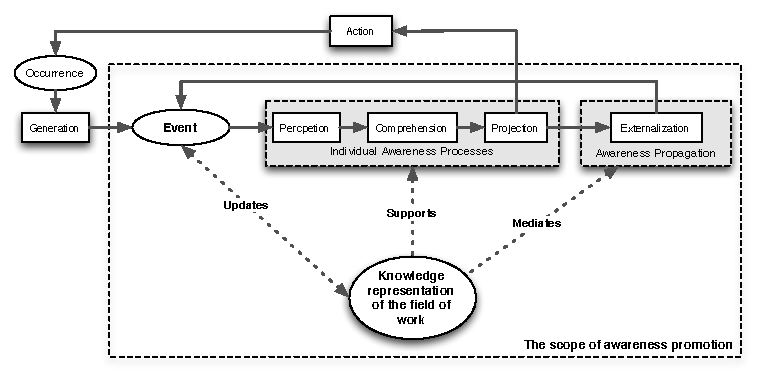
\includegraphics{awareness_promotion_framework.pdf} 
   \caption{Awareness promotion framework}
   \label{fig:awareness_promotion_framework}
\end{figure}

On one hand is how the computer constructs and develops the knowledge representation of the collaborative activities within the event-driven processes. In order to model the development of collaborative activities, the computational representation should support dynamic adaptation so that it always reflects the current state of the changing environment. As human actors use a subset of the awareness information to develop their individual awareness, the system processes the awareness information that is available in the whole collaborative activity. The awareness information can be generated by sensing the occurrences in real world, or it can be the results of human actors' externalization of their individual awareness. All of the awareness information will be processed by the computer system to update its knowledge representation of the collaborative activity.

On the other hand, the knowledge representation is used by the computer system to promote the awareness processes. In general, the promotion role of the computer system is to strike a balance between the system's reasoning capabilities and providing visual and interactive support. With the computational knowledge about the collaborative activities, the system can offload some of the reasoning effort from the human actors. Meanwhile, the systematic knowledge can also be visualized to help the human actors perform their part of the work. 

Following of this section discusses the major design choices of these two components, but leave the details to the next two chapters respectively.
% subsection the_awareness_promotion_framework (end)

\subsection{Computational knowledge representation} % (fold)
\label{sub:computational_knowledge_representation}
The nature of awareness phenomena in distributed, complex collaboration as we conceptualized in Section \ref{cha:the_conceptual_framework}, and the goal of promoting awareness impose several requirements for the knowledge representation of the collaborative activity:

\begin{enumerate}
   \item The knowledge representation should provides a precise model that can capture knowledge about all the three constructs in our conceptual model, i.e. the basic elements of human activities, the local scope of work for each actor, and the various dependency relationships among the actions. 
   \item The knowledge representation should be dynamically updated. Since the awareness needs of users change quickly with the development of collaborative activities, it is essential that the knowledge representation should be kept updating so that it always reflects the current state of the changing activities.
   \item The knowledge representation needs to be formalized and can be computationally modeled so as to support computational reasoning.
\end{enumerate}

Existing awareness systems have provided several approaches to representing the collaborative work. The AREA system \cite{fuchs1999a} describes the collaborative work as semantic networks including relationships among objects, where objects can be human actors artifacts, or aggregations such as groups of people. The representation is primarily used for the users to specify which objects and associated events they are interested in and when they want to be informed. The Atmosphere model \cite{Rittenbruch2002} describes the collaborative work as a hierarchically structured workspace that consists of a set of \emph{spheres} and \emph{sub-spheres}. Users classify their actions on artifacts by mapping them into different spheres. The MoMA model \cite{simone2002a} applies a reaction-diffusion metaphor to model the collaborative work as a set of entities embedded in an interaction space, which behave by using diffusion and reaction capabilities. This metaphor is based on the idea that whenever two or more entities have contact, their states are modified in some way. Their states are then propagated to others through fields in the space.  

Although these representations have shown their capabilities to support specific aspects of awareness in their respective application domains, none of them can meet all the three requirements for knowledge representation to enable awareness promotion. The AREA model provides a good representation of the activities and the dependencies using the semantic networks, but the local scopes of each user are not captured. The model is static (as it is pre-determined by the designers), and informal (as it is primarily used as a descriptive framework). The Atmosphere model organizes the field of work around the artifacts without explicit representation of activities. It supports the specification of each user's local scope using private `spheres', but no dependency relationships between activities are supported. It supports the modification to the representation by human users, but the system cannot automatically adapt the representation to changing environment. The MoMA model can support all the three constructs of the field of work as the definition of entities and spaces are generic, and provide some reasoning capabilities. However, it does not support the dynamical adaptation of the model.

In this study we draw knowledge representation and reasoning techniques from existing studies in artificial intelligence to develop a computational model of the collaborative activities that can satisfy all the three requirements. An important feature of our model is the capability to model intentions, beliefs, knowledge, and other attributes of actors' mental states \cite{grosz1996collaborative}. As human actors' awareness processes are directed by their mental models (Section \ref{ssub:individual_processes}), we believe that understanding and representing human actors' mental states allow the computer to infer each actor's local scope, and derive awareness needs from it. 
% subsection computational_knowledge_representation (end)

\subsection{Event driven awareness processes} % (fold)
\label{sub:event_driven_awareness_processes}
In our approach, we adopt the general event-driven interaction paradigm \cite{Etzion2010} to model the awareness processes. In an event-driven mode of interaction, actors (both human and computer) communicate by generating and receiving events. Each actor receives events from environment and other actors, reacts to them, and generates new events to other actors. We believe that the event-driven paradigm is suitable for modeling awareness processes in our study for two major reasons:

\begin{enumerate}
   \item The event-driven paradigm opens up the opportunities for active promotion by the computational system. Instead of asking the actors to monitor the environment and pull awareness information from it, events are pushed to the actors. This information push allows the system to take control and present the awareness information to the actors before they subscribe to them.
   \item As awareness information is explicitly represented as first-class objects in event-driven approaches, this allows for representing any aspects of the collaborative activities, not only the external aspects, but also the internal aspects reflecting the intentions and beliefs of the actors.
\end{enumerate}

Our event-driven model of awareness processes shares some commonality with existing event-based models, as both use events as the basic unit to organize and present awareness information. However, they also differ in several important ways:

\begin{enumerate}
   \item In existing event-based models, the computer primarily plays the role as producers of events. It detects events from sensors in the environment or feedbacks of human actions, filters them out based on user subscriptions, and present them to the users. However, in our approach, the computer is also the consumer of events. As to maintain the knowledge representation of the field of work, the computer needs to take the events as input of its reasoning process, and use them to make inference and update its knowledge representation. In this way, the computer behaves like other human actors to consume the events to develop its own awareness.
   \item The concept of events in our approach has a much richer meaning than existing event-based models. It is not only used to describe the occurrences in the environment and in human activities, but also the psychological experience of these occurrences as human actors perceive and interpret them. We make a clear distinction between real world occurrence, event, and awareness in Section \ref{ssub:the_concept_of_events}.
   \item Existing event-based models focus on the generation and presentation of events to the users, but our approach emphasizes the whole process of awareness development driven by events. This means we are not only concerned about how to select and present events to the users, but also how to support the interpretation of these events, and how new events are generated based upon existing ones.
   \item Existing event-based models treat the events as discrete from each other. The system processes one individual event each time. After the event is disseminated to the corresponding actors, the processing is done. However, as we conceptualize the awareness as undergoing continuous development, the events need to be considered as connected as they are built on top of each other.
\end{enumerate}

In sum, we consider the event not only as a way to represent awareness information, but also an effective interaction mode to drive the awareness development. In the following, we first clarify our concept of event, then describe the event-driven awareness processes. 

\subsubsection{The concept of event} % (fold)
\label{ssub:the_concept_of_events}
Before going further we should clarify what we mean by an event. The concept of the word `event' has been used in the literature from different perspectives:

\begin{enumerate}
   \item The first meaning refers to an actual occurrence (the something that has happened) in the real world. Set out by Quine \cite{quine1985events}, events in this meaning are first-class entities that can be localized in space and time, broken into sub-parts, and arranged in a taxonomic hierarchy. Research using this concept of events primarily focuses on studying the internal structures of the events. For example, in \cite{Yuan2001}, complex geographical phenomena, such as wildfire or precipitation, have been modeled in a hierarchy of events, processes, and states. In \cite{Andrienko2011}, the event-based approach has been adopted to model all the types of occurrences in movement analysis. The focus here is to derive the different event types that may occur and identify the relationships between them.
   \item The second meaning takes us into the realm of computerized event processing, where the word `event' is used to mean a programming entity that represents this occurrence \cite{Spiteri2000}. Each event in this notion is a message that describes an real world occurrence by its source, location, time, and other measurable properties. A single event occurrence can be represented by many event entities, and a given event entity might capture only some of the facets of a particular event occurrence \cite{Etzion2010}.
   \item In event-based awareness systems, the concept of event has a more specific meaning as representing a specific type of awareness information that might be relevant to the user's work. It is usually an application-specific concept, depending on the set of awareness information that is supported by an awareness system. For instance, the AREA system \cite{fuchs1999a} describes events as actions performed on an artifact and the event classes are derived from the artifact class hierarchy and possible operations on them. The ENI system \cite{Gross2004} describes events from the sensors associated with actors, shared artifacts, or any other objects that generate events related to them. 
\end{enumerate}

In this study, we use three different words to avoid the confusion when defining events:
\begin{enumerate}
   \item We use the word \emph{`occurrence'} to denote the real world happenings. It can be in the environment, e.g. the occurrence of a traffic accident at a location; or associated with an object, e.g. a vehicle arrives at the accident spot; or associated with human activities, e.g. the successful performance of first aid on a victim. 
   \item The word \emph{`awareness'} is used to refer to the human consciousness about the occurrences, events, and their relevance to ongoing or future human activities. It emphasizes that awareness is inherently a cognitive, interpretive, and predicative concept that reflects a state of mind.
   \item We use the word \emph{`event'} to denote a computerized entity that describes a piece of awareness information that is relevant to an actor's work. On one hand, it can be the description of a real world \emph{occurrence} by its measurable properties, e.g. the information about a traffic accident with time, location, number of victims etc. On the other hand, it can also be the externalization of an actor's \emph{awareness} knowledge, e.g. an actor's belief that the accident will block the traffic and cause a delay on delivery of medical team.
\end{enumerate}
% subsubsection the_concept_of_event (end)

\subsubsection{Awareness processes} % (fold)
\label{ssub:awareness_processes}
Along with the distinction between the concepts of \emph{`occurrence'}, \emph{`awareness'}, and \emph{`event'} is the notion of dynamic transformations between them (Figure \ref{fig:occurrence_event_awareness}). The transformations are tied to different processes in awareness development. 

\begin{figure}[htbp] %  figure placement: here, top, bottom, or page
   \centering
   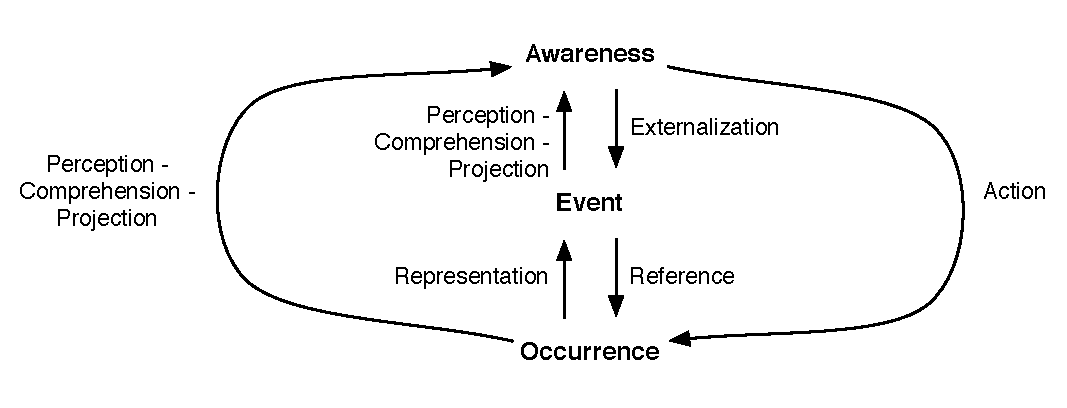
\includegraphics[width=4.5in]{occurrence_event_awareness.pdf} 
   \caption{Transformations between occurrence, event, and awareness}
   \label{fig:occurrence_event_awareness}
\end{figure}

The direct transformation between \emph{occurrence} and \emph{awareness} corresponds to the individual awareness development cycle that has been described in Section \ref{sub:awareness_as_process}. A real world \emph{occurrence} is transformed into \emph{awareness} through an actor's individual awareness processes, i.e. \emph{perception}, \emph{comprehension}, and \emph{projection}. Then, the achieved \emph{awareness} guides the actor's \emph{action} that may generate further \emph{occurrences} in the real world. 

The thing becomes more interesting when the computer support is involved and the transformations are driven by \emph{events}. One one hand is a real world \emph{occurrence} can be captured and represented as an \emph{event} by the computer system, and presented to a human actor. Instead of perceiving the \emph{occurrence} directly, the actor perceives the corresponding \emph{event} in the computer interface, and develops the \emph{awareness} upon it through the actor's individual awareness processes, i.e. \emph{perception}, \emph{comprehension}, and \emph{projection}. On the other hand is some aspect of the actor's \emph{awareness} can be externalized as a new \emph{event}, which refers to some current \emph{occurrence} or predicts future \emph{occurrence} in the real world.

The event-driven transformations can also be used to describe the different types of awareness transactions across multiple actors. The process of \emph{mutual monitoring} can then be described in the following steps: (1) an actor's \emph{awareness} guides his/her \emph{action} that generates a new \emph{occurrence} in the real world; (2) this new \emph{occurrence} is then captured and represented as an \emph{event} by the computer, and presented to another actor; (3) the other actor develops the \emph{awareness} upon receiving the new event. Similarly, the process of \emph{externalization} can also be described as follow: (1) an actor's \emph{awareness} is externalized as a new \emph{event}, which refers to some current \emph{occurrence}; (2) this new \emph{event} is then presented to another actor by the computer; (3)the other actor develops the \emph{awareness} upon receiving the new event. 

Figure \ref{fig:example_awareness_traj} shows an example of how these event-driven awareness processes can be combined together to describe a developmental trajectory of awareness that involves three actors in a group. The awareness is propagated from $Actor1$ to $Actor2$ through the process of \emph{externaliation}, and is then propagated from $Actor2$ to $Actor3$ through the process of \emph{mutual monitoring}.

\begin{figure}[htbp] %  figure placement: here, top, bottom, or page
   \centering
   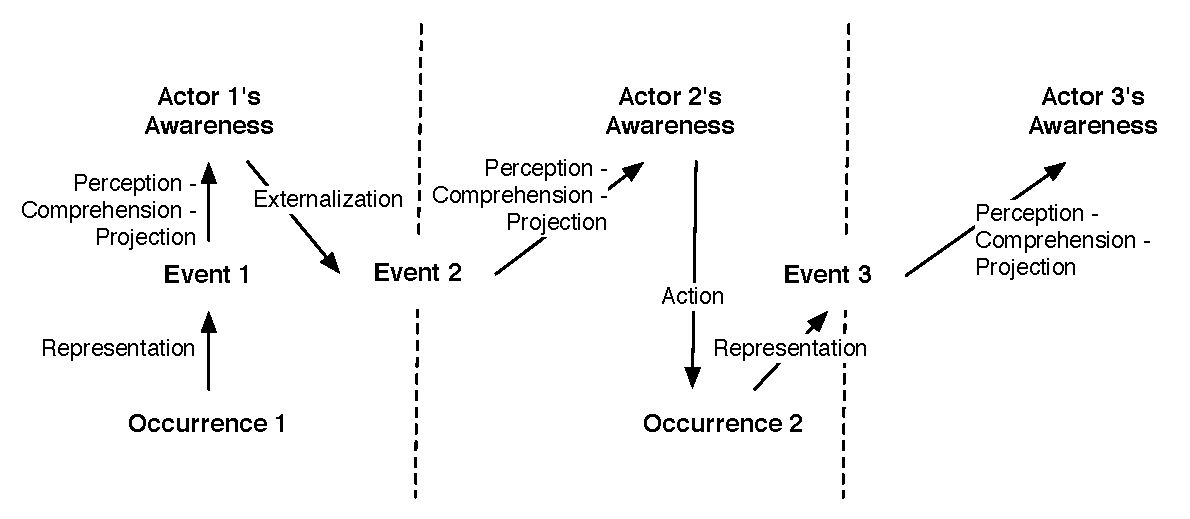
\includegraphics[width=4.5in]{example_awareness_traj.pdf} 
   \caption{An example of event-driven developmental trajectory}
   \label{fig:example_awareness_traj}
\end{figure}
% subsubsection awareness_processes (end)
% subsection event_driven_awareness_processes (end)
% section awareness_promotion_approach (end)

\section{Discussion} % (fold)
\label{sec:discussion}
In this chapter, we first identify the major challenges for human actors to achieve and develop awareness in distributed, complex collaborative activities, which highlight the design aspects in which computer systems can provide support to augment and complement human capability at both the individual and team levels. 

The analysis of the design aspects provide us the basis to review existing awareness support systems. The purpose of the review, however, is not to provide an exhaustive evaluation on existing studies. Instead, we use the review to understand how the design aspects have been addressed or partially addressed in existing awareness support systems, and identify the major limitations:

\begin{enumerate}
   \item Existing systems to support awareness processes are usually designed to support collaborative activities at relatively small and medium scales, it becomes a much more difficult task to support awareness in large-scale distributed activities as we are interested in this study. One one hand, space-based models rely on the users to monitor the shared spaces and perceive the awareness information. This provides more flexibility to handle increased level of dynamics, but at the same time it becomes  problematic when the collaborative is scaled up with higher level of complexity and actions of users are highly distributed. On the other hand, event-based systems are more efficient to handle higher-level of complexity as the users can decide on what aspects of awareness information that should be presented, and they do not need to switch their attentions to other’s actions until the event notification happens. However, event-based systems become less effective in high level of dynamics as the user's awareness needs are often in the flux of changes.
   \item The support for various awareness processes at both the individual and collaborative levels are limited. At the individual level, existing awareness systems have focused on supporting perception, the higher level of awareness processes are relatively less supported. At the team level, existing awareness systems have focused on either supporting the explicit communication among human collaborators, or different approaches to providing ‘shared spaces’ so that the actions of each other become visible to each other. However, less discussion has been given to support explicit representation of transactive knowledge, or the externalization process.
\end{enumerate}

Motivated by these limitations, we argue that the computer system needs to play a more active role to promote awareness among collaborators, and provide an overview the awareness promotion approach. We believe the characteristics of awareness promotion approach provide the potential to address limitations of existing awareness systems to handle the scaled up complexity and dynamics, and to provide integrated awareness support. First, the awareness promotion approach utilizes the computational knowledge representation to model the collaborative activities and offloads some of the representation and reasoning efforts from the human to the computer. Hence, it can  handle more complex collaborative configurations than existing awareness models. Meanwhile, the knowledge representation is dynamically updated to reflect the current state of the collaborative work, which allows it to handle increased level of dynamics. Last, as the computer's knowledge representation is at the team level and is equipped with the computational reasoning capabilities, it allows the computer to provide support on both the higher level of individual awareness processes and awareness transactions.

The next two chapters provide details of this awareness promotion framework. Chapter \ref{cha:knowledge_reprsentation_and_updating} describes the knowledge components, i.e. the computational representation of the collaborative activities and the specification of events, and the mechanisms for updating the knowledge representation with events. Chapter \ref{cha:promoting_event_driven_awareness} describes the different promotion strategies making sue of the knowledge representation.
% section discussion (end)
% chapter awareness_promotion (end)



 


%!TEX root = ../BoYu-Dissertation.tex
\graphicspath{{Figures/}}

\chapter{Knowledge Representation and Updating} % (fold)
\label{cha:knowledge_reprsentation_and_updating}
In this chapter, we provide details about the first component of our computational framework for event-driven awareness promotion, i.e. how the computer constructs and develops the knowledge representation of collaborative activities within the event-driven processes. We first provide a computational representation of collaborative activities using the PlanGraph model. Then, we discuss the specification and typology of events in our approach. Based on these two knowledge components, we discuss the the knowledge updating process, in which they are mutually developed. On one hand, the knowledge representation of an collaborative activity is updated by reacting to the various external and internal events, so that it always reflects the current state of the collaborative activity. On the other hand, during the updating process, the system's knowledge about the events are also enriched by interpreting their meanings in the context of the collaborative activity.

\section{Representing collaborative activities} % (fold)
\label{sec:representing_the_field_of_work}
In this section, we present the knowledge representation of collaborative activities based on PlanGraph model. By modeling an collaborative activity within a PlanGraph, the various entities and relations as we formalized in Section \ref{sub:structure_of_a_collaborative_activity} can be represented as different components of the PlanGraph. Then we show how the local scopes and dependency networks can be derived from the PlanGraph model, making use of the knowledge about these entities and relations.

\subsection{The PlanGraph model} % (fold)
\label{sub:the_plangraph_model}
The PlanGraph model with its basis in the SharedPlans theory is designed to represent the dynamic knowledge in the human-computer collaboration \cite{Cai2005}. In general, a PlanGraph represents the knowledge about a collaborative activity towards a shared goal in a hierarchical way (Figure \ref{fig:plangraph}). The root of a PlanGraph is the overall goal of the actors in a collaborative activity, which is decomposed recursively into actions through the adoption of recipes. The PlanGraph as a whole represents the shared plan corresponding to the top-level collaborative activity, while each sub-tree with an action as the root represents the shared plan for that action. A PlanGraph is composed of three types of nodes: (1) \emph{action} nodes represent all the actions and sub-actions in the collaborative activity; (2) \emph{parameter} nodes represent informational or physical objects that are used by actions; (3) \emph{condition} nodes represent states of affairs in the world that the actors would like to achieve.

There are several ways that these three types of nodes can be connected in a PlanGraph:
\begin{enumerate}
	\item An action can be decomposed into several parameters, conditions, and sub-actions, where the parameters indicate all the informational or physical objects that will be used by the action. All these parameters need to satisfy their own constraints before the action can be performed, and they are accessible by all the subsidiary actions at the same level. The conditions under an action correspond to all the constraints that need to be satisfied before the action or any sub-actions can be performed.  
	\item Each parameter can be decomposed into sub-actions and conditions. The sub-actions of a parameter are used to assign values for the parameter, i.e. they are used to satisfy the knowledge-precondition on the parameter. The conditions attached to a parameter are other preconditions that need to be satisfied before the parameter is ready to be used by upper action.
	\item Each condition can only be decomposed into subsidiary actions that are used to ensure the condition is satisfied.
\end{enumerate}

The PlanGraph model also encodes the actors that are participated in each action. Because the relations between actors and actions can be many-to-many, i.e. an actor can work on multiple actions, and one action can involve multiple actors, we represent knowledge of actors within their relations towards each action. Each action node in a PlanGraph includes several attributes to store the relations with participating actors as defined in Section \ref{ssub:relations}: \emph{Intentions} records the different intention relations of each actor towards the action. \emph{Capabilities} indicates the level of capability of each actor to perform the action.

\begin{figure}[htbp] %  figure placement: here, top, bottom, or page
   \centering
   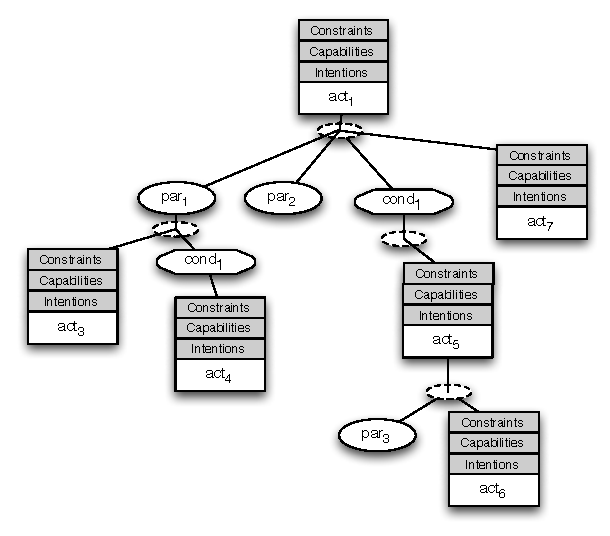
\includegraphics{plangraph.pdf} 
   \caption{Structure of a PlanGraph}
   \label{fig:plangraph}
\end{figure}

The PlanGraph model has been used to model the human-computer collaboration as a collaborative activity in several applications, e.g. the natural conversational interface to geospatial databases \cite{Cai2005}, collaborative dialog-based system to communicate vague spatial concepts \cite{Cai2003}, and context-aware mobile mapping \cite{yu2010using}. However, in order to model the collaborative activities among human actors, several modifications to the original PlanGraph model have been made in this study:

\begin{enumerate}
 	\item First, the parameter nodes in the original PlanGraph model are mainly used to represent knowledge preconditions, i.e. they represent the knowledge needed for the action to be performed. In this study, we extend the concept of parameter to represent both the physical and informational resources that are needed for the action.
 	\item We extend the original PlanGraph model to explicitly represent conditions as standalone nodes. This allows us to model the indirect dependency relations among actions between human actors. For instance, even though $act_1$ does not indicate a higher level goal of $act_2$, it can still depends on the $act_2$ because $act_2$ satisfies a condition that is required for performing $act_1$.
 	\item The original PlanGraph model for human-computer collaboration treats the computer system as an actor with its own intentions and beliefs. However, as we focus on tracking the states and relations among human actors' actions, we do not explicitly model the computer's beliefs and intentions.
 \end{enumerate} 
% subsection the_plangraph_model (end)

\subsection{Representing elements and relations} % (fold)
\label{sub:representing_activities}
The PlanGraph model allows us to represent the basic entities and relations in a collaborative activity. The actions, actors, and resources are first-class objects in the PlanGraph model, and the multiple relations among then can be represented as structural relations in the PlanGraph model (Table \ref{tab:basic_rel_pg}). 

\paragraph*{Actors} % (fold)
\label{par:actors_in_plangraph}
Each actor is represented as an object with a unique \emph{ID} in the PlanGraph model. Each actor object in the PlanGraph maintain the current state of the corresponding actor, such as the name, the location, the role of the actor, and the expertise he/she has. Each actor object also maintains a list of actions that the actor is currently participated in.
% paragraph actors_in_plangraph (end)

\paragraph*{Actions} % (fold)
\label{par:actions_in_plangraph}
Actions are directly modeled as a type of nodes in the hierarchical structure of the PlanGraph. Each action node has several important attributes:
\begin{enumerate}
	\item The \emph{goal} of the action is represented as an expression, indicating the expected effect of the action when it is successfully performed.
	\item The \emph{execution state} of the action records the current state of the action towards its performance, e.g. whether it has been started, successfully performed, or in the progress.
	\item The \emph{recipe} points to the current recipe to perform the action if the current recipe is selected from the knowledge base. Each recipe specifies a particular way to perform the action. In the case the recipe is identified by human actors on the fly, this could be empty.
	\item The \emph{Intentions} and \emph{Capabilities} record the different relations between participating actor towards the action.
	\item The \emph{Constraints} record the relations between sub-actions, such as temporal orders between them, or whether they can be optional.
\end{enumerate}
% paragraph actions_in_plangraph (end)

\paragraph*{Resources} % (fold)
\label{par:resources_in_plangraph}
Resources are assigned to parameter nodes as values. Parameter nodes can be collective or individual. A collective parameter includes a collection of resources with the same type as its value, for instance, a parameter representing all the victims in the same rescue operation. All the resources assigned to the same parameter node need to satisfy conditions that are linked to the resource node.
% paragraph resources_in_plangraph (end)

\paragraph*{Relations between actors and their actions} % (fold)
\label{par:relations_between_actors_and_their_actions}
The relations between actors and their actions can be directly retrieved from the \emph{Intentions} and \emph{Capabilities} attributes attached to each action, recording the different relations between participating actors towards the action.
% paragraph relations_between_actors_and_their_actions (end)

\paragraph*{Relations between actions} % (fold)
\label{par:relations_between_actions}
The two major types of relations between actions are composition and precedence. The former is directly encoded in the hierarchical structure of a PlanGraph. Each action node has an list of its sub-actions under current plan. The precedence relation that reflects the temporal order of performing two actions is encoded in the \emph{constraints} attribute of their parent action node.
% paragraph relations_between_actions (end)

\paragraph*{Relations between resources and actions} % (fold)
\label{par:relations_between_resources_and_actions}
The relations between resources and actions can be inferred from the structural relations between action nodes and parameter nodes in a PlanGraph. The resources assigned to a parameter node underlying an action node can be consumed by the action and all its sub-actions. The actions that are used to assign values to a parameter or achieve preconditions of the parameter can manipulate all the resources attached to the parameter node.
% paragraph relations_between_resources_and_actions (end)

{\footnotesize
\begin{longtable}{>{\raggedright}p{1.5in}>{\raggedright}p{4in}}
\toprule 
Relation & Structure in PlanGraph\tabularnewline
\midrule 
$Pot.Int(ar,act)$ \par $Int.Th(ar,act)$ \par $Int.to(ar,act)$ \par $Perform(ar,act)$ & search the \emph{Intentions} slot attached to each action node: 
\par 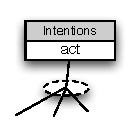
\includegraphics{intentions.pdf}\tabularnewline
\midrule 
$Knows(ar,act)$ \par $Able(ar,act)$ \par $Workable(ar,act)$ & search the \emph{Capability} slot attached to each action node: 
\par 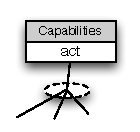
\includegraphics{capabilities.pdf}\tabularnewline
\midrule 
$Sub.Act(act_1, act_2)$ &  $act_1$ is a subsidiary action node under $act_2$: 
\par 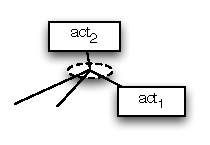
\includegraphics{sub_act.pdf} \tabularnewline
\midrule 
$Precedes(act_1, act_2)$ &  $act_1$ and $act_2$ as ordered siblings: 
\par 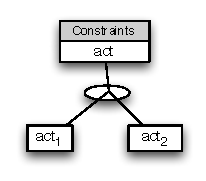
\includegraphics{precedes.pdf}\tabularnewline
\midrule 
$Consume(act, res)$ & a parameter node representing a resource $res$ and  a action node $act$ as siblings: 
\par 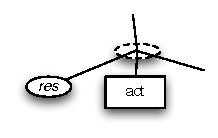
\includegraphics{consumes.pdf}\tabularnewline
\midrule 
$Produces(act, res)$ &  $act$ is a subsidiary action node under the parameter node representing a resource $res$: 
\par 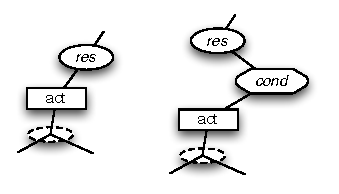
\includegraphics{produces.pdf}\tabularnewline
\bottomrule
\caption{Representing basic relations in PlanGraph}
\label{tab:basic_rel_pg}
\end{longtable}
}
% subsubsection representing_relations (end)
% subsection representing_activities (end)

\subsection{Constructing local scopes} % (fold)
\label{sub:representing_local_scopes}
Based on the definition of local scopes in Section \ref{sub:local_scope_of_work}, the local scope of an actor can be dynamically constructed by depth-first traversal through the PlanGraph structure to search for all the actions that are related to the actor through intention or capability relations.

We define a procedure $BUILD\textrm{-}LS$ that takes an actor object $ar$ and a PlanGraph $PG$ to construct both the local scope of intentions $LSI$ and local scope of capabilities $LSC$ for the actor. We define a sub-procedure $ADD\textrm{-}To\textrm{-}LS$ that takes an actor object $ar$ and an action node $act$ in the PlanGraph to add the action to the local scope $LSI$ or $LSC$ based on whether the corresponding intention or capability relation exists. The $ADD\textrm{-}TO\textrm{-}LS$ procedure then calls itself recursively on all the children nodes to traverse to the deeper levels in the PlanGraph. In this way, the process to construct the local scopes $BUILD\textrm{-}LS$ starts with the initialization of $LSI$ and $LSC$, and then recursively calls $ADD\textrm{-}TO\textrm{-}LS$ from the root node of the PlanGraph.

{\footnotesize
\begin{algorithm}
\begin{algorithmic}[1]
\Procedure{BUILD-LS}{$ar,PG$}
	\State $LSI\gets [\:], LSC\gets [\:]$
	\State $root\gets PG.root$
	\State $ADD\textrm{-}TO\textrm{-}LS(ar, root)$\Comment{start the recursion from $root$}
\EndProcedure
\Procedure{ADD-TO-LS}{$ar,act$}
	\ForAll{$int$ \textbf{in} $act.intentions$}\Comment{check the current node}
   		\If{$int.actor == ar$}
   			\State $LSI.add(ar, act, int)$
   		\EndIf
	\EndFor
	\ForAll{$cap$ \textbf{in} $act.capabilities$}
   		\If{$cap.actor == ar$}
   			\State $LSC.add(ar, act, cap)$
   		\EndIf
	\EndFor
	\ForAll{$par$ \textbf{in} $act.parameters$}\Comment{recursion on parameters}
   		\ForAll{$subact$ \textbf{in} $par.subacts$}
   			\State $ADD\textrm{-}TO\textrm{-}LS(ar, subact)$
		\EndFor
	\EndFor
	\ForAll{$cond$ \textbf{in} $act.conditions$}\Comment{recursion on conditions}
   		\ForAll{$subact$ \textbf{in} $cond.subacts$}
   			\State $ADD\textrm{-}TO\textrm{-}LS(ar, subact)$
		\EndFor
	\EndFor
	\ForAll{$subact$ \textbf{in} $act.subacts$}\Comment{recursion on subacts}
   		\State $ADD\textrm{-}TO\textrm{-}LS(ar, subact)$
	\EndFor
\EndProcedure
\end{algorithmic}
\end{algorithm}
}
% subsection representing_local_scopes (end)

\subsection{Constructing dependency network} % (fold)
\label{sub:representing_dependencies}
From the PlanGraph model, we can also dynamically construct the corresponding dependency network to represent how the actions are dependent on each other. Formally, a dependency network $DN=(V(DN), E(DN))$ is defined as a directed graph with the following characteristics:
\begin{enumerate}
	\item $V(DN)=\{ACT \cup PARAM \cup COND\}$ is the set of all the nodes in the dependency network, all the \emph{dependers} and \emph{dependees} are action nodes $ACT$, and the \emph{dependums} can be any parameter $RES$ or condition nodes $COND$. 
	\item The set $E(DN)$ is a set of links between the nodes. Each link can be represented as a pair of nodes in $V(DN)$, i.e. $E(DN) \to V(DN) \times V(DN)$. The link can indicate a direct dependency between two action nodes, or a incoming link that connects a \emph{depender} and \emph{dependum}, or an outgoing link that connects a \emph{dependum} and \emph{dependee}.
\end{enumerate}

The construction of dependency network can also be achieved by depth-first traversal through the PlanGraph model to search for all the action-action and action-resource relations. We define a procedure $BUILD\textrm{-}DN$ that constructs a dependency network from a PlanGraph $PG$. As the set of nodes $V(DN)$ can be calculated from the set of links $E(DN)$ by removing all the duplicates, the $BUILD\textrm{-}DN$ procedure focuses on building $E(DN)$. We define a sub-procedure $ADD\textrm{-}To\textrm{-}DN$ that takes an action node $act$ in the PlanGraph to add dependencies that starting from $act$, i.e. to find all the dependencies in which the $act$ is the \emph{depender}.

{\footnotesize
\begin{algorithm}
\begin{algorithmic}[1]
\Procedure{BUILD-DN}{$PG$}
	\State $E\gets [\:]$
	\State $root\gets PG.root$
	\State $ADD\textrm{-}TO\textrm{-}DN(root)$\Comment{start the recursion from $root$}
\EndProcedure
\Procedure{ADD-TO-DN}{$act$}
	\ForAll{$subact$ \textbf{in} $act.subacts$}\Comment{check for Sub.Act}
   		\State $E.add(act, subact)$
	\EndFor

	\If{$act.hasParent()$}
		\ForAll{$constr$ \textbf{in} $act.parent.constraints$}\Comment{check for Precedes}
			\If{$constr.next == act$}
   				\State $E.add(act, constr.prev)$ 
   			\EndIf
		\EndFor
		\ForAll{$par$ \textbf{in} $act.parent.parameters$}\Comment{check for parameters}
   			\ForAll{$subact$ \textbf{in} $par.subacts$}
   				\State $E.add(act, par), E.add(par, subact)$
			\EndFor
		\EndFor
		\ForAll{$cond$ \textbf{in} $act.parent.conditions$}\Comment{check for conditions}
   			\ForAll{$subact$ \textbf{in} $cond.subacts$}
   				\State $E.add(act, cond), E.add(cond, subact)$
			\EndFor
		\EndFor
   	\EndIf

	\ForAll{$par$ \textbf{in} $act.parameters$}\Comment{recursion on parameters}
   		\ForAll{$subact$ \textbf{in} $par.subacts$}
   			\State $ADD\textrm{-}TO\textrm{-}DN(subact)$
		\EndFor
	\EndFor
	\ForAll{$cond$ \textbf{in} $act.conditions$}\Comment{recursion on conditions}
   		\ForAll{$subact$ \textbf{in} $cond.subacts$}
   			\State $ADD\textrm{-}TO\textrm{-}DN(subact)$
		\EndFor
	\EndFor
	\ForAll{$subact$ \textbf{in} $act.subacts$}\Comment{recursion on subacts}
   		\State $ADD\textrm{-}TO\textrm{-}DN(subact)$
	\EndFor
\EndProcedure
\end{algorithmic}
\end{algorithm}
}
% subsection dependency_relations_in_the_activity_structure (end)
% section representing_the_field_of_work (end)

\section{Representing events} % (fold)
\label{sec:representing_events}
In Section \ref{ssub:the_concept_of_events}, we define \emph{`events'} to refer to the computerized entities that are used in an awareness system to represent knowledge about either real world \emph{`occurrence'} or the results of \emph{`awareness'} processes. In this section, we focus on how events are computationally represented in this study. Although they share the same representational structure in general, different types of events are represented differently. In the following, we first describe the general representational structure of events, then discuss the major event types, and their differences in representation.

\subsection{Structure of events} % (fold)
\label{sub:defining_events}
We follow many existing event processing systems to represent each event as a structured object consisting of a named set of attributes \cite{Mhl2010}. Formally, an event $e$ is a nonempty set of \emph{attributes} $\{a_1, a_2, ..., a_n\}$, where each $a_i$ a name/value pair $(n_i, v_i)$ with name $n_i$ and value $v_i$. It is assumed that names are unique, i.e., $i\ne j \Rightarrow n_i\ne n_j$, and that there exists a function that uniquely maps each $n_i$ to a data type $T_i$ that is the type of the corresponding value $v_i$.

The set of attributes for each event should help answer questions such as: What occurrence or awareness aspect it refers to? When did it happen? Where did it happen? What other information is associated with its happening? The answers to these questions are usually depend on the type of event they are associated with. An \emph{event type} is a generalization for a set of event objects that have the same semantic intent and same structure \cite{Etzion2010}, i.e. they share the same set of attributes, but may have different values. Each \emph{event type} has a unique event type identifier. In this study we use simple descriptive text strings for these identifiers, for example the phrase \emph{``LocationChanged''} identifies an event type that can describe any instance of an object's location change. Identifying the set of \emph{event types} is an application specific task, as actors in different applications have different awareness needs and capabilities to detect events. We describe the major event types that are supported in this study in Section \ref{sub:event_types}.

While arbitrary attributes can be included in each event type, we can group them into three categories, following the definitions in \cite{Etzion2010} (Figure \ref{fig:event_structure}):

\begin{enumerate}
	\item The \emph{header} consists of generic information about the event, such as the event type, occurrence time, etc. The header attributes are not specific to a particular event type, rather shared by all event types.
	\item The \emph{payload} contains a collection of attributes carrying the data that describes the actual occurrence. Unlike header attributes independent of the actual event type, the payload attributes are defined per event type. 
	\item An event can also contain free-format \emph{open content} information that provides a mechanism that the awareness system can use to enrich an event object with extra contextual information, such as human-readable explanation, multi-media content etc.
\end{enumerate}

\begin{figure}[htbp] %  figure placement: here, top, bottom, or page
   \centering
   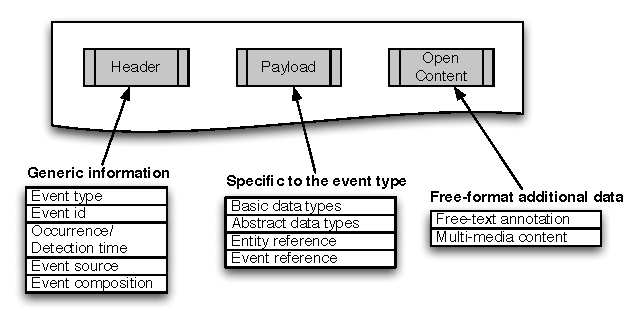
\includegraphics{event_structure.pdf} 
   \caption{The structure of an event (adapted from \cite{Etzion2010} p.63)}
   \label{fig:event_structure}
\end{figure}

\paragraph*{Header} % (fold)
\label{par:header}
The header of an event contains the common attributes that are included in every event object. Unlike payload or open content that are optional, a header is required for every event representation. In general, the header of an event needs to include the following attributes:

\begin{enumerate}
	\item \emph{Event type}. This attributes stores the event type identifier that uniquely identifies the event type of this event.
	\item \emph{Event identifier}. This is a unique identifier for each individual event object.
	\item \emph{Occurrence/detection time}. The occurrence time is the time when the real world occurrence happens. In some cases, the event producer might not be able to determine the time when the event actually occurred. For example, if the producer examines the state of some external entity only at periodic intervals. In such cases, the detection time is used instead, recording the time at which the event became known by the event producer. 
	\item \emph{Event source}. This is the entity that originates this event. This can be either an external sensor, or a human actor in the collaborative system.
	\item \emph{Event composition}. This is a boolean attribute that denotes whether the specific event is a composite event or not. A composite event is one whose payload is made up of several other event instances.
\end{enumerate}
% paragraph header (end)

\paragraph*{Payload} % (fold)
\label{par:payload}
The attributes that make up the event payload are used to carry the data that describes the actual occurrence. The set of attributes included in each event is a variable that depends on the corresponding event type. There are several types of data that can be included as payload attributes:
\begin{enumerate}
	\item \emph{Basic data types}. The value in an payload attribute can simply be in the basic data types, such as string, numeric boolean, date/time etc.
	\item \emph{Abstract data types}. Attributes can also have abstract data types that are structures composed of other data types. For example, many events includes a geographic attribute to records the whereabout of the represented real world occurrence. This attribute can be a point-based representation as a latitude/longitude pair, or more complicated as a route or a geographic area.
	\item \emph{Entity reference}. Instead of records the information directly in an attribute, the event can also records information by pointing to entities represented in the collaborative activities. For example, an \emph{`ActionPerformed'} event may use the reference to the action node stored in the PlanGraph model to indicate which action has been performed.
	\item \emph{Event reference}. Some events may contain references to other events. For example, a composite event may use the event references to record the primitive events that it is composed of.
\end{enumerate}
% paragraph payload (end)

\paragraph*{Open content} % (fold)
\label{par:open_content}
The open content of an event can include any attributes an awareness system can use to provide additional contextual information about the event. For example, it is used in the awareness externalization process to allow the actors to provide human-readable explanation of their interpretations.
% paragraph open_content (end)

% subsection defining_events (end)
\subsection{Event types} % (fold)
\label{sub:event_types}
As we argue in Section \ref{ssub:the_concept_of_events} that \emph{events} can be used to represent both description of real world \emph{occurrences} and externalization of human actors' internal \emph{awareness} knowledge, a fundamental distinction should be made between these two categories of events, we call the former \emph{external events}, and the latter {internal events}. The distinction between external events and internal events are important, because (1) they require different representational structures, i.e. the payloads of events have different sets of attributes; (2) they are consumed differently by the system when updating the knowledge representation; (3) and they are treated differently in  human users' awareness processes as well. 

Another distinction to make is the difference between \emph{primitive events} and \emph{composite events}. Composite events prevent the users from being overwhelmed by a large number of primitive event by providing them a higher-level abstraction \cite{Mhl2010}. Generally, a composite event is made up of several other events (either primitive or composite), according to a specification of relations between them. 

In the following, we first describe the major primitive event types, both external and internal, and then discuss the composite events as a special event type with its own payload structure.

\subsubsection{External events} % (fold)
\label{ssub:external_events}
As we conceptualize a collaborative environment as consisting of a variety of entities and relations, external events can be defined to indicate any kinds of changes on either these entities or relations. 

\paragraph*{Events on entities} % (fold)
\label{par:events_on_entities_}
We define each external event on an individual entity as a semantic function that changes the entity's property or state. We follow the general event ontology proposed in \cite{Kaneiwa2007} to define the following categories of external events on individual entities:

\begin{enumerate}
	\item \emph{State Change}. An event is a state change event if the occurrence yields a change of state on an entity. All the possible states of an entity are usually can be expressed as a discrete state machine, and each state transition indicates a possible state change event. For example, Figure \ref{fig:action_exec_state_trans} shows the transition diagram with all the possible execution states of an action. Each valid transition in the diagram can be considered as a state change event.
	\begin{figure}[htbp] %  figure placement: here, top, bottom, or page
   	\centering
   	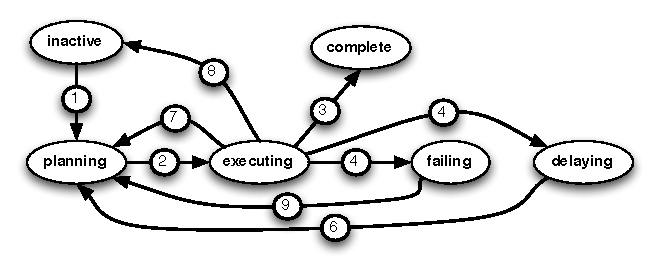
\includegraphics{action_exec_state_trans.pdf} 
   	\caption{Execution state transition of an action}
   	\label{fig:action_exec_state_trans}
	\end{figure}
	\item \emph{Existential Change over Time}. An event indicates an existential change over time if its occurrence changes the existence of an entity in temporal order, e.g. an entity did not exist in the past but it exists now.
	\item \emph{Existential Change over Space}. An event indicates an existential change over space if its occurrence changes the existence of an entity depending on its movement through space, e.g. an entity existed at location A, but now exists at location B. 
	\item \emph{Value Comparison}. Another common class of external events are comparison events to indicate changes on attribute values of an entity. They can used to indicate whether an attribute value is equal, unequal, greater than, or less than a fixed threshold, or the same attribute value in the past. 
\end{enumerate}
% paragraph events_on_entities_ (end)

\paragraph*{Events on relations} % (fold)
\label{par:events_on_relations}
Events on relations are used to indicate whether some relations between entities hold. For example, an event with the type \emph{`ResourceAssigned'} indicates an assignment relation between a resource and an action becomes holding, i.e. the resource is now assigned for performing the action. Therefore, the types of external events on relations depend on the possible types of relations that can be identified in the domain. 

Generally, the basic relations between entities in the real world can be divided into three categories: spatial, temporal, and conceptual \cite{Tomaszewski2010}.

\begin{enumerate}
	\item The spatial relations link the entities through their spatial positions. The basic types of spatial relations have been well studied in the literature of geographic information systems, include binary topological \cite{egenhofer1994deriving}, directional \cite{frank1991qualitative}, and distance relations \cite{hernandez1995qualitative}. Topological relations is a particular subset of geometric relations that are preserved under topological transformations such as translation, rotation, and scaling. Some examples are relations indicating whether one entity disjoints, meets, overlaps, or contains another entity. Directional relations indicate the relative direction between two entities, such as one is at north of the other. Distance relations link entities based on their proximity in the space, such as one is within a certain range of another. 
	\item The temporal relations link the entities based on their temporal positions. The basic types of temporal relations are considered in the literature on temporal reasoning \cite{allen1994actions}, including binary topological, ordering, and distance relations \cite{Andrienko2011}.
	\item The conceptual relations are an umbrella term that covers all the different types of organizational, structural, or social relations between entities in a particular collaborative activity. 
\end{enumerate}

From the basic types of relations, more complex types of relations can be built, such as
density (clustering, dispersion), arrangement (e.g. sequence in time or alignment in space) and spatial-temporal relations. The latter are composed of spatial and temporal relations and represent changes of spatial relations over time: approaching or going away, entering or exiting, following, keeping distance, concentrating or dissipating and so on.
% paragraph events_on_relations (end)

Figure \ref{fig:external_events} shows an upper level typology of the external events that can be defined on entities and relations in a collaborative environment.
\begin{figure}[htbp] %  figure placement: here, top, bottom, or page
	\centering
	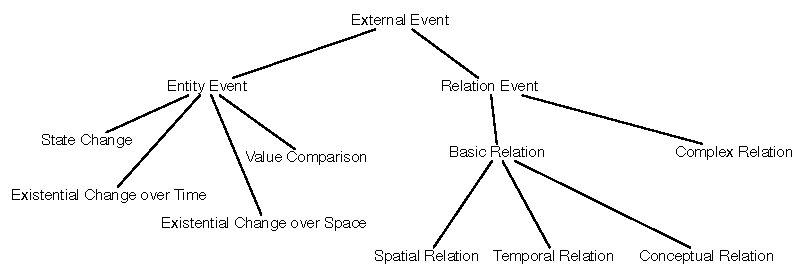
\includegraphics{external_events.pdf} 
	\caption{An upper level typology of external events}
	\label{fig:external_events}
\end{figure}

\paragraph*{Relevance to the collaborative activities} % (fold)
\label{par:relevance_to_the_field_of_work}
 Although the number of external events that could be possibly identified is infinite, not all of them are relevant to the human actors' working context. As a result, the goal of identifying external events in an awareness system focuses on finding a subset of event types that could possibly contribute to the understanding of supported collaborative activities. In general, we believe that the relevance of external events to a collaborative activity can be analyzed based on the different functional roles they can play in updating the knowledge about the collaborative activity. If the occurrence of an external event can imply some change in the collaborative activity, it should be treated as relevant. Based on our conceptualization of collaborative activities, we can identify the following function roles for external events:

 \begin{enumerate}
 	\item \emph{Direct change to entities in a collaborative activity}. External events can indicate changes on individual entities that are modeled in a collaborative activity, i.e. the property or state change of the resources, actors, or actions. For example, a state change event can be used to indicate the change of execution state for an action. Location change events can be used to describe an actor's movement. 
 	\item \emph{Direct change to relations in a collaborative activity}. Some external events are directly related to the various relations between resource, actors, and actions as we described in Section \ref{ssub:relations}. For example, an external event type indicating the constitution relation between two entities can be used to describe the $Sub.Act$ relation between two actions, i.e. one action is a subsidiary action to perform another one. The assignment relation event type can be used to describe relations between an action and a resource, i.e. the resource has been assigned to the performance of the action. 
 	\item \emph{Goal activation}. Aside from the two cases that external events can be directly linked to the entities and relations in a collaborative activity, external events can also impact the collaborative activity by activate the goals to perform actions. For example, an external event indicating that the fire alarm is ringing will activate the human actor's goal to escape from the office. In this case, the fire alarm is not directly linked to any entities in the human actor's activities, rather it motivates the actor to perform a new action.
 	\item \emph{Implied changes to entities and relations}. In some cases, external events can also provide some evidence implying changes in the entities and relations in a collaborative activity. For example, instead of a state change event directly showing the action to delivery a resource to an actor has been completed, it could be implicitly inferred from a spatial relation event that indicates the resource is now located at the actor's location. Similarly, an external event indicating the occurrence of a traffic blocking between the resource's current location and the actor's implies the delivery action is in trouble.
 \end{enumerate}
% paragraph relevance_to_the_field_of_work (end)
% subsubsection external_events (end)
\subsubsection{Internal events} % (fold)
\label{ssub:internal_events}
Internal events are used to describe the results of human actors' awareness processes. Unlike external events that can describe changes in any entities and relations in a collaborative activity, internal events describe the changes of human actors' internal mental states towards the collaborative activity. Internal events are usually derived from external events to indicate human actors' interpretations on them. In this study, we identify two types of internal events: \emph{intention} events and \emph{belief} events. 

An \emph{intention} event indicates a human actor's adoption of certain intention towards some action in a collaborative activity. Figure \ref{fig:intention_event} shows the basic structure of an intention event. The payload of an intention event include three required attributes: an intention type indicating whether it's $Pot.Int$, $Int.Th$, or $Int.To$, a reference to the actor who adopts this intention, and a reference to the intended action. An optional free-text attribute is included in the open content part, where the human actor can provide the rationale for adopting the corresponding intention.
\begin{figure}[htbp] %  figure placement: here, top, bottom, or page
	\centering
	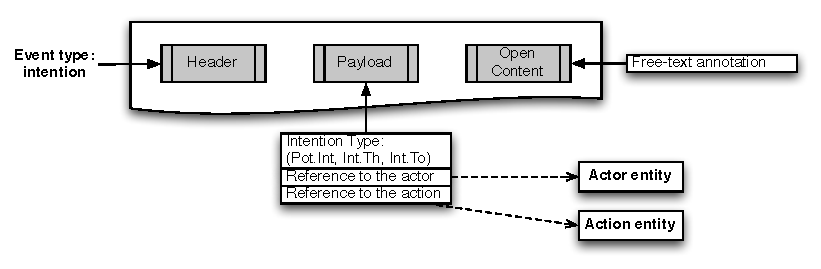
\includegraphics{intention_event.pdf} 
	\caption{Structure of an intention event}
	\label{fig:intention_event}
\end{figure}

A \emph{belief} event describes a human actor's belief in some entities or relations in a collaborative activity. For example, it can be used to indicate an actor's belief that an action has been successfully performed, or the belief that the actor has the capability to perform an action. As belief events usually refer to some changes on entities or relations in a collaborative activity, we represent each belief event by embedding an external event representing the content of the belief in its payload (Figure \ref{fig:belief_event}). However, unlike the standalone external event that indicates a change that has already happened, the change described in a belief event can be something that will happen in the future. These belief events can be used to represent the results of the human actor's projection process, i.e. what the actor expects to happen in the future. There are two attributes in a belief event's open content part: the free-text explanation of this belief, and a confidence level to describe how confident the actor is about this belief.
\begin{figure}[htbp] %  figure placement: here, top, bottom, or page
	\centering
	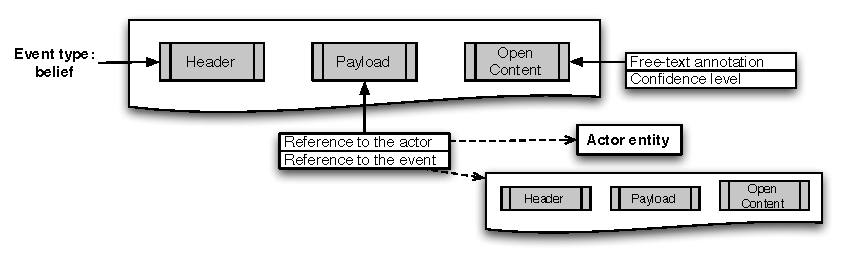
\includegraphics{belief_event.pdf} 
	\caption{Structure of a belief event}
	\label{fig:belief_event}
\end{figure}
% subsubsection internal_events (end)

\subsubsection{Composite events} % (fold)
\label{ssub:composite_events}
Composite events are a special type of events that can consist of several other events. The subsidiary events can be external or internal. Besides the list of subsidiary events, a composite event needs to also describe how these sub-events are combined together. In a simple case, a composite event can occur only when all the sub-events occur. Moreover, a composite event can occur when some of the sub-events occur, but some do not. Or it occurs when any of the sub-events occurs. A more complicated composite event language can be found in \cite{Mhl2010} that includes different relations between sub-events, such as negation, concatenation, sequence, iteration etc. To describe the composition pattern, a specific payload attribute needs to be included in a composite event's representation (Figure \ref{fig:composite_event}).
\begin{figure}[htbp] %  figure placement: here, top, bottom, or page
	\centering
	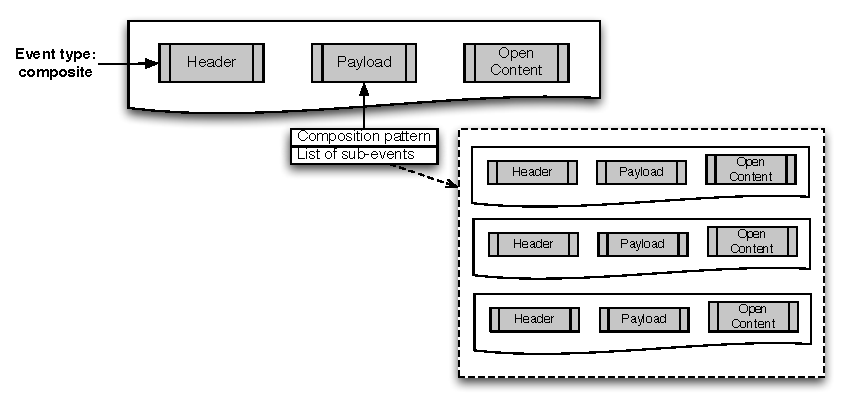
\includegraphics{composite_event.pdf} 
	\caption{Structure of a composite event}
	\label{fig:composite_event}
\end{figure}
% subsubsection composite_events (end)
% subsection event_types (end)
% section representing_events (end)

\section{The knowledge updating process} % (fold)
\label{sec:knowledge_updating_process}
The knowledge updating process describes how the aforementioned knowledge representations of collaborative activities and events are mutually developed. Each time when a new event is input into the system, it triggers the knowledge updating process. The knowledge updating process performs two important tasks: (1) it decides on how the input event influences the current collaborative activity and updates the correspondent in the PlanGraph model; (2) it augments the event representation by establishing the links between the event and the corresponding entities in the PlanGraph, and records the development of the event based on the system's reasoning.

\paragraph*{Updating knowledge about the collaborative activity} % (fold)
\label{par:updating_the_plangraph}
In general, the knowledge updating is a four-step process: \emph{association}, \emph{assessment}, \emph{elaboration}, and \emph{propagation}, through which the knowledge representation of the collaborative activity, i.e. the PlanGraph model is updated (Figure \ref{fig:updating_plangraph}).
\begin{figure}[htbp] %  figure placement: here, top, bottom, or page
	\centering
	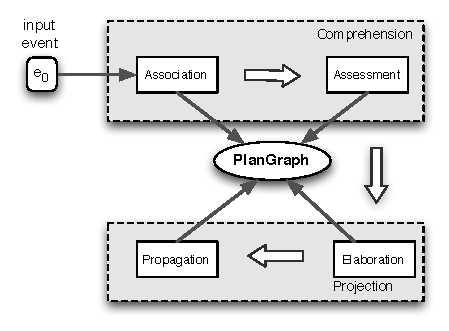
\includegraphics{updating_plangraph.pdf} 
	\caption{The knowledge updating process}
	\label{fig:updating_plangraph}
\end{figure}

\begin{enumerate}
	\item \emph{Association}. The knowledge updating starts with the association of an event with the PlanGraph model. In this step, the system searches the PlanGraph for an appropriate match between the input event and the entities and relations in the collaborative activity. If a match is found, the system uses the information stored in the event to update the corresponding entities or relations in the PlanGraph.
	\item \emph{Assessment}. The second step is to assess how the event can lead to new changes in the collaborative activity. For instance, it may trigger new actions that need to be performed, or change the current states of existing actions. 
	\item \emph{Elaboration}. Based on the assessment of the event, the elaboration step is to reason about the system's expectation on how the newly added action should be decomposed into sub-actions, or what actors will be potentially involved in these new actions. This is usually performed with domain specific knowledge, such as recipes of action performance, and role specifications of actors.
	\item \emph{Propagation}. The propagation step focuses on evaluating how the current change can be possibly propagated to other actions in the collaborative activity because of the dependencies among actions. 
\end{enumerate}

The four steps of knowledge updating process share some commonality with the human actor's awareness development processes. The \emph{association} and \emph{assessment} steps are similar to the \emph{comprehension} process, where human actors comprehend or understand the relevance of awareness information in relation to their tasks and goals. The \emph{elaboration} and \emph{propagation} can be considered as the projection of states in the near future. In this way, we can think of the knowledge updating process as the computer system's awareness development process. The only difference is that, as the human actors usually only have partial knowledge about the collaborative activity, the computer system aims to possess the knowledge of the whole collaborative activity through knowledge updating.

One thing to note is that not every event will be processed in all the four steps. Some external event may not directly link to any entities in the collaborative activity, or the system does not have the complete knowledge to assess its implications in the collaborative activity. In such case, the event may be passed directly to human actors for interpretation. The result of human actors' interpretation may generates a new internal event that starts a new round of knowledge updating, in which the system's knowledge is updated.
% paragraph updating_the_plangraph (end)

\paragraph*{Updating knowledge about the event} % (fold)
\label{par:updating_the_event_representation}
As we emphasize in the beginning, while the knowledge about the collaborative activity is updated by the new event, the event itself is also developed during the system's reasoning process. For example, in the \emph{assessment} step, an external event \emph{`TrafficBlocked'} causes the system to believe that the action to deliver a resource cannot be achieved. One one hand, this causes the system to modify the state of the delivery action in the PlanGraph. Meanwhile, the system generates a new internal event describing the system's belief about the state change of the delivery action. Later, in the \emph{propagation} step, the system may generate another internal event to indicate that because of the state change of the delivery action, the action that depends on the resource delivery will also be impacted. In this way, the original event is derived into a chain of events as the knowledge updating proceeds.

To record the development of an event in the knowledge updating process, we define an \emph{event chain} $EC$ as an ordered sequence of events: $EC=(e_0, e_1, e_2, ...)$. In the beginning of the knowledge updating process, there may be only one event $e_0$, i.e the original external event in the event chain $EC$. As the knowledge updating proceeds, more events are added to the chain. In the assessment step, the system may generate \emph{derived events} indicating the system's beliefs on how the other entities or relations in the collaborative activity have been changed due to the original event. In the propagation step, the system predicates the future state changes, and attaches more \emph{anticipatory events} to the event chain. Figure \ref{fig:knowledge_updating} shows how an event is developed into an event chain in the knowledge updating process.

\begin{figure}[htbp] %  figure placement: here, top, bottom, or page
	\centering
	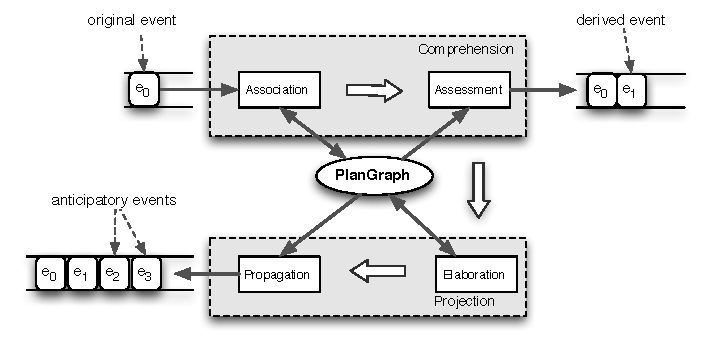
\includegraphics{knowledge_updating.pdf} 
	\caption{The development of an event chain}
	\label{fig:knowledge_updating}
\end{figure}

In order to record an \emph{event chain}, we add three additional attributes in the \emph{open content} section of every event in the chain:

\begin{enumerate}
 	\item A text string (\emph{label}) indicates the functional role of the event in the event chain, i.e. whether the event is an \emph{original} event, a \emph{derived} event, or an \emph{anticipatory} event.
 	\item An event reference (\emph{prevEvent}) points to its preceding event in the event chain. It can be optional when the current event is the \emph{original} event, but required for \emph{derived} and \emph{anticipatory} events.
 	\item An event reference (\emph{nextEvent}) points to its succeeding event in the event chain. It can be optional if the current event is at the end of the event chain.
 \end{enumerate} 

 Figure \ref{fig:event_chain_structure} shows how the additional information about the event chain is included in an event's representation. 

\begin{figure}[htbp] %  figure placement: here, top, bottom, or page
	\centering
	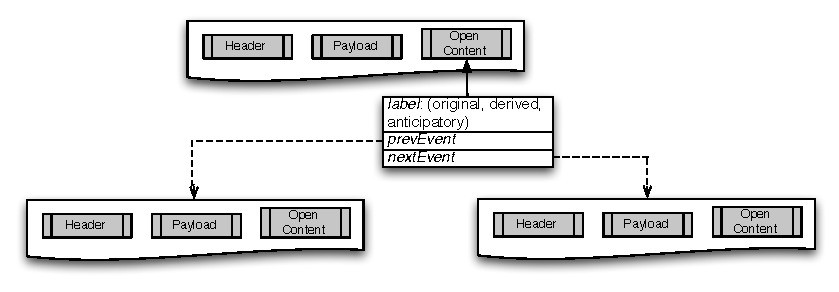
\includegraphics{event_chain_structure.pdf} 
	\caption{Event structure in an event chain}
	\label{fig:event_chain_structure}
\end{figure}
% paragraph updating_the_event_representation (end)

\subsection{Association} % (fold)
\label{sub:association}
The knowledge updating starts with establishing associations between the input event and entities and relations in the current PlanGraph model representing the collaborative activity, and uses the information carried by the event to update the PlanGraph model. Based on the different event types, the association is conducted differently.

If the event is an \emph{external event} on entities, we consider the following two cases:
\begin{enumerate}
	\item If the event indicates an existential change over time, the event is directly passed through to the assessment step, as the entity related to this event did not exist in the past.
	\item Otherwise, we search all the PlanGraph nodes to find any match with the entity described in the event based on their unique identifiers. If a match is found, we update the attribute information attached with the PlanGraph node based on the event type. If it is a state change event, we change the state of th node. If it is an existential change over space, we update the location information of the node. If it is a value comparison event, we update the corresponding attribute value. After updating the node, we add an entity reference in the event object, so that the event is direct linked to the matched PlanGraph node.
\end{enumerate}

If the event is an \emph{external event} on relations, we check for the following cases:
\begin{enumerate}
	\item If the event indicates a resource assignment relation, i.e. a resource $res_1$ is assigned to the performance of an action $act_1$. we search all the action nodes in the PlanGraph to find any match with $act_1$. If a match is found, we search for the parameters of $act_1$ in the PlanGraph to find any of them has the same resource type as $res_1$ and then assign the values of $res_1$ to the parameter. After that, we add an entity reference pointing to the parameter node in the event's payload. 
	\item If the event is related to a structural relation, e.g. an action $act_2$ is a sub-action of another action $act_1$. we search all the action nodes in the PlanGraph to find any match with $act_1$. If a match is found, we create a new node with the information described in $act_2$, and then add an entity reference pointing to this new node into the event's payload. This can be applied to other decomposition relations, such as a sub-action to achieve a condition, or a new parameter added to an existing action.
\end{enumerate}

If the event is an \emph{internal event}, we consider the following cases:
\begin{enumerate}
	\item If the event is an \emph{intention event}, we search all the action nodes in the PlanGraph to find any match with the action entity described in the event. If a match is found, we search for the \emph{Intentions} attribute associated with the action node to find whether any existing actor has the same identifier as the actor described in the event. If so, we update the intention type based on the intention event. Otherwise, we add the actor and the corresponding intention into the \emph{Intentions} associated with the action node. After that, we add an entity reference pointing to the action node in the event's payload. 
	\item If the event is a \emph{belief event} about an actor's capability to perform an action, we search all the action nodes in the PlanGraph to find any match with the action entity described in the event. If a match is found, we search for the \emph{Capabilities} associated with the action node to find whether any existing actor has the same identifier as the actor entity described in the event. If so, we update the capability type based on the belief event. Otherwise, we add the actor and the corresponding capability level into the \emph{Capabilities} associated with the action node. After that, we add an entity reference pointing to the action node in the event's payload. 
	\item If the event is other \emph{belief events}, we apply the association rules directly on the subsidiary event describing the content of the belief. 
\end{enumerate}

In sum, if an association between the event and the PlanGraph model is found, two tasks are performed. First, the corresponding PlanGraph entity or relation is updated based on the new information carried by the event. Second, the event is enriched by directly linking to the corresponding PlanGraph node, as the result of which the context of origin for this event is identified. However, not all the events can be directly associated with the PlanGraph model. Some external events may describe changes on the entities that are not currently in the PlanGraph, but implicitly impact the collaborative activity by motivating new actions or implying changes. These events will be passed to the assessment step for further analysis. 
% subsection association (end)

\subsection{Assessment} % (fold)
\label{sub:assessment}
In the assessment step, each event is evaluated to check how it can lead to new changes in the collaborative activity implicitly, where inference becomes necessary. For example, an external event indicating that a resource is now located at an actor's position implicitly indicates the successful performance of the resource delivery action to the actor. In this case, a new event showing the state change of the resource delivery action will be derived and added to the event chain along with the original event.

The knowledge stored in the PlanGraph allows the system to perform some routine assessment tasks that are universal in different application domains:
\begin{enumerate}
	\item \emph{Goal conditions on action nodes}. If an event describes changes on entities or relations that are included in an action's goal condition, the system can evaluate the action's goal condition. If the goal condition becomes holding because of this event, the system derives a new state change event on this action, and adds it into the event chain.
	\item \emph{Condition nodes}. If an event describes changes on entities or relations that are included in a condition node, the system can evaluate the condition node. If the condition becomes holding or no longer holding because of this event, it derives a new state change event on this condition, and pushes it into the event chain. 
	\item \emph{Parameter nodes}. If an event describes changes on a resource that is assigned to a parameter node, the system can evaluate the parameter's subsidiary conditions. If a  condition becomes holding or no longer holding because of this event, it derives a new state change event on this parameter, and adds it into the event chain.
\end{enumerate}

The second type of tasks that the system can perform during the assessment process is to check whether the event can activate new actions that need to be added to the collaborative activity. This type of events is usually called \emph{triggering events}, as they are often not directly associated with any existing nodes in the PlanGraph, but will trigger some new action to be added. For example, every time a new victim is found in an emergency response operation will trigger a new rescue action to be performed. In this case, the initial event about the discovery of a new victim cannot be associated with any existing actions, but asks for a new action to be performed. The assessment of action activation requires a set of pre-defined domain-specific activation rules, so that every event is searched through the activation rules to find whether it satisfies any of the conditions. If so, a new action is added to the PlanGraph, and a new derived event is generated to indicate the activation of the new action.

Furthermore, the assessment step can involve more sophisticated inference techniques, such as spatio-temporal reasoning \cite{Bennett}, pattern recognition \cite{zelnik2001event}, or case-based reasoning \cite{jakobson2004towards}, to enhance the system's reasoning capabilities. However, these reasoning techniques often require a large amount of domain knowledge to be modeled, and lack flexibility to handle unexpected events. As a result, in the assessment step, we design the system to focus on more reliable low-level routine inferences, and leave the complex, higher level assessment tasks to the human actors. Hence, some events may not be considered as contributing to the collaborative activity by the system in the assessment process. Rather, they are sent to human actors for interpretation. The result of human interpretation generates new events that are then sent back to the system to update the system's knowledge.
% subsection assessment (end)

\subsection{Elaboration} % (fold)
\label{sub:elaboration}
The main goal in the elaboration step is to advance the collaborative activity from the system's side. Based on the specification of SharedPlan theory \cite{Grosz2006}, the system can elaborate the current PlanGraph in several ways. 
\begin{enumerate}
	\item \emph{Recipe selection}. The system can contribute to the collaborative activity by retrieving a recipe for a new action from the knowledge base, i.e. by predicting the default way to perform this new action.
	\item \emph{Parameter binding}. If any of the parameters is unbound to any values, the system will search the knowledge base to find any action that can be performed to identify the value for the parameter.
	\item \emph{Condition satisfaction}. If any of the pre-conditions is not holding, the system will search the knowledge base to find any action that can be performed to satisfy the condition.
	\item \emph{Actor allocation}. If any of the actions has not been committed by any actors, the system search for the actors who might be potentially intended to or capable of performing the action. 
\end{enumerate}

The elaboration step is not performed for every event, rather it is only triggered by a subset of events that are related to the development of the collaborative activity. 
\begin{enumerate}
	\item Events on structural relations. Whenever an event indicates that a new action is a sub-action to another action, a way to identify a parameter, or to achieve a condition, the new action will be added to the PlanGraph in the association step, and needs to be elaborated.
	\item Events on goal activation. The elaboration needs to be performed whenever a new action has been added to the collaborative activity because of some triggering event in the assessment step.
	\item Events leading to condition violation. Whenever an event leads to the fact that some condition is no longer holding in the assessment step, the elaboration needs to be performed on the condition node to identify any action that can be performed to satisfy it.
\end{enumerate}

The elaboration process is achieved with the support of two types of pre-defined knowledge: (1) the recipe knowledge about how to derive an action into a sequence of parameters, pre-conditions, and subsidiary actions, how to identify a unbound parameter, or how to satisfy a condition, etc.; (2) the knowledge about actor roles and their corresponding responsibilities and capabilities. The former allows the system to elaborate the collaborative activity by adding new action, parameter, or condition nodes into the PlanGraph model; and the knowledge about role specifications allow the system to reason about who are likely to be interested in these newly added entities, or who have the capability to work on these new entities, so that the system can notify these actors about the events.

The elaboration process is predictive as it reflects the system's prediction on how the collaborative activity will be advanced due to the occurrence of the event. The system provides a default plan of performing an action, or identifies the potential actors who might be interested in it. After the elaboration process, the PlanGraph not only reflects the current state of the collaborative activity, but also shows the potential next steps based on the system's knowledge. However, the results of elaboration process never dictate how the human actors will eventually develop the action. The human actors may later generate new internal events to revise the plan generated by the system, or modify their intention or capability towards the action in the PlanGraph.
% subsection elaboration (end)
\subsection{Propagation} % (fold)
\label{sub:propagation}
Propagation is another predictive process that the system can perform to predict future state changes in the collaborative activity. It is triggered by the events that either directly indicate (in the association step) or imply (in the assessment step) state changes on the actions, and then reason about how these initial state changes can be propagated to other actions due to the multiple dependencies between them. A simple example could be: if the execution state of an action $act_1$ is changed from \emph{executing} to \emph{failed}, then the parent action $act_2$ (i.e. $SubAct(act_1, act_2)$ holds) will likely to be impacted and may also be changed to \emph{failed} if the plan is not changed. 

The propagation is performed on the dependency network, which is constructed from the PlanGraph model (Section \ref{sub:representing_dependencies}). The dependency network abstracts away the detailed information on each action node and focuses on the dependency relations among them. As a result, we can adopt more efficient network-based reasoning models to perform the propagation. In this study, we employ the Bayesian network to perform the propagation \cite{pearl1988probabilistic}. Bayesian networks are directed acyclic graphs in which the nodes represent multi-valued variables, and the arcs signify direct dependencies between the linked variables and the strength of these dependencies are quantified by conditional probabilities. The purpose of the Bayesian network is to give a belief in each possible value for each node after some evidence arrives.

In the context of our model, the nodes are the basic elements in a dependency network, i.e. dependers, dependums, and dependees, which represent the entities in the collaborative activity, i.e.  actions, resources, or conditions. The evidence fed into the network includes certain state changes on these entities. Thus, the purpose of the Bayesian network is to update the system’s belief in the states for every other node after some state change occurs on a node.

The operationalization of the Bayesian network includes three tasks: (1) the construction of the Bayesian network, (2) assignment of conditional probabilities for each link, (3) and the performance of belief updating when some events arrive.

\paragraph*{Construction of Bayesian networks} % (fold)
\label{par:construction_of_bayesian_networks}
By following the algorithm in Section \ref{sub:representing_dependencies}, we can construct the dependency network from the PlanGraph model, and then the construction of Bayesian network is very straightforward. We translate each basic element in the dependency network into a node variable, and the different dependency relations into corresponding links in the Bayesian network. The possible values for each node are determined based on the possible execution states for each type of node variables. At a given time, an action can be at one of the following states: \emph{inactive}, \emph{planning}, \emph{executing}, \emph{complete}, \emph{failing}, and \emph{delaying}. Each condition can be \emph{open}, \emph{waiting}, or \emph{holding}. Each resource can be \emph{unavailable}, \emph{waiting}, or \emph{available}. Figure \ref{fig:state_transitions} shows all the states for each type of node and the possible state transitions.
\begin{figure}[htbp] %  figure placement: here, top, bottom, or page
	\centering
	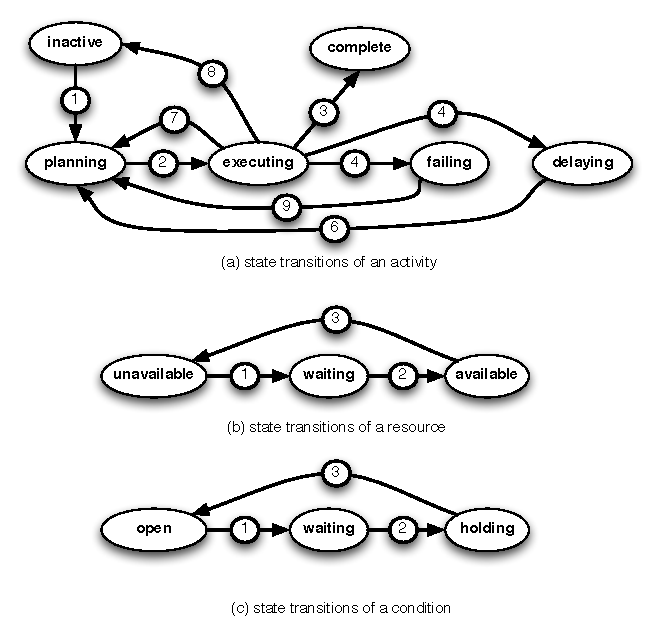
\includegraphics{state_transitions.pdf} 
	\caption{Types of node variables and possible values in a Bayesian network}
	\label{fig:state_transitions}
\end{figure}
% paragraph construction_of_bayesian_networks (end)
\paragraph*{Assignment of conditional probabilities} % (fold)
\label{par:assignment_of_conditional_probabilities}
Before any propagation commences, we need to assign the conditional probabilities for each node that form the conditional probability matrices. An element of the conditional probability matrix looks like $P(x_i|u_{1j_1}, ..., u_{nj_n})$, and gives the probability of state $i$ for node $x$ conditioned on the states of its parent nodes. For example, the conditional probability of an action node indicates the possibility of each state for this action, given the states of all the resources, conditions, actions that it depends on. 

In our study, we develop a set of heuristic rules to assign the initial conditional probabilities for each type of nodes, by evaluating the criticality of each parent node, and the opportunities for re-planning. For example, if a critical resource is needed for every possible way to perform an action, the state of the resource as \emph{failing} will definitely lead to the \emph{failing} of the action. However, if there are other possible plans to perform the action that do not require this resource, the probability of the action being failing will be decreased.

The assignment of conditional probabilities provides the system with the default reasoning capability to propagate state changes that can be later overwritten by human actors' interpretation. When a human actor changes the belief in the execution state of an action, the change will overwrite the system’s initial belief through the belief updating. Because of this interactive nature, the purpose of the initial probability assignment is just to provide a good guess about the propagation from the system's perspective and does not have to be perfectly accurate. 
% paragraph assignment_of_conditional_probabilities (end)

\paragraph*{Belief Updating} % (fold)
\label{par:belief_updating}
We follow Pearl’s belief propagation algorithm \cite{pearl1988probabilistic} to perform belief updating whenever a state change occurs. In this approach, the belief in each value of a node variable is divided into two parts: the part emerges from its ancestors and the part emerges from its descendants, and the final belief is ascribed by multiplying the two parts. As a result, the belief updating is performed as a bidirectional propagation process. 
\begin{enumerate}
	\item Starting at the node where the initial state change occurs, the system calculates how the state change will change the beliefs on each parent node. If the change on a parent node is significant, i.e. above a given threshold, the parent node becomes active, and will be further propagated to its parent. This is called \emph{causal} propagation since the updating is from a cause to an effect to indicate how a state change of the cause will lead to the change of the effect. 
	\item On the other hand, the belief updating can also calculated from an active node to their children. This is called \emph{evidential} propagation as the reasoning flows from evidence to hypothesis.
\end{enumerate}

In our approach, both the causal and evidential propagation will be performed. The causal propagation is used to provide the system's predicted state changes on the actions depending on the action associated with the initial state change. The evidential propagation occurs whenever a human actor modifies the system’s prediction on a given node and the system uses it as an evidence to trace back and revise the previous beliefs on other actions.
% paragraph belief_updating (end)

The result of the Bayesian network-based propagation will be used to enrich the event chain with anticipatory events. Starting from the node that the initial event is linked to, the system use the previous probability distribution before the propagation and the current values to perform the Cartesian product on each node. Each value in the new two-dimension table indicates the probability of each possible state change. If a significant state change has been detected (by comparing with pre-defined threshold), it will be added to the event chain as a new anticipatory event. For example, Figure \ref{fig:prob_state_change} shows the result of a propagation process on a parameter node. Before the propagation, the parameter had a high probability to be in the state of \emph{waiting}, and after the propagation, the probability distribution changed. By calculating the Cartesian product, we can find the most significant state change on the node is from \emph{waiting} to \emph{delay}, with a confidence level of $0.83808$. As a result, a new anticipatory event indicating that the state of this parameter has been changed from \emph{waiting} to \emph{delay} will be pushed into the event chain.
\begin{figure}[htbp] %  figure placement: here, top, bottom, or page
	\centering
	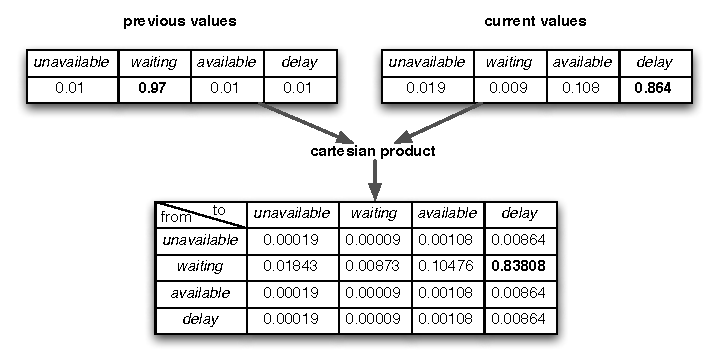
\includegraphics{prob_state_change.pdf} 
	\caption{An example of calculating state change probabilities}
	\label{fig:prob_state_change}
\end{figure}
% subsection propagation (end)
\subsection{An Example} % (fold)
\label{sub:an_example}
To demonstrate the knowledge updating process, we consider a simplified version of the victim rescue activity in the emergency response scenario to see how the PlanGraph model is updated through several consecutive events, and meanwhile the events are enriched into event chains. The task involved in this example is quite simple. Whenever a victim is found, it needs to be rescued by sending to a medical station for treatment. We assume there is only one station and one medical professional ($med$) working at it. There might be several drivers ($dr_1, dr_2, ...$) with rescue vehicles that can deliver the victim to the station.   

\paragraph*{Event 1: \emph{`NewVictim'}} % (fold)
\label{par:event_1_emph_newvictim}
The first event sent to the system is an external event reporting that a new victim has been found. The event has an event type \emph{`NewVictim'} and has several key attributes (e.g. id, occurrence time, location, required delivery time). Figure \ref{fig:update_example_event1} shows the knowledge updating process performed on this event.

\begin{enumerate}
	\item When the event is first sent to the system, the system attempts to associate it with any existing entities in the PlanGraph. Because this is the start of the activity, no association can be found. 
	\item Then the event is further processed in the assessment step, where the system checks whether the event can lead to changes on existing actions or trigger new action. By checking the association rules stored in the knowledge base, the system finds that every \emph{`NewVictim'} event will activate the goal to rescue the victim. Following this activation rule, the initial PlanGraph is generated with just one action node (\emph{`rescue'}) representing this new action to rescue the victim.
	\item After the assessment, the system finds that a new action has been added to the PlanGraph, which triggers the elaboration process. The system searches the knowledge base to find a recipe for the \emph{`rescue'} action, and extends the PlanGraph model with the parameters, conditions, and sub-actions. In this example, there is one parameter that is the \emph{`victim'} who needs to be rescued, one condition (\emph{`victimAtStation'}) that is the victim needs to be located at the medication station, and then the sub-action (\emph{`medicalTreat'}) to perform the medical treatment on the victim. As these subsidiary entities are also new to the PlanGraph, the elaboration continues on each of them. During the elaboration of the parameter, the system assigns it with the value from the input event. The condition is elaborated with a new action (\emph{`transport'}) to achieve it, which is further elaborated into subsidiary parameters and actions (\emph{`vehicle'}, \emph{`pickup'}, \emph{`deliver'}). During the elaboration of action \emph{`medicalTreat'} and action \emph{`transport'}, the system also looks for the potential actors who might be interested in these actions. Based on the actor $med$'s role as a medical professional, the system believes that $med$ has the potential intention ($pot.int$) and is able ($able$) to perform the \emph{`medicalTreat'} action. Similarly, the system believes all the drivers $dr_1, dr_2, ...$ have the potential intention ($pot.int$) and are able ($able$) to perform the \emph{`transport'} action.
	\item Because the event does not indicate any state change on current actions, the propagation is skipped.
\end{enumerate}

As we can see in Figure \ref{fig:update_example_event1}, after the knowledge updating process, the PlanGraph is updated to reflect the system's prediction on how the activity will be advanced. At the same time, the initial event is augmented with a new attribute pointing directly to the parameter node \emph{`victim'} in the PlanGraph.
\begin{figure}[htbp] %  figure placement: here, top, bottom, or page
	\centering
	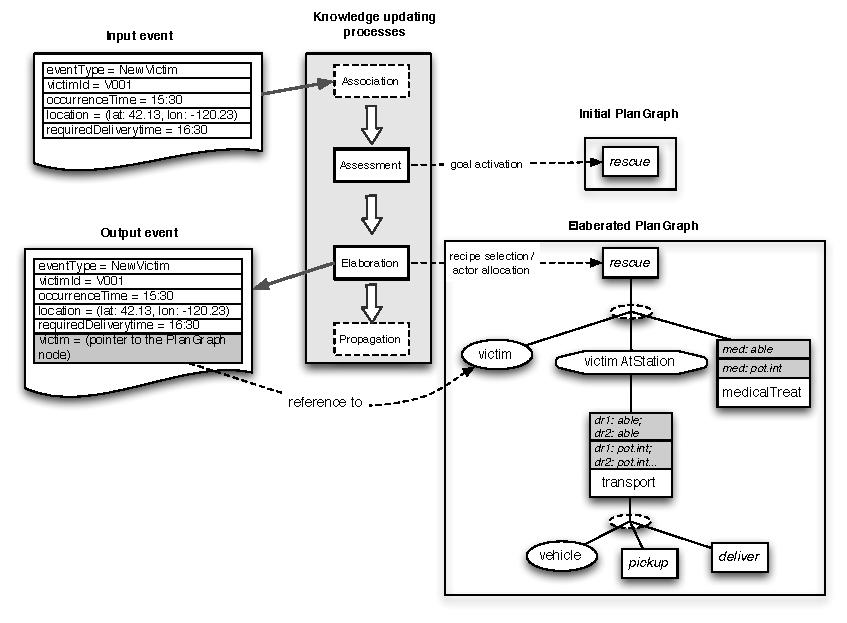
\includegraphics{update_example_event1.pdf} 
	\caption{The knowledge updating example (\emph{Event 1})}
	\label{fig:update_example_event1}
\end{figure}
% paragraph event_1_emph_newvictim (end)
\paragraph*{Event 2: \emph{`IntentionChange'}} % (fold)
\label{par:event_2_emph}
The second event is an internal event that is generated by the driver $dr_1$. After interpreting the first \emph{`NewVictim'} event, $dr_1$ intends to perform the \emph{`transport'} action to deliver this new victim to the medical station. As a result, he generates this \emph{`Intention'} event to update his intention on the \emph{`transport'} action from $pot.int$ to $int.to$. This \emph{`IntentionChange'} event has several key attributes, including the actor's id ($dr_1$), the action $dr_1$ intends to perform (\emph{`transport'}), and the intention type ($int.to$).

As the system receives this event, it first attempts to associate the event with any existing entities in the PlanGraph model. Because this is an intention event, the system traverses through the PlanGraph to search for any match between the action (\emph{`transport'}) mentioned in the event and the action nodes in the PlanGraph. As the system is able to find such a match, the system uses the information in the event to update $dr_1$'s intention level on action \emph{`transport'}. Meanwhile, the corresponding attributes of the actor and the action in the event are updated with reference to the corresponding nodes in the PlanGraph.

The knowledge updating process then proceeds to the following steps, but none of them leads to further changes in both the PlanGraph and the event itself. Figure \ref{fig:update_example_event2} shows the whole process performed on the second event.
\begin{figure}[htbp] %  figure placement: here, top, bottom, or page
	\centering
	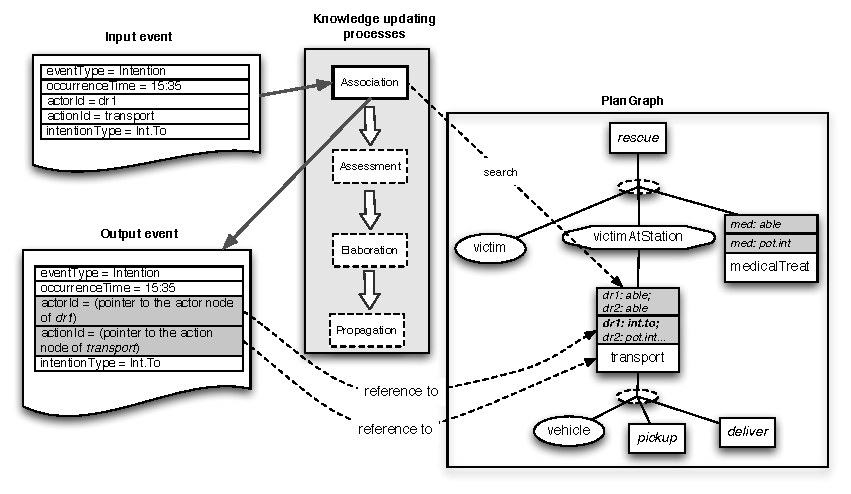
\includegraphics{update_example_event2.pdf} 
	\caption{The knowledge updating example (\emph{Event 2})}
	\label{fig:update_example_event2}
\end{figure}
% paragraph event_2_emph (end)

\paragraph*{Event 3: \emph{`FuelLevelLow'}} % (fold)
\label{par:event_3_}
The third event happens after $dr_1$ starts the action \emph{`transport'} and is on the way to pick up the victim. It is an external event indicating that the fuel level on driver $dr_1$'s vehicle is running extremely low. The event has an event type \emph{`FuelLevelLow'} and carries information about the driver, the vehicle, and the current fuel level. Figure \ref{fig:update_example_event3} shows the knowledge updating process performed on this event.

\begin{enumerate}
	\item When the event is first sent to the system, the system attempts to associate it with any existing entities in the PlanGraph model. Because this is an external event indicating an attribute change on an entity, the system traverses through the PlanGraph to search for any match between the entity (\emph{`vehicle'}) mentioned in the event and the nodes in the PlanGraph. When the system is able to find such a match, the system uses the information in the event to update the value attached to the parameter (\emph{`vehicle'}).
	\item Then the event is further processed in the assessment step, where the system checks whether the event can lead to changes towards the action performance. By checking the conditions attached with the parameter (\emph{`vehicle'}), the system finds that because of the low fuel level on the vehicle, the parameter becomes unavailable to perform the \emph{`transport'} action. As a result, a new state change event \emph{`ExecStateChange'} is derived to describe the execution state of the parameter, and is added to the output event chain.
	\item As no new action nodes are added to the PlanGraph, the elaboration process is skipped.
	\item Because a state change event has been derived in the assessment step, the system attempts to predict future state changes in the propagation step. A Bayesian network is constructed based on the current PlanGraph model and used to reason how likely the other entities in the PlanGraph will be impacted by the initial state change. After the Bayesian network-based reasoning, the system finds that $dr_1$'s action to pick up the victim (\emph{`pickup'}) is likely to change its state from \emph{executing} to \emph{delaying}, and a new anticipatory event describing this state change on the execution state of the \emph{`pickup'} action is generated, and added to the output event chain.
\end{enumerate}

As we can see in Figure \ref{fig:update_example_event3}, after the knowledge updating process, the initial event is augmented into an event chain with three events: the original external event \emph{`FuelLevelLow'}, the state change event on the parameter \emph{`vehicle'} derived in the assessment step, and the anticipatory event predicting the state change on the action \emph{`pickup'} in the propagation step. This example shows the idea that not only the knowledge representation of the collaborative activity, i.e. PlanGraph model is modified during the knowledge updating process, but also the original event is enriched with system generated knowledge.

\begin{figure}[htbp] %  figure placement: here, top, bottom, or page
	\centering
	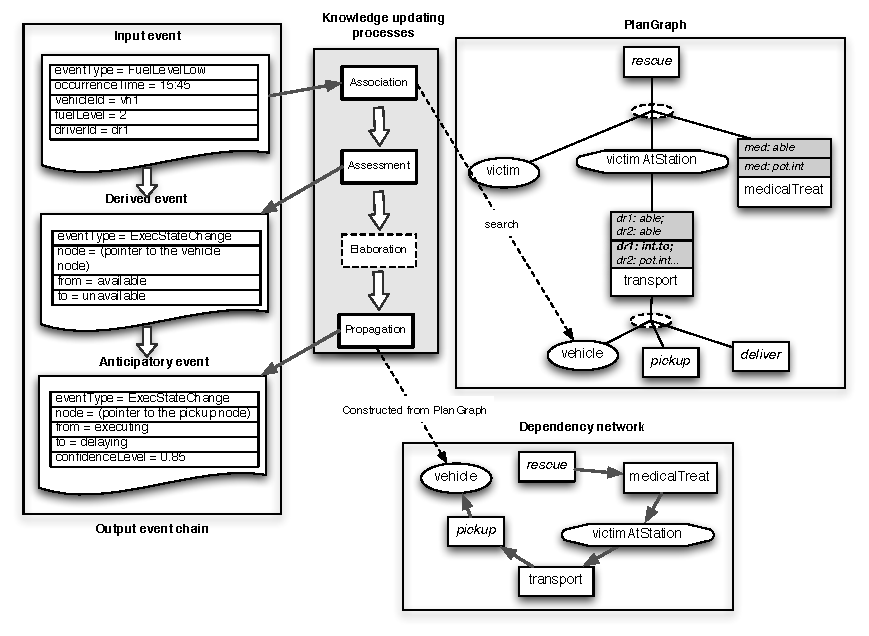
\includegraphics{update_example_event3.pdf} 
	\caption{The knowledge updating example (\emph{Event 3})}
	\label{fig:update_example_event3}
\end{figure}
% paragraph event_3_ (end)
% subsection an_example (end)
% section knowledge_updating_process (end)

\section{Discussion} % (fold)
\label{sec:knowledge_representation_discussion}
In this chapter, we first focus on the knowledge representation of collaborative activities. We employ the PlanGraph model to represent the entities and relations in collaborative activities, and then use this model to derive knowledge about local scopes of work and dependencies. The PlanGraph model exhibits some important characteristics that make it suitable to satisfy the three requirements for representing collaborative activities described in Section \ref{sub:computational_representation_of_the_field_of_work}.

\begin{enumerate}
   \item The PlanGraph model represents collaborative activities as hierarchically structured actions. The components of actions, parameters, conditions can be used to capture all the entities and the relations between them. With the knowledge represented in the PlanGraph, the local scopes and dependencies can also be easily identified. 
   \item A critical point made in the PlanGraph model is the emphasis on the development of collaborative activities. With the development of the activity, the PlanGraph model needs to be updated accordingly, so that it always  reflects the current state of the changing activities.
   \item Based on the formalization in SharedPlan theory, the PlanGraph model can be computationally implemented, and it provides a set of reasoning capabilities that can be operationalized to support computer reasoning.  
\end{enumerate}

Following that, we discuss the representation of events and identify the major event types supported in this study. The central idea of our approach is the interaction between these two knowledge components, which has been described in the knowledge updating process. On one hand, the various events are consumed by the computer system to update its PlanGraph-based representation of collaborative activities. On the other hand, the PlanGraph model enriches the events with more meaningful contextual information, which is used in next chapter to support event-driven awareness processes. 
% section knowledge_representation_discussion (end)
% chapter knowledge_reprsentation_and_updating (end)




 


%!TEX root = ../BoYu-Dissertation.tex
\graphicspath{{Figures/}}

\chapter{Our Approach: Updating Knowledge Representation} % (fold)
\label{cha:knowledge_updating}

\section{Construction and Development of the Model} % (fold)
\label{sec:construction_and_development_of_the_model}
different ways to do it:

1. the development of algorithms and heuristics for inferring mental state on the basis of observed actions While these algorithms and heuristics are domain independent, they require much rich domain-specific knowledge to work.

2. Human complementary work has attempted to avoid the problem of intent recognition by developing domain- specific languages and interfaces that allow users to specify their goals and plans directly.


these capabilities can be added incrementally to the basic approach to ensure a favorable ratio of cost (of knowledge engineering and runtime computation) to benefit (enhanced user performance). In addition, both more and less complicated versions of these capabilities exist and can be applied. For example, goal recognition can be done the hard way, i.e. using AI plan recognition techniques. However, a very simple technique is to hard-wire in one or more domain goals. As discussed above, a third approach (of intermediate complexity) is to represent domain goals and plans in the interface and allow users to specify them explicitly. Fischer and colleagues 85.s6 discuss how combining a goal specifica- tion component with a critiquing system improves the quality of system advice t


Information about users may be acquired explicitly, by engaging a user in an interaction expressly designed to acquire information, or implicitly, inferring information on the basis of user actions 58. Both methods have draw- backs. If users must answer system questions or fill out a form, they may find this obtrusive and may have a difficult time characterizing themselves accurately. On the other hand, implicit acquisition can be a difficult computational task, depending on the type of user model being constructed. Plan recognition, as previ- ously mentioned, is a very difficult computational problem. Among other things, it is difficult to know when a user is starting a new plan (as opposed to continuing the current one), users may suspend and resume plans, actions may be part of more than one plan, and there may be multiple plans for a single goaP 6. Stereotypes can be easier to recognize; each stereotype generally has a triggering condition that, when satisfied, leads the system to categorize the user as a member of that stereotype. Also, some representations of user pref- erences are fairly simple, and thus can be computed easily. For example, simple statistics on what messages a user reads in Net News may allow a system to filter the messages the user sees in the future 7°.


However, ITS researchers have been active in designing interaction techniques that allow users to express their intent directly, rather than requiring the system to guess it 72-74.. By analyzing how a class of users works within a particular task domain, say symbolic integration, financial analysis, or medical diagnosis, researchers develop a set of goals and plans for achieving these goals. These goals and plans are represented formally in a knowledge representation language and also represented graphically as objects in a direct manipulation interface 43. Users then directly specify their goals and plans. This benefits both user and system. The user is given a medium for making problem solving explicit, rather than having to do it mentally or using noncomputational aids such as paper and pencil. The system gains access to a high-level specification of what it is that the user is trying to accomplish, thus simplifying the computations required to play a useful role in the interaction. For example, computations to track and display finished and unfinished steps in the plan, to fill in low-level details required in executing a plan, and to determine whether a plan is inappropriate are very useful and much simpler than plan recognition. Checklists 75,76, computerized versions of the everyday to- do list, are a specific interaction resource used for orga- nizing interaction and tracking and displaying progress toward a goal.

Systems by Self for logic tutoring 73 and Singley for
algebra rate of change problems 77 explored the use of `goal posting'. For example, in Singley's system, a user selects a goal such as `find dp/dt in terms of t'. She next chooses a plan operator for achieving the goal, such as using the chain rule. Several subgoals might have to be satisfied before the operator can be applied. At all times, the system keeps track of which goals have and have not been satisfied, visually differentiating the current goal, satisfied goals, and unsatisfied goals. Empirical studies showed that the goal posting tech- nique improved user performance and facilitated learn- ing.

In addition to techniques for directly specifying goals,
another important notion is the incremental specifica- tion of goals. People typically do not form precise defi- nitions of goals to accomplish, then plan to achieve their goals, and then carry out their plans. Rather, acting, planning, and forming and pursuing goals are interleaved. A number of interaction techniques have been explored that support incremental specification of goals in exploratory activity. The retrieval by reformula- tion 8~82 information retrieval technique interleaves query definition, querying, and evaluation of results. Experiments with critics (discussed in detail in the next section) have shown that users may refine their goals on the basis of the delivery of advice from a system about user actions. They begin by specifying information they know and care about, and then gradually refine and elaborate it in response to system advice


\subsection{The Development of PlanGraph} % (fold)
\label{sub:the_development_of_plangraph}





Considering the collaborative activity as a process from a partial SharedPlan to a full SharedPlan among the participants, the PlanGraph, which is used to represent the collaborative activity, should also be considered as dynamically developed. To facilitate the development of PlanGraph, the PlanGraph model provides the reasoning mechanisms to decide how the interaction between the system and human participants, or between the human participants, influences the state of collaborative activity and update the changes in the PlanGraph. In general, the reasoning mechanism in PlanGraph model includes two steps: the plan explanation and the plan elaboration.

\subsubsection*{Plan Explanation}
Participants in a collaborative activity need to interact with each other to contribute to the activity. It is through the communication between the participants that collaboration can be enacted. Therefore, the input of an agent can be treated as the way that the agent tries to express their intentions to the other agents in the collaborative activity. Plan explanation is the step where the system attempts to explain how the meanings of the new piece of interaction relate to the current PlanGraph. In general, the new input is said to be meaningfully merged with the current collaboration context if one of the following conditions is satisfied:

\begin{enumerate}
\item The new input provides a piece of information that helps the agents to assign/change a value to a parameter in the current PlanGraph. 
\item The new input provides more details on the performance of a complex action in the PlanGraph. For example, the user suggests performing a sub-action or identifying a parameter in order to complete the action.
\item The new input helps to establishing necessary mental states for a collaborative action. In this case, the agent's new input serves as an indicator of the speaker's mental attitudes, such as confirmation or refusal towards certain states of fairs. 
\end{enumerate}

If the new user input can be successfully explained in current PlanGraph, it will be merged to update the PlanGraph accordingly, i.e. the contextual information about the ongoing activity is changed.

\subsubsection*{Plan Elaboration}
The main goal in elaboration stage is to advance the collaborative activity from the system side based on the change from the new input. After the interpretation process, the context of the activity is changed. Therefore, the system needs to elaborate the PlanGraph to accommodate the changes. The elaboration process begins with the root node of the PlanGraph and uses the depth-first traverse to visit the whole plan based on reasoning rules associated with PlanGraph model. The elaboration ends when no more parts of the PlanGraph can be further elaborated.

The system can elaborate the PlanGraph in several ways. First, the system can contribute to the collaborative activity by retrieving a recipe for an action from the knowledge base. Second, the system can execute the basic actions that can be performed without further inputs from other human agents. Lastly, the system can identify the value for a parameter by retrieving the default or suggested values from the knowledge base. 

After the elaboration process, the PlanGraph again reflects the current state of the collaborative activity. Therefore, the information from the PlanGraph can be used by the system to represent the current state of the activity context. 

This elaboration process also attempts to discover all the open nodes in the PlanGraph that might be addressed later in the collaboration, such as unidentified parameters, unperformed actions, conflicting beliefs, missing details, or ambiguous choices. These possible open nodes are   stored in an agenda to include all the possible attentional states that require further development in the collaboration. During the elaboration process, when the system encounters some problem to elaborate an action node, is unable to identify the value of a parameter, or fail to execute an action, the system will put the node into the agenda.
% subsection the_development_of_plangraph (end) 

% section construction_and_development_of_the_model (end)

% chapter knowledge_updating (end)




 


%!TEX root = ../BoYu-Dissertation.tex
\graphicspath{{Figures/}}

\chapter{Architecture and Implementation} % (fold)
\label{cha:system_implementation}
To validate our computational approach, a prototype system EDAP (Event-driven awareness promotion) is implemented in this study. EDAP server provides a generic event-driven infrastructure for awareness promotion that can be applied in different application domain. EDAP client is a standalone Web-based interactive awareness system that is used to demonstrate the functionality of our approach. In this chapter, we first describe the architecture of the system. Then we describe the implementation details of the server and client.

\section{Architecture of EDAP} % (fold)
\label{sec:architecture_of_edap}
EDAP follows a typical client/server architecture model (Figure \ref{fig:edap_architecture}). The EDAP server provides the major functions of the event-driven awareness promotion, i.e. it maintains the knowledge representation, performs the knowledge updating and event processing. The EDAP client provides the visual and interactive environment that allows the user to perceive and interpret events,  generate new events, and manage subscriptions and visibility policies.

\begin{figure}[htbp] %  figure placement: here, top, bottom, or page
	\centering
	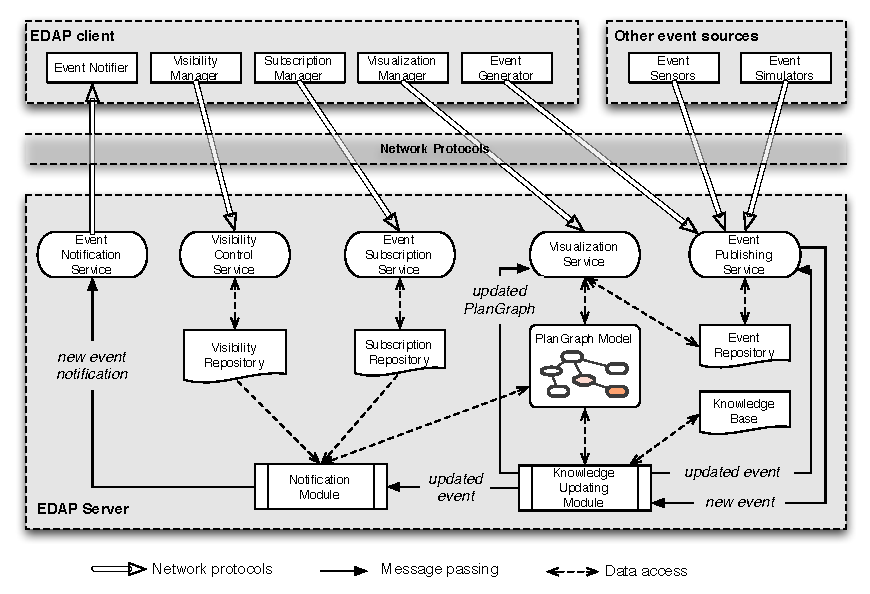
\includegraphics{edap_architecture.pdf} 
	\caption{Architecture of EDAP}
	\label{fig:edap_architecture}
\end{figure}

The interaction between the client and server follows the service-oriented network protocols. The REST protocol is used to implement the request/response communication style, i.e. clients initiate requests to servers and servers process requests and return appropriate responses. The COMET protocol is used to offer the push notification from the server to the client by maintaining a long-held HTTP request between them. 

The EDAP client provides several components that can interact with the server. The \emph{Event Generator} is used to create new events in the externalization process, and post the new events to the server for processing. The \emph{Visualization Manager} requests visualization specifications about the event view, activity view, and context view from the server, and render them in the client's interface. The \emph{Subscription Manager} requests the existing subscriptions from the server, provides the interface for the user to manage them or create new ones, and then send the modifications back to the server. The \emph{Visibility Manager} provides the similar function as the \emph{Subscription Manager} to manage visibility policies. The \emph{Event Notifier} establishes a long-polling connection with the server. Whenever a new event notification is sent from the server, it applies the corresponding notification style to notify the user. 

To respond to client requests, the EDAP server provides several components in the form of web services to handle the different types of requests. The \emph{Event Publishing Service} responds to the new events posted from the client or other event sources, stores them in the event repository, and notifies the \emph{Knowledge Updating Module} to process them. The \emph{Visualization Service} generates the visualization specifications for the event view and activity view based on the knowledge from PlanGraph model and event repository. The \emph{Event Subscription Service} responds to the \emph{Subscription Manager} and updates the subscription repository. The \emph{Visibility Control Service} responds to the \emph{Visibility Manager} and updates the visibility policy repository. The \emph{Event Notification Service} responds to the message passed from the \emph{Notification Module} whenever a new event notification is generated, and push it to the corresponding clients. Besides these service-oriented modules, the server also includes two important processing modules: the \emph{Knowledge Updating Module} perform the knowledge updating as described in Section \ref{sec:knowledge_updating_process} whenever new events are received; and the \emph{Notification Module} provides the local scope-based event notification mechanism (Section \ref{sec:event_notification_mechanism}) to distribute events. 

The communication between modules in the EDAP server is achieved through a limited form of the publish/subscribe interaction. Each module can publish important messages during its performance, and the other modules who need to respond to these messages need to subscribe to them. In this way, the interaction between modules can be asynchronous so that they do not block each other while waiting for others to finish their task. In addition, it provides a distributed interaction style that allows the different modules to be deployed across multiple machines. 
% section architecture_of_edap (end)

\section{Implementation of EDAP Server} % (fold)
\label{sec:implementation_of_edap_server}
The functional modules EDAP server is implemented using the Python programing language, and the web services are developed in the Django framework. The three data repositories, i.e. event, subscription and visibility repositories, as well as the knowledge base, are implemented as PostgreSQl databases. In the following, we describe the implementation details on major modules and the repositories are discussed within the respective modules that can manipulate them. 

\subsection{Service-oriented modules} % (fold)
\label{sub:service_oriented_modules}
The EDAP server includes five service-oriented modules to handle the different types of client requests. 

\paragraph*{Event Publishing Service} % (fold)
\label{par:event_publishing_service}
The \emph{Event Publishing Service} is the first responder to the new events that are published to the system, and its major responsibility is to store the events in the event repository. There are two types of event sources where the \emph{Event Publishing Service} can receive events:

\begin{enumerate}
	\item Events can come externally from the different types of clients as HTTP requests, including the EDAP client or other event sensors or simulators. For these events, after storing them in the repository, the service also needs to send out a \emph{`NewEvent'} message notifying the \emph{Knowledge Updating Module} to perform knowledge updating on the new event.
	\item They can also come from the \emph{Knowledge Updating Module} as it generates new derived or anticipatory events. These events are published by the \emph{Knowledge Updating Module} as \emph{`UpdatedEvent'} messages, and the \emph{Event Publishing Service} needs to subscribe to them and store them in the repository. 
\end{enumerate}

The events received by the \emph{Event Publishing Service} are described as attribute-value tuples, and the service needs to store these events in the event repository. The event repository needs to be semi-structured as the different event types supported by the system can have different set of attributes. However, this cannot be directly achieved in a relational database like PostgreSQl. As a result, we only store the header of each event directly in the data tables, but add two additional long text field (\emph{payload} and \emph{opencontent}) for each record. These two fields store the XML formatted tuples corresponding to the attributes in the event's payload and open content. Besides the event table that stores all the events, the event repository also includes a relation table to record the event chains or event propagation trees. Whenever an event is added to the repository, a new record is added to the event development table as well with the id of parent event (null for original events) and the current event, along with the label indicating the type of the event. Figure \ref{fig:event_repository} shows the data tables in the event repository. 

\begin{figure}[htbp] %  figure placement: here, top, bottom, or page
	\centering
	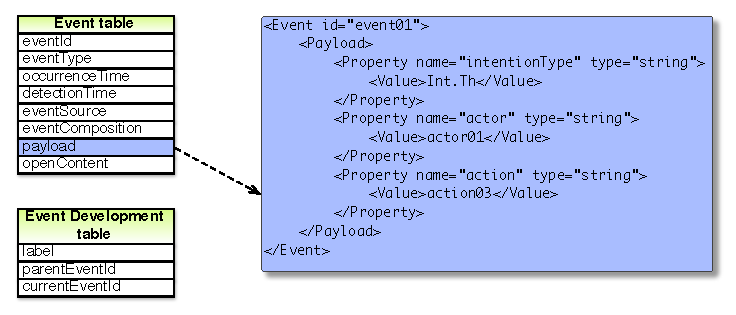
\includegraphics{event_repository.pdf} 
	\caption{Data tables in the event repository}
	\label{fig:event_repository}
\end{figure}
% paragraph event_publishing_service (end)

\paragraph*{Visualization Service} % (fold)
\label{par:visualization_service}
The \emph{Visualization Service} responds to the client's request for visualizing the event view or activity view. The service retrieves the necessary data from event repository or PlanGraph model, uses it to generate a visualization specification in the JSON format and sends it back to the client. 

For the request to visualize the event view given the current event under interpretation, the service searches the event repository recursively to find all the events that are included in the event propagation tree, and generates a JSON object to represent the tree structure.

In order to generate the visualization specification for the activity view, the service maintains the most recent version of the local scopes and dependency network constructed from the PlanGraph model. The \emph{Visualization Service} subscribes to the message \emph{`updatedPlanGraph'} that is published by the \emph{Knowledge Updating Module} each time the PlanGraph model is changed. Hence, whenever the \emph{Visualization Service} receives such message, it uses the PlanGraph model to reconstruct the local scopes and dependency network so that it always keeps the newest version. Whenever the client requests an activity view given a specific user, the user's local scope is first retrieved, and the entities in the local scope are added to the visualization specification. Then the entities in the local scope are searched in the dependency network recursively to find all the other entities that have dependency relations with them, and these entities outside the local scope are added to visualization specification.
% paragraph visualization_service (end)

\paragraph*{Event Subscription Service} % (fold)
\label{par:event_subscription_service}
The \emph{Event Subscription Service} responds to the client's request to list all the current subscriptions, add a new subscription, modify or delete an existing subscription. The existing subscription of each user is stored in the subscription repository. If the request is to add a new subscription, a new record will be added into the repository. If the request is to modify or delete an existing one, the subscription id will be used to identify the record in the repository and perform the update or delete operation. 

Because the event pattern in each subscription is semi-structured with multiple filter expressions, we also use the XML formatted text field to store the filters for each subscription. Figure \ref{fig:sub_repository} shows the subscription table with an example of the XML formatted event pattern that include all the three types of filter expressions discussed in Section \ref{sub:managing_subscriptions}.

\begin{figure}[htbp] %  figure placement: here, top, bottom, or page
	\centering
	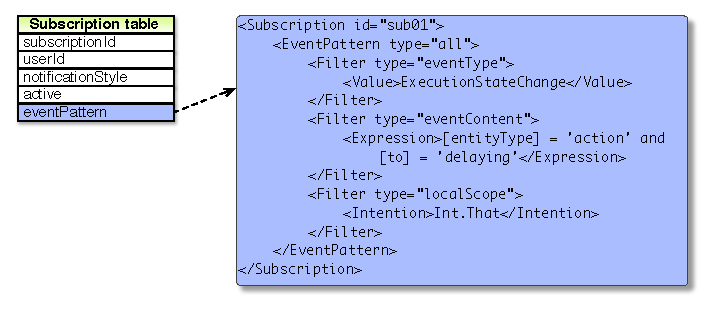
\includegraphics{sub_repository.pdf} 
	\caption{An example subscription record}
	\label{fig:sub_repository}
\end{figure}
% paragraph event_subscription_service (end)

\paragraph*{Visibility Control Service} % (fold)
\label{par:visibility_control_service}
The \emph{Visibility Control Service} works in the similar way as the \emph{Event Subscription Service}, to manipulate the visibility repository to retrieve, add, modify or delete visibility policies. Unlike the subscriptions, each visibility policy has three semi-structured fields: the \emph{eventPattern} is similar to the event pattern in subscriptions, the \emph{receiverPattern} includes the filter expressions that are used to define the receivers to whom the event is visible, and \emph{attributeList} is the list of visible attributes. Figure \ref{fig:vis_repository} shows an example of a record in the visibility repository.
\begin{figure}[htbp] %  figure placement: here, top, bottom, or page
	\centering
	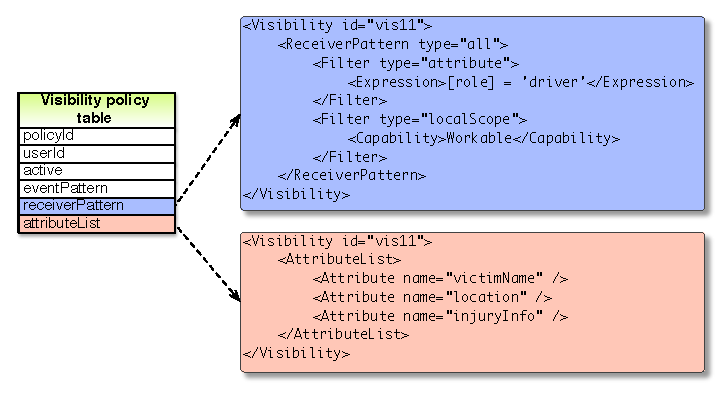
\includegraphics{vis_repository.pdf} 
	\caption{An example visibility policy record}
	\label{fig:vis_repository}
\end{figure}
% paragraph visibility_control_service (end)

\paragraph*{Event Notification Service} % (fold)
\label{par:event_notification_service}
The \emph{Event Notification Service} maintains a long polling connection with each client so that it can push new event notifications to the client. The service stores a routing table that maps each user id to the corresponding client connection. The service subscribes to the message \emph{`newEventNotification'} that is published by the \emph{Notification Module} each time a new event notification is generated. Whenever the \emph{Event Notification Service} receives such a message, it searches the routing table to find a match between the receiver of the notification and the client connection. If a connection is found, the service pushes the event notification to the corresponding user via the client connection. 
% paragraph event_notification_service (end)
% subsection service_oriented_modules (end)

\subsection{The Knowledge updating module} % (fold)
\label{sub:the_knowledge_updating_module}
The \emph{Knowledge Updating Module} performs the knowledge updating process as we described in Section \ref{sec:knowledge_updating_process}. As the \emph{Knowledge Updating Module} manipulates the PlanGraph model, we first describe how the PlanGraph model is implemented, then discuss the implementation of the knowledge updating process.

\paragraph*{Implementation of the PlanGraph} % (fold)
\label{par:implementation_of_the_plangraph}
The PlanGraph is implemented in the object-oriented paradigm as a dynamic data structure by several data objects. The overall \emph{PlanGraph} object points to the root plan node. Each \emph{PlanNode} objects includes attributes recording the parent node and the subsidiary plan nodes, which together allows the recursive traverse throughout the PlanGraph hierarchy. 

The \emph{PlanNode} has three types of subsidiary classes, corresponding to the three types of nodes in the PlanGraph model.

\begin{enumerate}
	\item Each \emph{ActionNode} defines the properties of an action, such as the type of the action, whether it is a basic or complex action, the execution state, the current recipe of the action. Each \emph{ActionNode} also includes two slots to store the actors' intentions and capabilities towards the action. Besides, each \emph{ActionNode} includes a list of parameters and the conditions.
	\item Each \emph{ParamNode} object represents a parameter that includes the type of the parameter, the execution state, the values, and the list of conditions about the parameter.
	\item Each \emph{CondNode} object represents a condition that includes the type of the parameter, the execution state, and an expression indicating the content of the condition.
\end{enumerate}
\begin{figure}[htbp] %  figure placement: here, top, bottom, or page
	\centering
	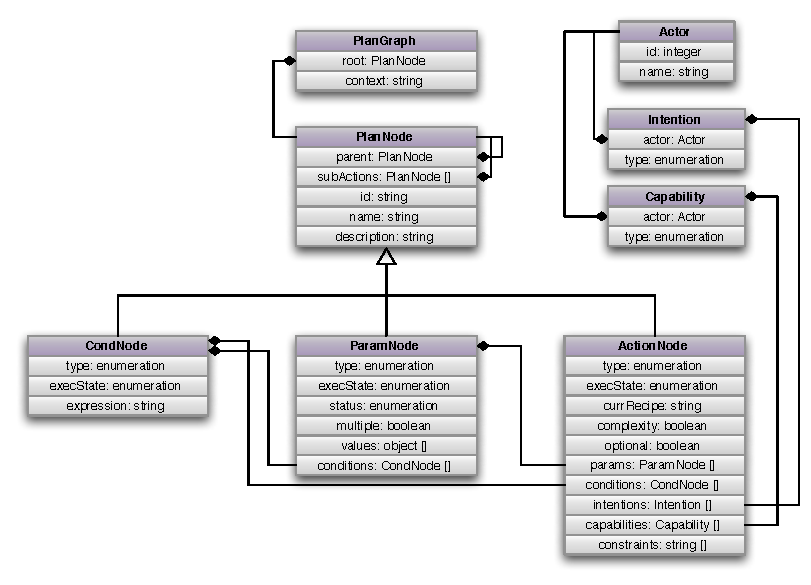
\includegraphics{pg_class_diagram.pdf} 
	\caption{The class diagram of the PlanGraph}
	\label{fig:pg_class_diagram}
\end{figure}
% paragraph implementation_of_the_plangraph (end)

\paragraph*{Implementation of the knowledge updating process} % (fold)
\label{par:implementation_of_the_knowledge_updating_process}
The \emph{Knowledge Updating Module} includes four subsidiary modules, complying with the four steps of the knowledge updating process. 

\begin{enumerate}
	\item \emph{Association} sub-module establishes the association between the input event and the current PlanGraph mode by searching all the nodes in the PlanGraph. It starts with the recognition of event type for each input event, as the different event types are treated differently. The association is implemented as a native function in Python that follows the search strategies we discussed in Section \ref{sub:association}. Once an association is found, it updates the value of the corresponding node in the PlanGraph, and then add the pointer to the node into the event object.
	\item \emph{Assessment} sub-module evaluates each event check how it can lead to changes towards the action performance, such as the execution state change of an action, or a condition. This sub-module is achieved by defining a set of assessment rules and employing a knowledge engine Pyke to enable the forward chaining inference. The knowledge engine uses the PlanGraph to assess all the possible changes due to the new information stored in the event, and then generate new events to represent these changes. Whenever a new event is generated in this step, the module publishes a new \emph{`NewEvent'} message, so that the other modules who subscribe to it can get notified.
	\item \emph{Elaboration} sub-module advances the collaborative activity from the system side based on the change from the new event. The elaboration is achieved with the support of two types of knowledge stored in the knowledge base: (1) the recipe knowledge about how to derive an action into a sequence of parameters, pre-conditions, and subsidiary actions, how to identify a unbound parameter, or how to satisfy a condition, etc.; (2) the knowledge about actor roles and the potential intentions and capabilities towards actions. These two types of knowledge are stored in the \emph{knowledge base} in the form of a PostgreSQl database. The content of each recipe is stored in an XML formatted text field along with other general information about the recipe. The actor role specifications are stored in a data table mapping each role to the potential intended action type, or the actions that the actors in the role are capable of performing.
	\fxwarning{add an example recipe here.}
	\item \emph{Propagation} sub-module is a standard Bayesian network-based reasoning process. This module first constructs the dependency network from the PlanGraph model following the algorithm described in Section \ref{sub:representing_dependencies}. Then we employ the open source Python library, OpenBayes, to propagate the state change in the dependency network. Based on the results of the propagation, we generate new events to represent these changes, and new \emph{`NewEvent'} messages will be published to notify other modules.
\end{enumerate}

After the four steps have been performed, the knowledge updating module publishes two new messages \emph{`UpdatedEvent'} and \emph{`UpdatedPlanGraph'}. The former is used by the \emph{Notification Module} to start generating event notifications, and the latter notifies the \emph{Visualization Service} to reconstruct the local scopes and dependency network.
% paragraph implementation_of_the_knowledge_updating_process (end)
% subsection the_knowledge_updating_module (end)

\subsection{The Notification module} % (fold)
\label{sub:the_notification_module}
The \emph{Notification Module} performs the event notification algorithms to generate event notifications after the knowledge updating process is done on each event, i.e. whenever it receives a new message \emph{`UpdatedEvent'} from the \emph{Knowledge Updating Module}. The \emph{Notification Module} generates event notifications in three steps, and different type of knowledge is used in each step.

\begin{enumerate}
	\item The PlanGraph is used in the first step to perform the local scope-based filtering as described in Section \ref{sub:event_filtering_algorithm}. The module implements the $FILTER\textrm{-}LS$ algorithm as a standard Python function and execute it on each user participated in the PlanGraph. If the function returns true, the second step is performed.
	\item During the second step, the user's subscriptions are retrieved from the subscription repository, and the event is evaluated against each of the subscriptions. If the event matches the event pattern of a subscription, the third step is performed.
	\item In this step, the user's visibility policies are retrieved from the visibility repository, and the $APPLY\textrm{-}VIS$ algorithm (Section \ref{sub:controlling_visibility}) is implemented to apply the visibility policies to the event notification. If function returns true, i.e. the event is visible to the actor, then the corresponding event notification is generated.
\end{enumerate}

Once an event notification is generated, the \emph{Notification Module} publishes a new messages \emph{`NewEventNotification'}, which is subscribed by the \emph{Event Notification Service} who will push the event notification to the user's client.
% subsection the_notification_module (end)
% section implementation_of_edap_server (end)

\section{Implementation of EDAP Client} % (fold)
\label{sec:implementation_of_edap_client}
The EDAP client is a Web-based client provides the user with the lightweight HTML + JavaScript user interface to the awareness system. The EDAP client is implemented by using several Open Source JavaScript libraries: JQuery framework for the interface layout, the OpenLayers mapping library to provide the geographic context view, and the d3 library to generate the event view and activity view. The thin client design allows the user to easily access the system without installing any software or plug-ins. 

The EDAP client is developed for supporting awareness in the motivating scenario of emergency response described in Section \ref{sub:geo_collaboration}. Within this scenario, the awareness process can involve multiple actors. Imagine the occurrence of an unexpected event indicating a traffic jam that blocks the route for delivering a victim to a decontamination station. This event is first perceived by the transportation manager, who interprets the event as the cause of a delay for a vehicle that is used to deliver a victim to the decontamination station as scheduled. As a result, the decontamination manager’s intention to have the victim delivered at the decontamination station on time becomes problematic, which is further interpreted as a cause for delay on the decontamination operation. Furthermore, the delay on decontamination could impact the victim manager due to the temporal dependency between decontamination and medical treatment. The victim manager may have to re-schedule the victim so that the medical resource could be assigned to another victim.

Figure \ref{fig:main_interface} shows the main interface of the EDAP client from the victim manager’s perspective. We provide three inter-linked visual representations. 

\begin{figure}[htbp] %  figure placement: here, top, bottom, or page
	\centering
	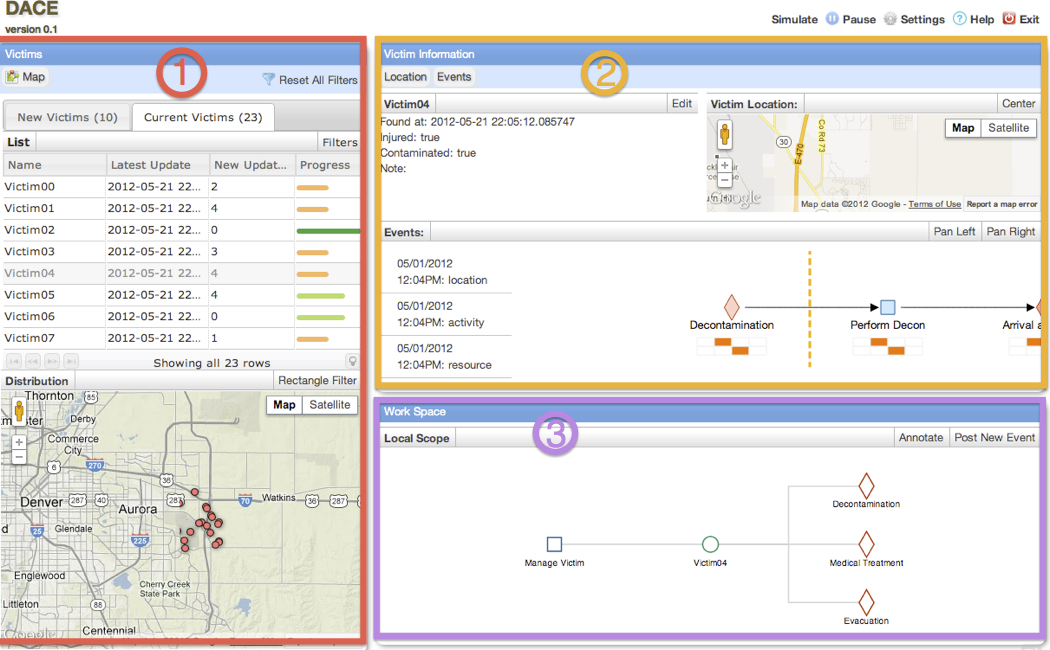
\includegraphics[width=5.5in]{main_interface.jpg} 
	\caption{The main interface of the EDAP client}
	\label{fig:main_interface}
\end{figure}


\begin{enumerate}
	\item The \emph{event view} provides a list of current events notified to the victim manager. The victim manager can click on each event to activate the event propagation tree to backtrack the event development.
	\item The \emph{activity view} shows the goals, activities, resources assigned to the current victim, which forms the local scope of the victim manager, where he/she can interpret the event and project state changes based on established understanding of the situation.
	\item The \emph{context view} consists of interactive data visualization tools to explore the contextual information. For the victim manager, the interface allows him/her to monitor the status of every victim that has been reported. A dynamic query interface is used for filtering the victims based on attributes, time, and geographical locations.
\end{enumerate}

\fxwarning{use the scenario to run through the whole process to demonstrate the functionalities: from notification, to event view, to activity view, to the generate new events, to manage subscription, to manage visibility. }
% section implementation_of_edap_client (end)
% chapter system_implementation (end)




 


%!TEX root = ../BoYu-Dissertation.tex
\graphicspath{{Figures/}}

\chapter{Our Approach: Mediating Awareness Propagation} % (fold)
\label{cha:mediate_awareness_propagation}

Activity representation as an approach to support awareness transactions between actors:

scenario-based design

a. the ability to find who should be awareness of certain events by making each other's local scopes visible

b. the ability to interpret events within the activity context

% chapter mediate_awareness_propagation (end)




 


%!TEX root = ../BoYu-Dissertation.tex
\graphicspath{{Figures/}}

\chapter{Conclusion} % (fold)
\label{cha:conclusion}
\section{Research Contributions} % (fold)
\label{sec:contributions}
Focusing on the design of a computational system to support awareness in collaborative activities with high level of complexity, this research fits into the design-science paradigm in information science \cite{Hevner2004}. As argued by Hevner et al \cite{Hevner2004}, effective design-science research must provide clear contributions in at least one of the following areas: (1) the development of constructs or models that extend and improve the understanding of the design problem (i.e. foundations), (2) the development of methods or tools that enable solutions to the design problem (i.e. design artifacts), (3) and the development or creative use of evaluation methods or new evaluation metrics (i.e. methodologies). In this study, we claim contributions in the first two areas. 

\paragraph*{A conceptual framework of awareness in complex collaborations} % (fold)
\label{par:a_conceptual_framework_of_awareness_in_complex_collaborations}
The first contribution of this research is the integrated conceptual framework for understand the awareness phenomena in complex collaborations. Our conceptual framework is built on top of existing theories and models for understanding the awareness phenomena in the literature, and in turn contribute to existing knowledge foundations in two aspects:

\begin{enumerate}
	\item We adopt several interrelated constructs, i.e. activity, local scope, and dependency, to understand the \emph{product} of awareness phenomena, i.e. what part of the world the collaborators should be aware of. These constructs together enrich the existing understanding of the awareness phenomena in collaborative environment. Beyond the knowledge sharing perspective, we emphasize the distributed nature of the awareness phenomena. Because of the differences in local scopes, each team member's awareness is partial, but at the same time is compatible for the team to perform collaborative activities successfully.
	\item We build on top of these constructs to understand the awareness \emph{process} in collaborative environments. Our framework is able to account for how the awareness is distributed across multiple team members. Comparing with existing models, our framework provides a better explanation of how the compatibility of different collaborators' awareness is achieved through the integration of individual cognitive processes and social processes.
\end{enumerate}

Beyond the theoretical contribution, this conceptual framework has also shown its value in guiding the design of awareness supporting tools in our study:

\begin{enumerate}
	\item First, it helps us to understand the design space of awareness support and identify key design issues to support awareness. By conceptualizing the awareness phenomena in distributed, complex collaboration as continuous developed through a variety of cognitive and social processes, the design issues for awareness support can be organized at both the individual level and the team level. The former focuses on supporting the cognitive processes of individual team members to develop their own awareness, while the latter provides support for the social processes in which team members interact with each other to achieve compatible awareness.
	\item Second, the conceptual framework also guides our design of the awareness promotion approach. On one hand, the knowledge representation of our approach is designed to comply with the the three constructs in the conceptual framework. As these constructs describe the configuration of the field of work that regulates how the awareness is distributed across team members, they provide the necessary knowledge for the system to reason about human actors' needs and promote awareness. Furthermore, one of the design principles of our awareness promotion is to consider the awareness support from a collective perspective and provide integrated support for the whole awareness development cycle, which is motivated by the understanding of the awareness process in the conceptual framework.
\end{enumerate}
% paragraph a_conceptual_framework_of_awareness_in_complex_collaborations (end)

\paragraph*{The awareness promotion approach} % (fold)
\label{par:the_awareness_promotion_approach}
The second major contribution of this study is the awareness promotion approach. This approach is based on two major design principles: (1) it aims to design a knowledge-based system that maintains a collective knowledge representation of the field of work, and utilizes it to support the various awareness processes; (2) it emphasizes the division of work between the computational system and human actors, and provides adequate interaction techniques to allow the human actors to collaborate with the computer to develop awareness. Following these design principles, the awareness promotion approach is built on top of two major components: a computational representation of the field of work based on the SharedPlan theory, and an event-driven model of the awareness processes. Then the computer system’s behaviors to promote awareness are embedded in the interaction between these two components. On one hand is how the computer constructs and develops the knowledge representation of the field of work within the event-driven processes, and on the other hand is how the knowledge representation is used to promote these event-driven awareness processes.

The awareness promotion approach has several advantages to handle the scaled up complexity and dynamics in collaborative activities, and provides integrated awareness support. 

\begin{enumerate}
	\item First, it utilizes the computational knowledge representation to model the field of work and offloads some of the representation and reasoning efforts from the human to the computer. Hence, it can handle more complex situations than existing awareness models.
	\item Meanwhile, the knowledge representation is dynamically updated to reflect the current state of the field of work, which allows it to handle increased level of dynamics.
	\item The awareness promotion approach shows much more frequent interactions between the computer and the human users. Each awareness process involves both the computer’s reasoning and the human’s cognition, as well as the interaction to combine them together.
\end{enumerate}

% paragraph the_awareness_promotion_approach (end)
% section contributions (end)

\section{Comparison with Existing Studies} % (fold)
\label{sec:comparison_with_existing_studies}

% section comparison_with_existing_studies (end)

\section{Future Directions} % (fold)
\label{sec:future_directions}
Behavioral study to understand the conceptualization.

Formal evaluation of the system. 

Extension to asynchronous 

Extension to multi-tasking

% section future_work (end)
% chapter conclusion (end)




 


%!TEX root = ../BoYu-Dissertation.tex
\graphicspath{{Figures/}}

\chapter{Case Studies} % (fold)
\label{cha:case_studies}
% chapter case_studies (end)




 


%!TEX root = ../BoYu-Dissertation.tex
\graphicspath{{Figures/}}

\chapter{Conclusion and Future Work} % (fold)
\label{cha:conclusion}

% chapter conclusion (end)




 



%%%%%%%%%%%%%%%%%%%%%%%%%%%%%%%%%%%%%%%%%%%%%%%%%%%%%%%%%%%%%%%
% Appendices
%
% Because of a quirk in LaTeX (see p. 48 of The LaTeX
% Companion, 2e), you cannot use \include along with
% \addtocontents if you want things to appear the proper
% sequence. Since the PSU Grad School requires 
%%%%%%%%%%%%%%%%%%%%%%%%%%%%%%%%%%%%%%%%%%%%%%%%%%%%%%%%%%%%%%%
\appendix
% \Appendix{Events Description in the Emergency Response Scenario}
\label{app:event_description}
\section{Episode 1: Goal activation} % (fold)
\label{sec:episode_1_goal_activation}
\footnotesize
{
	\begin{longtable}{>{\raggedright}p{1.2in}>{\raggedright}p{1.2in}>{\raggedright}p{3in}}
\toprule 
\textbf{Actor} & \textbf{Type} & \textbf{Description}\tabularnewline
\midrule 
Fireman & Generate event (E1) & E1: A new victim has been found at a given location within the impacted
area\tabularnewline
\midrule 
\multirow{3}{1.2in}{Victim manager (VM)} & Consume event (E1) & Upon receiving E1, VM activate the goal that the victim needs to be
rescued, and decomposes the action to rescue the victim into sub-actions.\tabularnewline
\cmidrule{2-3} 
 & Perform action & In order to rescue the victim, VM first evaluates the status of the
victim. 

Because the radiation level of the victim exceeds the threshold, the
victim needs to be first decontaminated.

Because the victim is also physically injured, the victim needs to
be treated at a medical station after decontamination.

After the treatment, the victim needs to be evacuated to a shelter
for recovery.\tabularnewline
\cmidrule{2-3} 
 & Generate events (E2, E3, E4) & E2: A new goal to decontaminate the victim is activated

E3: A new goal to treat the victim is activated

E4: A new goal to evacuate the victim is activated\tabularnewline
\midrule 
\multirow{3}{1.2in}{Decontamination manager (DM)} & Consume event (E2) & Upon receiving E2, DM infers that the action to decontaminate is within
her responsibility and she is capable of performing it, so she is
committed to performing the action, decompose the action into sub-actions.\tabularnewline
\cmidrule{2-3} 
 & Perform action & To perform decontamination, DM first needs to assign a decontamination
station to the victim.

After the assignment of station (DS1) to the victim, the DM activates
the goal to transport the victim to the station. \tabularnewline
\cmidrule{2-3} 
 & Generate event (E5, E6) & E5: The station (DS1) has been assigned to the decontamination action
on victim.

E6: A new goal to transport the victim to the assigned decontamination
station is activated\tabularnewline
\midrule 
Medical manager (MM) & Consume event (E3) & Upon receiving E3, MM infers that the action to treat the victim is
within her responsibility. However, because the action depends on
the action to decontaminate the victim to be completed first, she
has to wait for now.\tabularnewline
\midrule 
\multirow{4}{1.2in}{Transportation manager (TM)} & Consume event (E4) & Upon receiving E4, TM infers that the action to evacuate the victim
is within her responsibility.

However, because the action depends on the action to treat the victim
to be completed first, she has to wait for that first.\tabularnewline
\cmidrule{2-3} 
 & Consume event (E6) & Upon receiving E5, TM infers that the action to transport the victim
to the station is within her responsibility and she is capable of
performing it, so she is committed to performing the action, and further
decompose the action.\tabularnewline
\cmidrule{2-3} 
 & Perform action & TM first needs to assign a driver (DR1) with a rescue vehicle to the
action.

Because the actual transportation action is out of the DM's responsibility,
she is waiting for the driver to perform it.\tabularnewline
\cmidrule{2-3} 
 & Generate event (E7) & E7: The driver (DR1) has been assigned to the action to transport
the victim \tabularnewline
\midrule 
Driver (DR1) & Consume event (E7) & Upon receiving E6, DR1 infers that the action to transport the victim
to the station is within her responsibility and she is capable of
performing it, so she starts to perform the action.\tabularnewline
\bottomrule
\caption{Episode 1 in the emergency response scenario}
\label{tab:episode_1_appendix}
\end{longtable}
}

% section episode_1_goal_activation (end)

\section{Episode 2: Plan development} % (fold)
\label{sec:episode_2_plan_development}
\footnotesize
{
	\begin{longtable}{>{\raggedright}p{1.2in}>{\raggedright}p{1.2in}>{\raggedright}p{3in}}
\toprule 
\textbf{Actor} & \textbf{Type} & \textbf{Description}\tabularnewline
\midrule 
Operator at the decontamination station & Generate event (E1) & E1: The quantity of available rinse tanks in the station (DS1) is
running low.\tabularnewline
\midrule 
\multirow{3}{1.2in}{Decontamination manager (DM)} & Consume event (E1) & Upon receiving E1, DM infers that the station (DS1) cannot work properly
due to this resource shortage. In order to ensure the victim is successfully
decontaminated, a new action to resolve the resource shortage is added
to the current plan to rescue the victim. \tabularnewline
\cmidrule{2-3} 
 & Perform action & DM first needs to locate an inventory where the rinse tanks can be
supplied.

After identification of the inventory (INV1), the DM activates the
goal to deliver the resource from the inventory to the station. \tabularnewline
\cmidrule{2-3} 
 & Generate event (E2) & E2: A new goal to deliver the resource from (INV1) to the station
(DS1) is activated.\tabularnewline
\midrule 
\multirow{3}{1.2in}{Inventory manager (IM)} & Consume event (E2) & Upon receiving E2, IM starts a new action to deliver the resource.\tabularnewline
\cmidrule{2-3} 
 & Perform action & IM first needs to prepare the resource for delivery. Once the resource
is ready, she activates the goal to transport the resource to the
station (DS1)\tabularnewline
\cmidrule{2-3} 
 & Generate event (E3) & E3: A new goal to transport the resource to the station (DS1) is activated\tabularnewline
\midrule 
\multirow{3}{1.2in}{Transportation manager (TM)} & Consume event (E3) & Upon receiving E3, TM starts a new action to transport the resource.\tabularnewline
\cmidrule{2-3} 
 & Perform action & TM first needs to assign a driver (DR2) with a rescue vehicle to the
action.

Because the actual transportation action is out of the DM's responsibility,
she is waiting for the driver to perform it.\tabularnewline
\cmidrule{2-3} 
 & Generate event (E4) & E4: The driver (DR2) has been assigned to the action to transport
the victim \tabularnewline
\midrule 
Driver (DR2) & Consume event (E4) & Upon receiving E4, DR2 infers that the action to transport the victim
to the station is within her responsibility and she is capable of
performing it, so she starts to perform the action.\tabularnewline
\bottomrule
\caption{Episode 2 in the emergency response scenario}
\label{tab:episode_2_appendix}
\end{longtable}
}
% section episode_2_plan_development (end)

\section{Episode 3: Role transfer} % (fold)
\label{sec:episode_3_responsibility_transfer}
\footnotesize
{
\begin{longtable}{>{\raggedright}p{1.2in}>{\raggedright}p{1.2in}>{\raggedright}p{3in}}
\toprule 
\textbf{Actor} & \textbf{Type} & \textbf{Description}\tabularnewline
\midrule 
Driver (DR1) & Generate event (E1) & E1: The rescue vehicle with the driver (DR1) encounters a mechanical
breakdown.\tabularnewline
\midrule 
\multirow{3}{1.2in}{Transportation manager (TM)} & Consume event (E1) & Upon receiving E1, TM infers that because of the vehicle breakdown,
the DR1's action to transport the victim cannot be achieved.\tabularnewline
\cmidrule{2-3} 
 & Perform action & To solve the problem, TM attempts to assign another driver to the
action.

However, because all the drivers are currently in duty, the TM cannot
find a driver to perform the action until a later time.\tabularnewline
\cmidrule{2-3} 
 & Generate event (E2) & E2: The action to transport the victim has to be delayed because of
the unavailability of drivers.\tabularnewline
\midrule 
\multirow{2}{1.2in}{Decontamination manager (DM)} & Consume event (E2) & Upon receiving E2, DM infers that because of the delay to transport
the victim, the action to decontaminate the victim is also delayed.\tabularnewline
\cmidrule{2-3} 
 & Generate event (E3) & E3: The action to decontaminate the victim will be delayed because
of the delay of the transportation task.\tabularnewline
\midrule 
\multirow{2}{1.2in}{Victim manager (VM)} & Consume event (E3) & Upon receiving E3, VM infers that because of the delay to transport
the victim, the action to rescue the victim is delayed.\tabularnewline
\cmidrule{2-3} 
 & Generate event (E4) & E4: The action to rescue the victim is delayed because of the delay
of the transportation task.\tabularnewline
\midrule 
\multirow{2}{1.2in}{Fireman} & Consume event (E4) & Upon receiving E4, the fireman infers that although delivery of the
victim is not in the scope of her responsibility, however she can
help the rescue action by sending the victim to the decontamination
station (DS1). \tabularnewline
\cmidrule{2-3} 
 & Generate event (E5) & E5: The fireman activates the goal to send the victim to the decontamination
station (DS1). \tabularnewline
\midrule 
Transportation manager (TM) & Consume event (E5) & Upon receiving E5, TM infers that because of the new action of the
fireman, the responsibility of transporting the victim is now transferred
from her to the fireman.\tabularnewline
\bottomrule
\caption{Episode 3 in the emergency response scenario}
\label{tab:episode_3_appendix}
\end{longtable}
}
% section episode_3_responsibility_transfer (end)

\section{Episode 4: Opportunistic re-planning} % (fold)
\label{sec:episode_4_opportunistic_re_planning}
\footnotesize
{
	\begin{longtable}{>{\raggedright}p{1.2in}>{\raggedright}p{1.2in}>{\raggedright}p{3in}}
\toprule 
\textbf{Actor} & \textbf{Type} & \textbf{Description}\tabularnewline
\midrule 
Fireman & Generate event (E1) & E1: The physical injury of the victim becomes severe and prevents
the fireman from moving the victim into the vehicle.\tabularnewline
\midrule 
\multirow{2}{1.2in}{Victim manager (VM)} & Consume event (E1) & Upon receiving E1, VM evaluates the situation of the victim and decides
that because of the serious injury, the original plan to rescue the
victim is no longer appropriate. A new plan needs to be adopted: a
special team needs to be dispatched to the victim's location to decontaminate
and treat the victim on spot, and then the victim is directly sent
to the hospital for further treatment.\tabularnewline
\cmidrule{2-3} 
 & Generate events (E2, E3, E4, E5, E6) & E2: The current goal to decontaminate the victim is deactivated

E3: The current goal to treat the victim is deactivated

E4: The current goal to evacuate the victim is deactivated

E5: A new goal to dispatch a special team to the victim is activated

E6: A new goal to send the victim to the hospital is activated\tabularnewline
\midrule 
\multirow{4}{1.2in}{Decontamination manager (DM)} & Consume event (E2) & Upon receiving E2, DM removes the action to decontaminate the victim
from her current responsibility.\tabularnewline
\cmidrule{2-3} 
 & Consume event (E5) & Upon receiving E5, DM infers that in order to perform the action to
dispatch a special team to the victim, a decontamination operator
needs to be assigned to the team sent to the victim. \tabularnewline
\cmidrule{2-3} 
 & Perform action & By reviewing the available operators, DM decides on the operator that
will be sent to the victim\tabularnewline
\cmidrule{2-3} 
 & Generate event (E7) & The decontamination operator has been assigned to the special team
to the victim.\tabularnewline
\midrule 
\multirow{4}{1.2in}{Medical manager (MM)} & Consume event (E3) & Upon receiving E3, MM removes the action to treat the victim from
her current responsibility.\tabularnewline
\cmidrule{2-3} 
 & Consume event (E5) & Upon receiving E5, DM infers that in order to perform the action to
dispatch a special team to the victim, a paramedic needs to be assigned
to the team sent to the victim. \tabularnewline
\cmidrule{2-3} 
 & Perform action & By reviewing the available actors, DM decides on the paramedic that
will be sent to the victim\tabularnewline
\cmidrule{2-3} 
 & Generate event (E8) & The paramedic has been assigned to the special team to the victim.\tabularnewline
\midrule 
\multirow{5}{1.2in}{Transportation Manager} & Consume event (E4) & Upon receiving E4, TM removes the action to evacuate the victim from
her current responsibility.\tabularnewline
\cmidrule{2-3} 
 & Consume event (E5) & Upon receiving E5, TM infers that in order to perform the action to
dispatch a special team to the victim,  the action to transport the
team to the victim needs to be activated. \tabularnewline
\cmidrule{2-3} 
 & Perform action & TM first needs to assign a driver with a rescue vehicle to the action.
Because the deactivation of the original decontamination action, the
driver (DR2) who was assigned for delivering the equipment is now
available for this action.\tabularnewline
\cmidrule{2-3} 
 & Generate event (E9) & E9: The driver (DR2) has been assigned to the action to transport
the special team to the victim \tabularnewline
\cmidrule{2-3} 
 & Consume event (E6) & Upon receiving E6, TM infers that the action to send the victim to
hospital is within her responsibility.

However, because the action depends on other actions to be completed
first, she has to wait for those first.\tabularnewline
\midrule 
Driver (DR2) & Consume event (E9) & Upon receiving E9, DR2 starts to perform the action to transport the
special team to the victim.\tabularnewline
\bottomrule
	\caption{Episode 4 in the emergency response scenario}
	\label{tab:episode_4_appendix}
\end{longtable}
}

% section episode_4_opportunistic_re_planning (end)
% \include{Appendix-B/Appendix-B}
%%%%%%%%%%%%%%%%%%%%%%%%%%%%%%%%%%%%%%%%%%%%%%%%%%%%%%%%%%%%%%%
% ESM students need to include a Nontechnical Abstract as the %
% last appendix.                                              %
%%%%%%%%%%%%%%%%%%%%%%%%%%%%%%%%%%%%%%%%%%%%%%%%%%%%%%%%%%%%%%%
% This \include command should point to the file containing
% that abstract.
%\include{nontechnical-abstract}
%%%%%%%%%%%%%%%%%%%%%%%%%%%%%%%%%%%%%%%%%%%
} % End of the \allowdisplaybreak command %
%%%%%%%%%%%%%%%%%%%%%%%%%%%%%%%%%%%%%%%%%%%

%%%%%%%%%%%%%%%%
% BIBLIOGRAPHY %
%%%%%%%%%%%%%%%%
% You can use BibTeX or other bibliography facility for your
% bibliography. LaTeX's standard stuff is shown below. If you
% bibtex, then this section should look something like:
   \begin{singlespace}
   %\bibliographystyle{FG-bibstyle}
   \bibliographystyle{amsplain}
   \addcontentsline{toc}{chapter}{Bibliography}
   \bibliography{library}
   %\nocite{*}
   \end{singlespace}

%\begin{singlespace}
%\begin{thebibliography}{99}
%\addcontentsline{toc}{chapter}{Bibliography}
%\frenchspacing

%\bibitem{Wisdom87} J. Wisdom, ``Rotational Dynamics of Irregularly Shaped Natural Satellites,'' \emph{The Astronomical Journal}, Vol.~94, No.~5, 1987  pp. 1350--1360.

%\bibitem{G&H83} J. Guckenheimer and P. Holmes, \emph{Nonlinear Oscillations, Dynamical Systems, and Bifurcations of Vector Fields}, Springer-Verlag, New York, 1983.

%\end{thebibliography}
%\end{singlespace}

%%%%%%%%%%%%%%%%
% Todo list %
%%%%%%%%%%%%%%%%
\todos

\backmatter

% Vita
%\vita{SupplementaryMaterial/Vita}

\end{document}

